\chapter{Build Instructions}%
\label{c:build}%
This chapter explains step by step the individual steps that are necessary to build an Open3DScanner from the individual components.%

The individual work steps are grouped together to summarize similar tasks.%

\section{Printing the Parts}%
First, the required parts must be printed for assembly. As mentioned before, I recommend using ABS filament as it's the only type of filament I've tested for the Open3DScanner, but I assume that other materials like PLA and PETG will work as well.%

So just use PLA if you can't print ABS with your 3D printer, for example because you don't have a closed print area or a heated print bed.%

The parts of the Open3DScanner were designed so that they all fit into the print volume of an \hrefIdx{https://www.prusa3d.com/original-prusa-i3-mk3/}{Original Prusa i3 MK3} (at least individually). This ensures that most 3D printers are able to print the parts for the Open3DScanner.%

The tolerance for the connections between the parts, as well as for screw holes etc. is \SI{0.35}{\milli\meter} for all parts at all points\marginTips[Test print]{It may be helpful to print a part as a sample and check that the tolerances used are appropriate for the printer being used.}.%

With the exception of the Rotor-Stand and Passive-Stand files, all files can be printed without support. For the two mentioned objects it is necessary to print support in the areas where the bearings are inserted. Apart from the removal of the support, no post-processing of the parts is necessary.%

\infoInfo{Note}{The assignment of the components to colours is arbitrary and corresponds to my personal taste. Of course it is possible to deviate from this "recommendation", it should only be pointed out that this allocation was used for the calculation of the necessary quantities of filament.}%

The following table lists which part has to be printed how often.%

\begin{table}[ht!]%
	\sideCaptionOf{table}{Quantity and color of 3D printed parts}%
	\rowcolors{2}{tableLineTwo}{tableLineOne}% specify rowcolors in tabularx style
	\begin{tabularx} {\linewidth} {>{\rowmac \hsize=\hsize}X>{\rowmac \hsize=\hsize}X>{\rowmac \hsize=\hsize}X<{\clearrow}}%
		\tabularxHeader%
		Part & Quantity & Color\\%
		Rotor-Arm  & 2 & Primary\\%
		Spotligt-Frame  & 1 --- 4 & Primary\\%
		Turntable-Arm  & 1 & Primary\\%
		Housing-Top  & 1 & Primary\\%
		Cable-Holder  & 5 & Primary\\%
		Backplate-Holder  & 2 & Primary\\%
		Turntable-Medium  & 1 & Secondary\\%
		Passive-Stand  & 1 & Secondary\\%
		Rotor-Stand  & 1 & Secondary\\%
		Spotligt-Stand  & 1 --- 4 & Secondary\\%
		Housing-Main  & 1 & Secondary\\%
		Housing-Plate  & 1 & Secondary\\%
		LCD-Holder  & 4 & Secondary\\%
		LED-Holder  & 1 & Secondary\\%
		Encoder-Holder  & 1 & Secondary\\%
		Micro-Fit-Holder-P1  & 4 & Secondary\\%
		Micro-Fit-Holder-P2  & 4 & Secondary\\%
		Food-Holder-Clamp  & 4 & Secondary\\%
		Rotor-Gear  & 1 & Accent\\%
		Rotor-Pinion  & 1 & Accent\\%
		Housing-Knob  & 1 & Accent\\%
	\end{tabularx}%
\end{table}%

% Primary: 477.30g
% Secondary: 810.67g
% Accent: 46.93g

The print settings for the objects are specified below. It is assumed that a \SI{0.4}{\milli\meter} nozzle is used. For other nozzles the values have to be adjusted accordingly.%

\begin{table}[ht!]%
	\sideCaptionOf{table}{Print settings for 3D printed parts with \SI[text-rm=\lightBoldFont]{0.4}{\milli\meter} nozzle}%
	\rowcolors{2}{tableLineTwo}{tableLineOne}% specify rowcolors in tabularx style
	\begin{tabularx} {\linewidth} {>{\rowmac \hsize=\hsize}X>{\rowmac \hsize=\hsize}X<{\clearrow}}%
		\tabularxHeader%
		Setting & Value\\%
		Layer height & \SI{0.2}{\milli\meter}\\%
		Perimeters & 4\\%
		Solid top layers & 5\\%
		Solid bottom layers & 5\\%
		Infill & \SI{40}{\percent}\\%
	\end{tabularx}%
\end{table}%

The amount of print settings listed in the table is kept as small as possible in order to describe only slicer independent settings.%

In particular, the use of a specific slicer is not necessary for successful printing. When selecting the remaining settings, it is only necessary to ensure that the printed objects are as stable as possible.%

The 3D models for the objects are all available in the orientation in which it is recommended to print them. The parts are aligned in such a way that the stability of the individual parts is improved under later loads (e.g. turntable arm) or that the quality of the printed details is improved in areas where this is important (e.g. spotlight frame).%

In case you stick to my color scheme and you build the maximum of four lights you will need a little bit over one \SI{800}{\gram} roll of filament of the secondary color. In total you need about \SI{500}{\gram} primary color filament, \SI{850}{\gram} secondary color filament, and \SI{80}{\gram} accent color filament.%

\section{Assembly the PCB}%
\label{sec:assPCB}%

This section describes how to assemble the PCB. This is not a step by step guide, but I pick up some special and important points and describe them.%

Such a step by step instruction for soldering the board is not included in this document. The only comparable one is a picture series, which documents all steps, which I have done during the assembly of the board. This picture series can be found in Appendix~\ref{cha:picSerPCB}.%

Instead, the board should be assembled in the way that is easiest for you. All components have an identifier, which can be found in the BOM and is printed on the PCB.%

\subsection{Preparing Pin Headers \& Sockets}%
Since both pin headers and pin sockets were purchased as 40 pin versions, it is necessary to cut the headers and sockets into suitable pieces before use.%

\marginElement{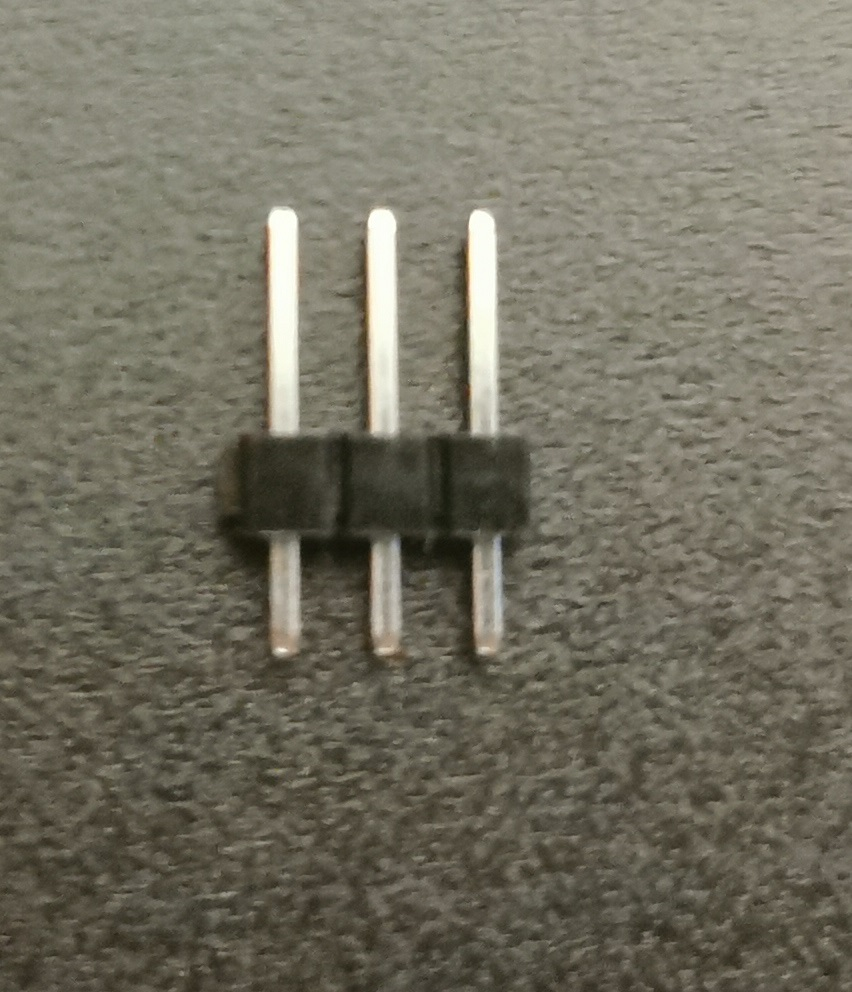
\includegraphics[width=\linewidth]{images/PinHeader.jpg}\captionof{figure}{The notches between the pins simplify separation}\label{fig:pinHeader}}%

With the pin headers, the process is very simple, since there is always a notch between the pins where the headers can be separated with a side cutter. Figure~\ref{fig:pinHeader} shows a three pin header with the clearly visible notches.%

With pin sockets this process is not as easy as with pin headers. Because of missing space there are no notches between the pins.%

For this reason it is necessary to first remove a pin with pliers, at which the strip should be separated. If a five pin socket is needed, the sixth pin is removed. Afterwards the socket is cut carefully with a side cutter at the now free place. This allows the sockets to be separated safely and reliably. The rough edges can be smoothed with the side cutter. The process is shown in figure~\ref{fig:pinSocket}.%

\begin{figure}[ht!]%
	\begin{centered}%
		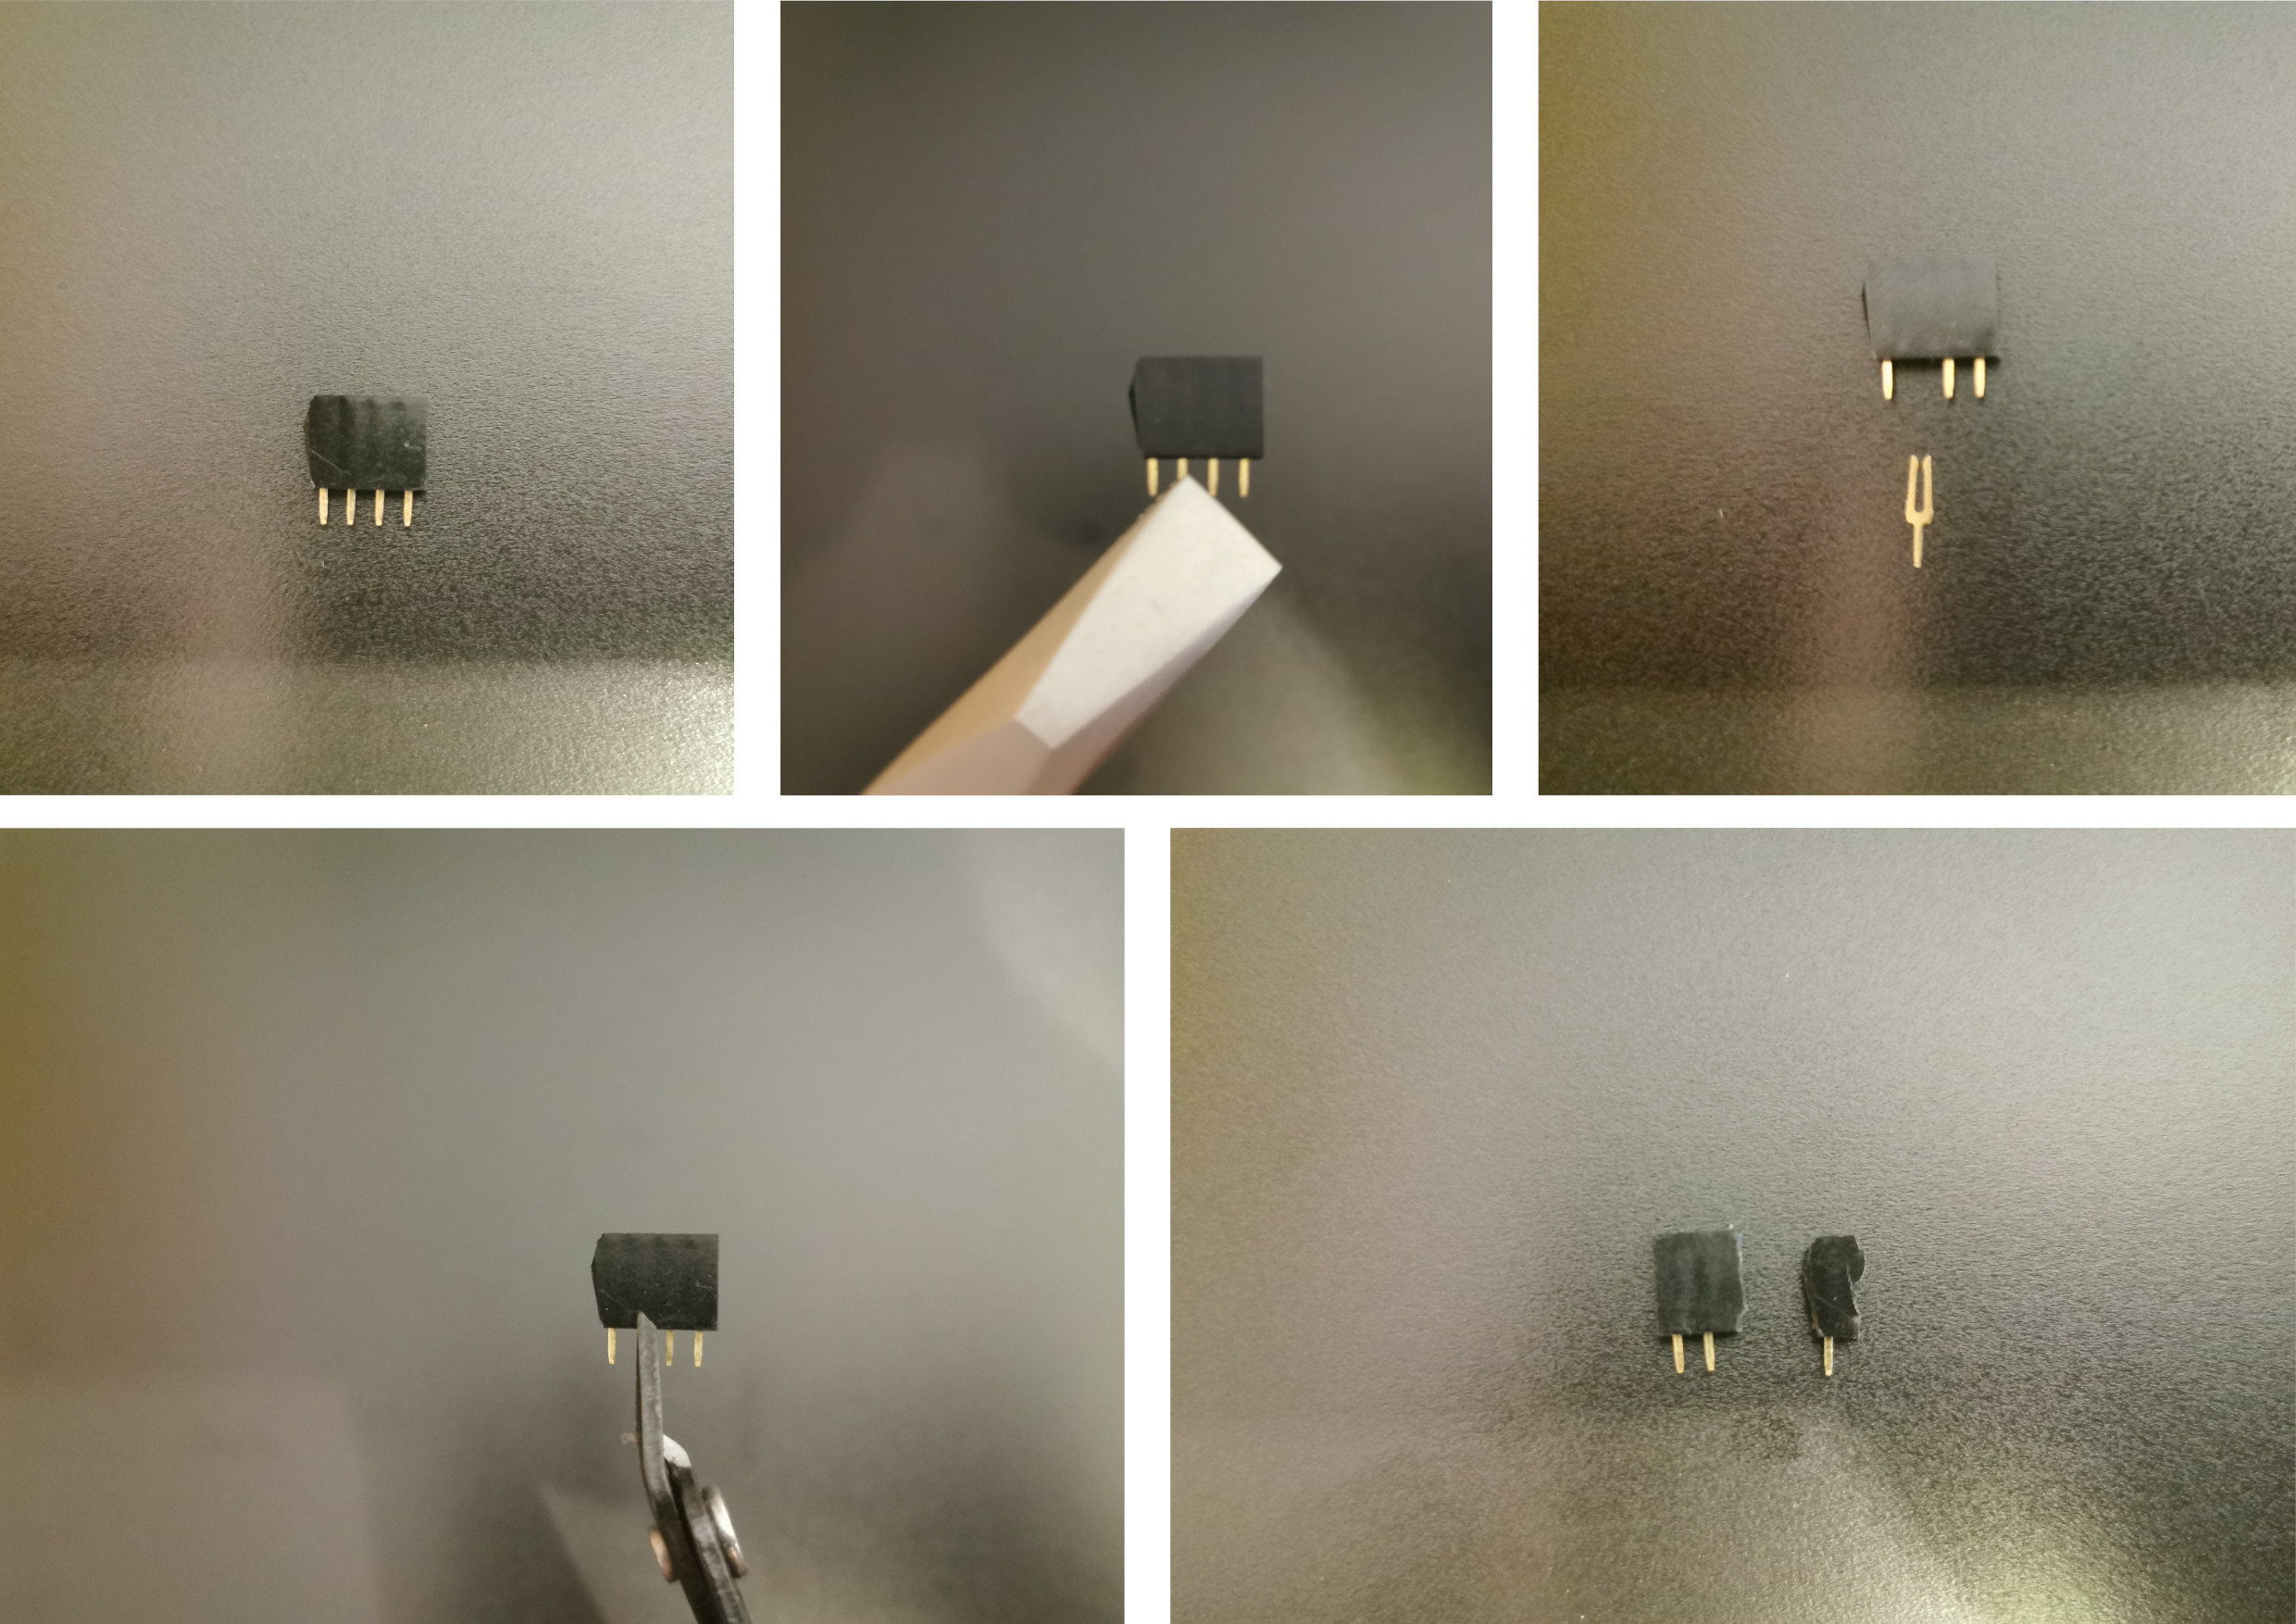
\includegraphics[width=\linewidth]{images/PinSocket.jpg}%
		\caption{How to separate pin sockets}%
		\label{fig:pinSocket}%
	\end{centered}%
\end{figure}%

\subsection{Assemble Pin Sockets}
The components which are mounted on pin sockets are the \hrefIdx{https://www.pololu.com/product/1182}{A4988 Stepper Drivers} and the \hrefIdx{https://www.espressif.com/en/products/hardware/esp32-devkitc/overview}{ESP32-DevKitC}.%

Both these components have two pin rows. It is therefore important that the pin sockets are mounted straight and parallel on the PCB so that the components can be inserted later.%

Without assistive tools, this is a pretty fiddly task. The simplest solution to this problem is to plug the pin sockets onto the corresponding components and solder them to the PCB. This ensures that the components fit exactly later.%

\subsection{TO-220 \& A4988 Cooling}%
The Open3DScanner does not use active cooling, but it is recommended to cool some parts passively.%

On the one hand the \hrefIdx{https://www.pololu.com/product/1182}{A4988 Stepper Drivers} should be equipped with a heat sink. If the stepper drivers get too warm, you may experience strange behavior (like missed steps). This is especially true if the stepper drivers are set to above \SI{1}{\ampere}.%

Furthermore, there are two \hrefIdx{https://www.centralsemi.com/PDFS/CASE/TO\_220\_PD.PDF}{TO-220} components on the board: the \hrefIdx{https://www.infineon.com/cms/en/product/power/mosfet/12v-300v-n-channel-power-mosfet/irlb8721/}{IRLB 8721} and the \hrefIdx{https://www.analog.com/en/products/lt1086.html}{LT1086CT-5}. The \hrefIdx{https://www.analog.com/en/products/lt1086.html}{LT1086CT-5} generates a lot of heat during operation, which can shorten the lifetime of the component considerably. For this reason I strongly recommend the use of thermal paste and a suitable heat sink.%

\marginElement{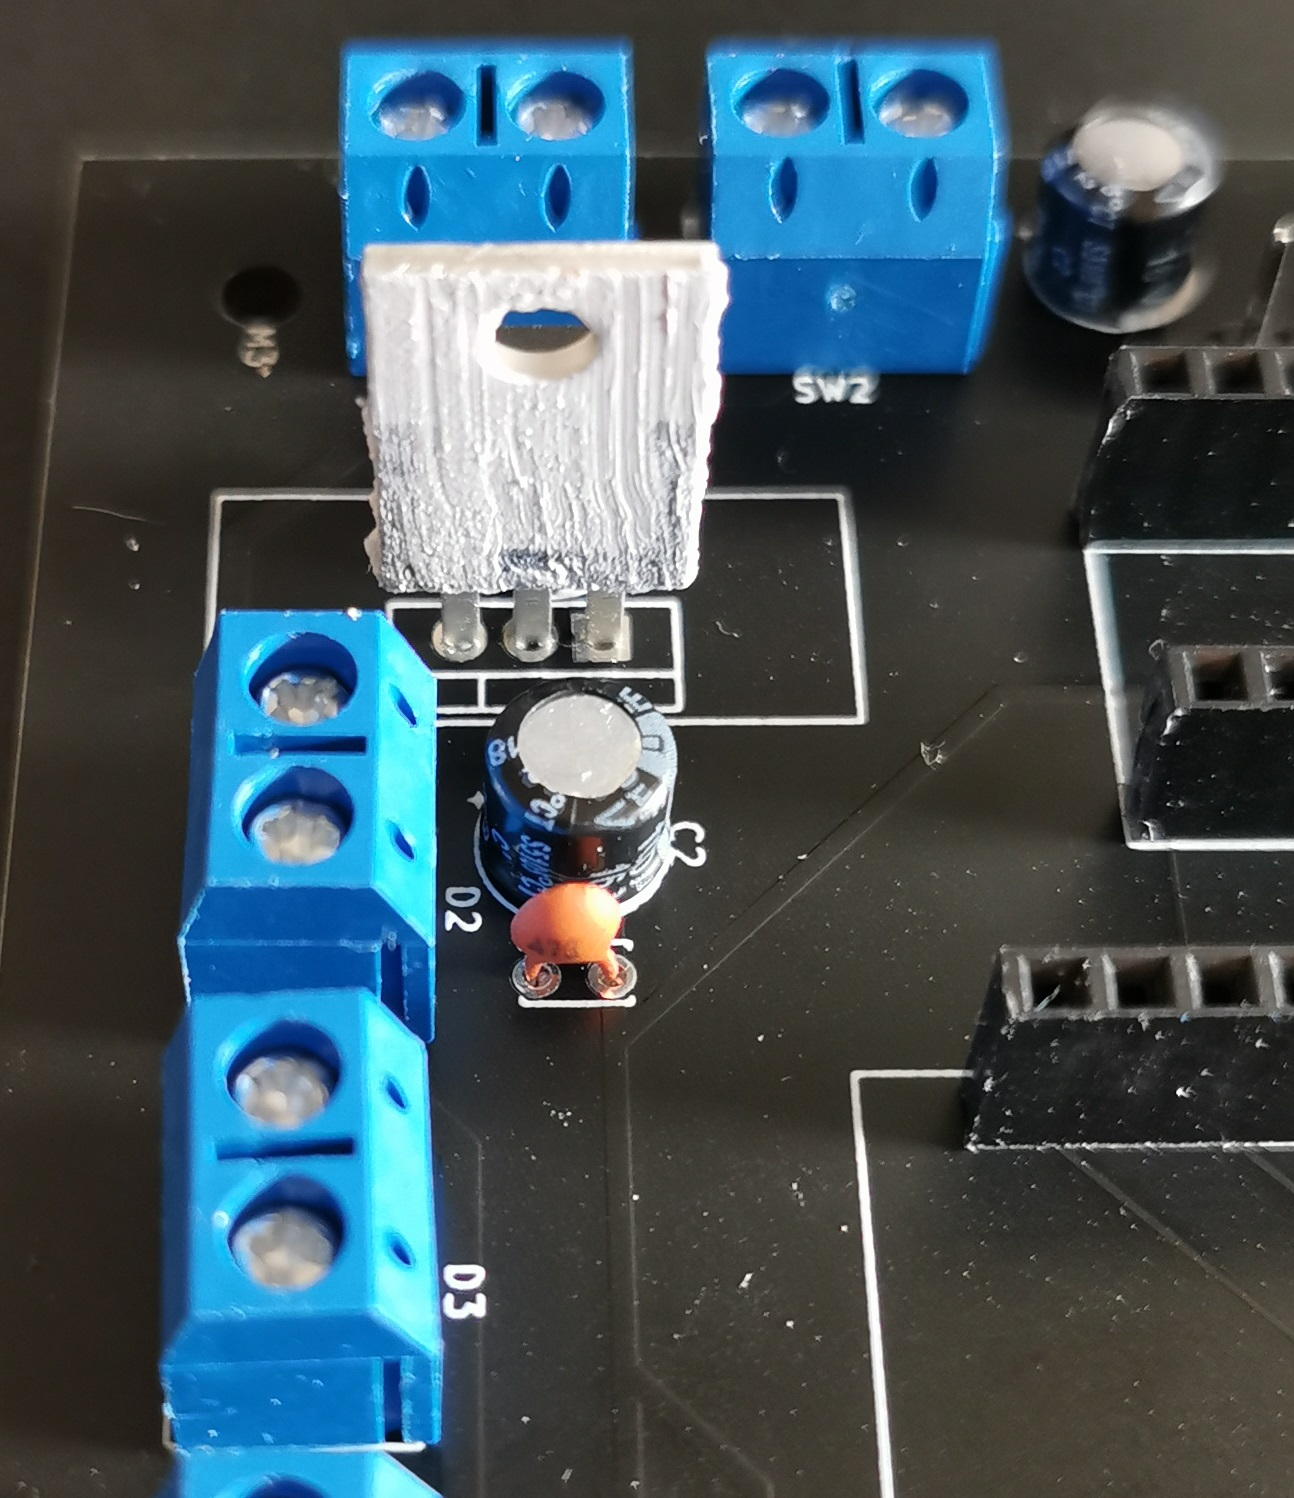
\includegraphics[width=\linewidth]{images/ThermalPaste.jpg}\captionof{figure}{Apply a thin layer of thermal paste\dots}}%
\marginElement{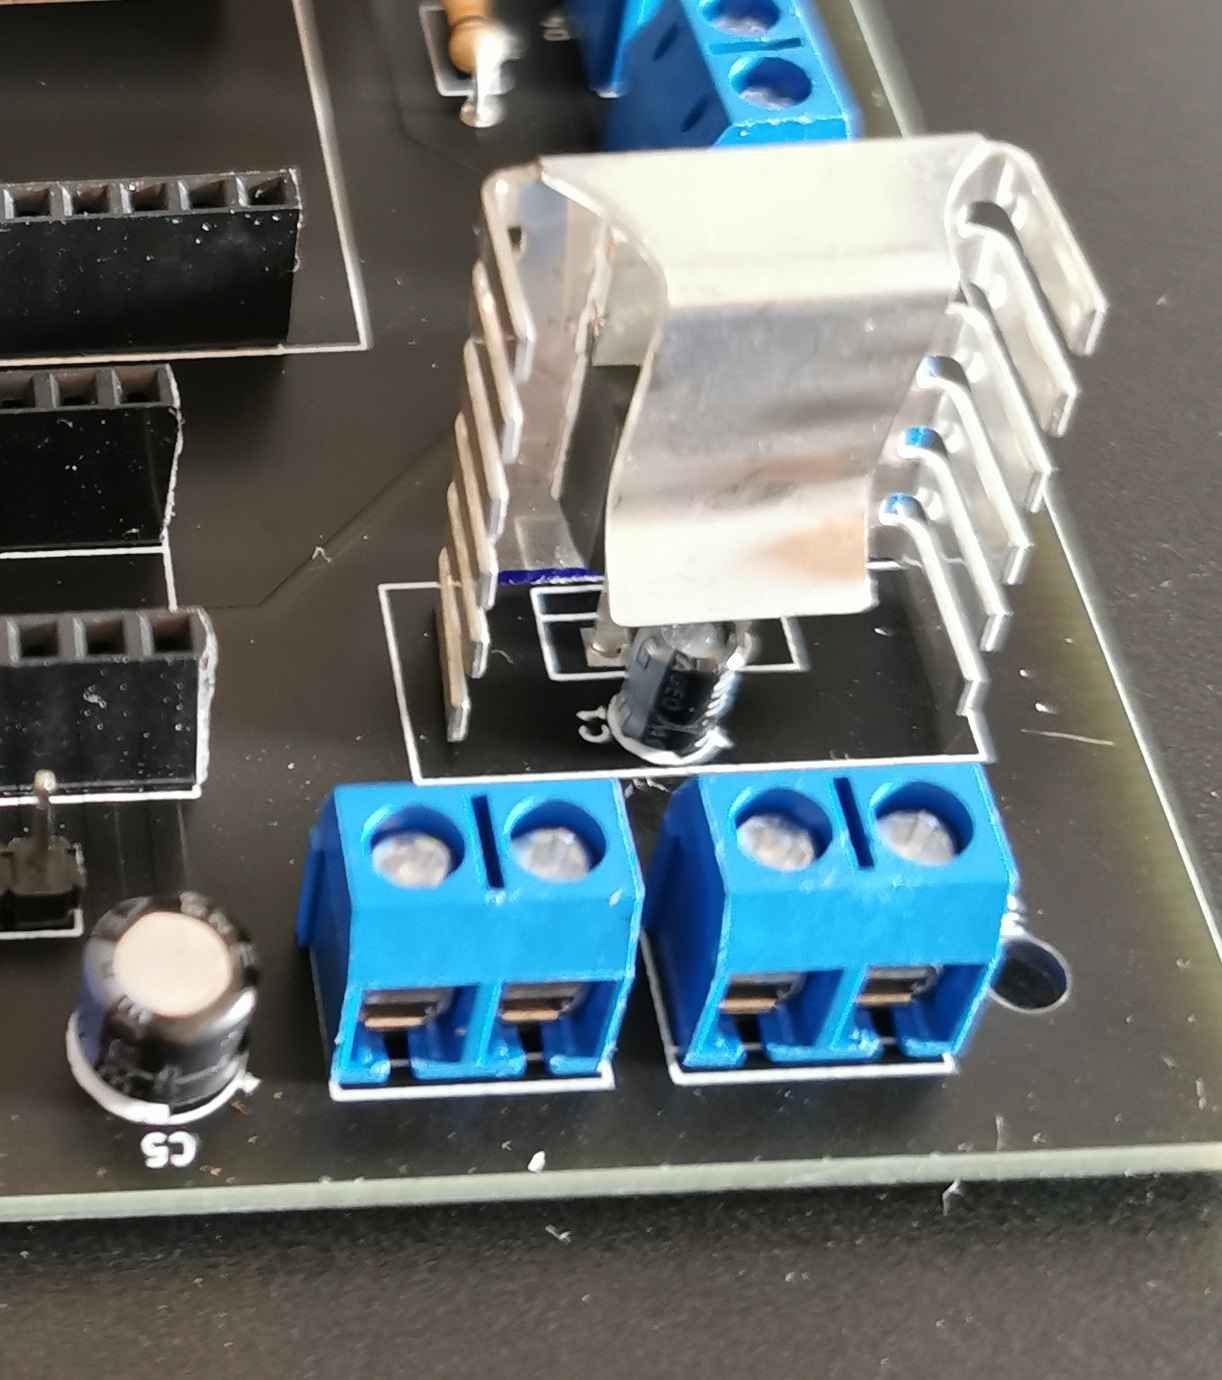
\includegraphics[width=\linewidth]{images/HeatSink.jpg}\captionof{figure}{\dots before installing the heat sink}}%

For the \hrefIdx{https://www.infineon.com/cms/en/product/power/mosfet/12v-300v-n-channel-power-mosfet/irlb8721/}{IRLB 8721} I didn't check to what extent it generates heat during operation, but according to the principle "better safe than sorry" I recommend the use of heat conducting paste and heat sink.%

Make sure that the heat sinks do not touch any other components or the circuit board. Especially with the \hrefIdx{https://www.analog.com/en/products/lt1086.html}{LT1086CT-5} it is a bit tight, because a high packing density is needed for an optimal function of the component.%

If you are using the TO-220 heat sinks I specified in the BOM, please note the following: Depending on how deep the pins are inserted into the PCB before soldering, it may be necessary to remove the bottom fin from the heat sink. Otherwise the heat sinks do not fit on the PCB, because they cannot put pressure on the component, which is necessary with the attachable heat sinks.%

\subsection{Prepare the LED Strip}%
The instructions in this section must be repeated for each light that will be connected to the Open3DScanner. While it is possible to operate the Open3DScanner with up to four lights simultaneously, I only use two.%

For the construction of the lights it is first necessary to prepare the LED strip. The LED strip is marked at regular intervals. At these markings it is possible to divide the strip.%

For the lights of the Open3DScanner \SI{15}{\centi\meter} long strips are needed. This corresponds to three segments of three LEDs. Figure~\ref{fig:ledStrip} shows such a \SI{15}{\centi\meter} piece of LED strip.%

\begin{figure}[ht!]%
	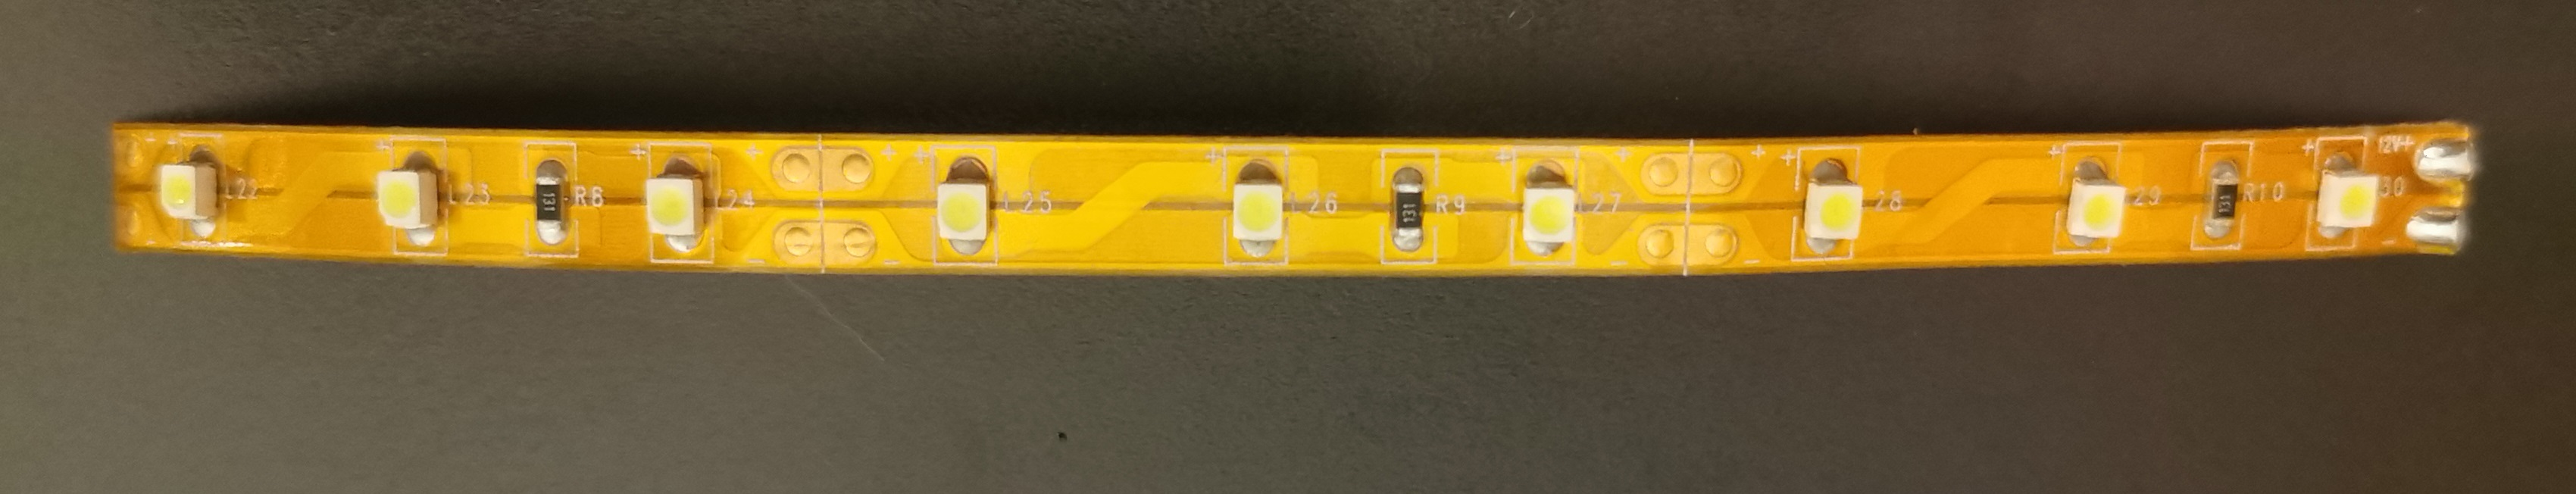
\includegraphics[width=\linewidth]{images/LedStrip.jpg}%
	\caption{One piece of LED strip as used in the Open3DScanner}%
	\label{fig:ledStrip}%
\end{figure}%

Each light of the Open3DScanner uses eight of these short strips and thus 72 LEDs.%

\begin{figure}[ht!]%
	\begin{centered}%
		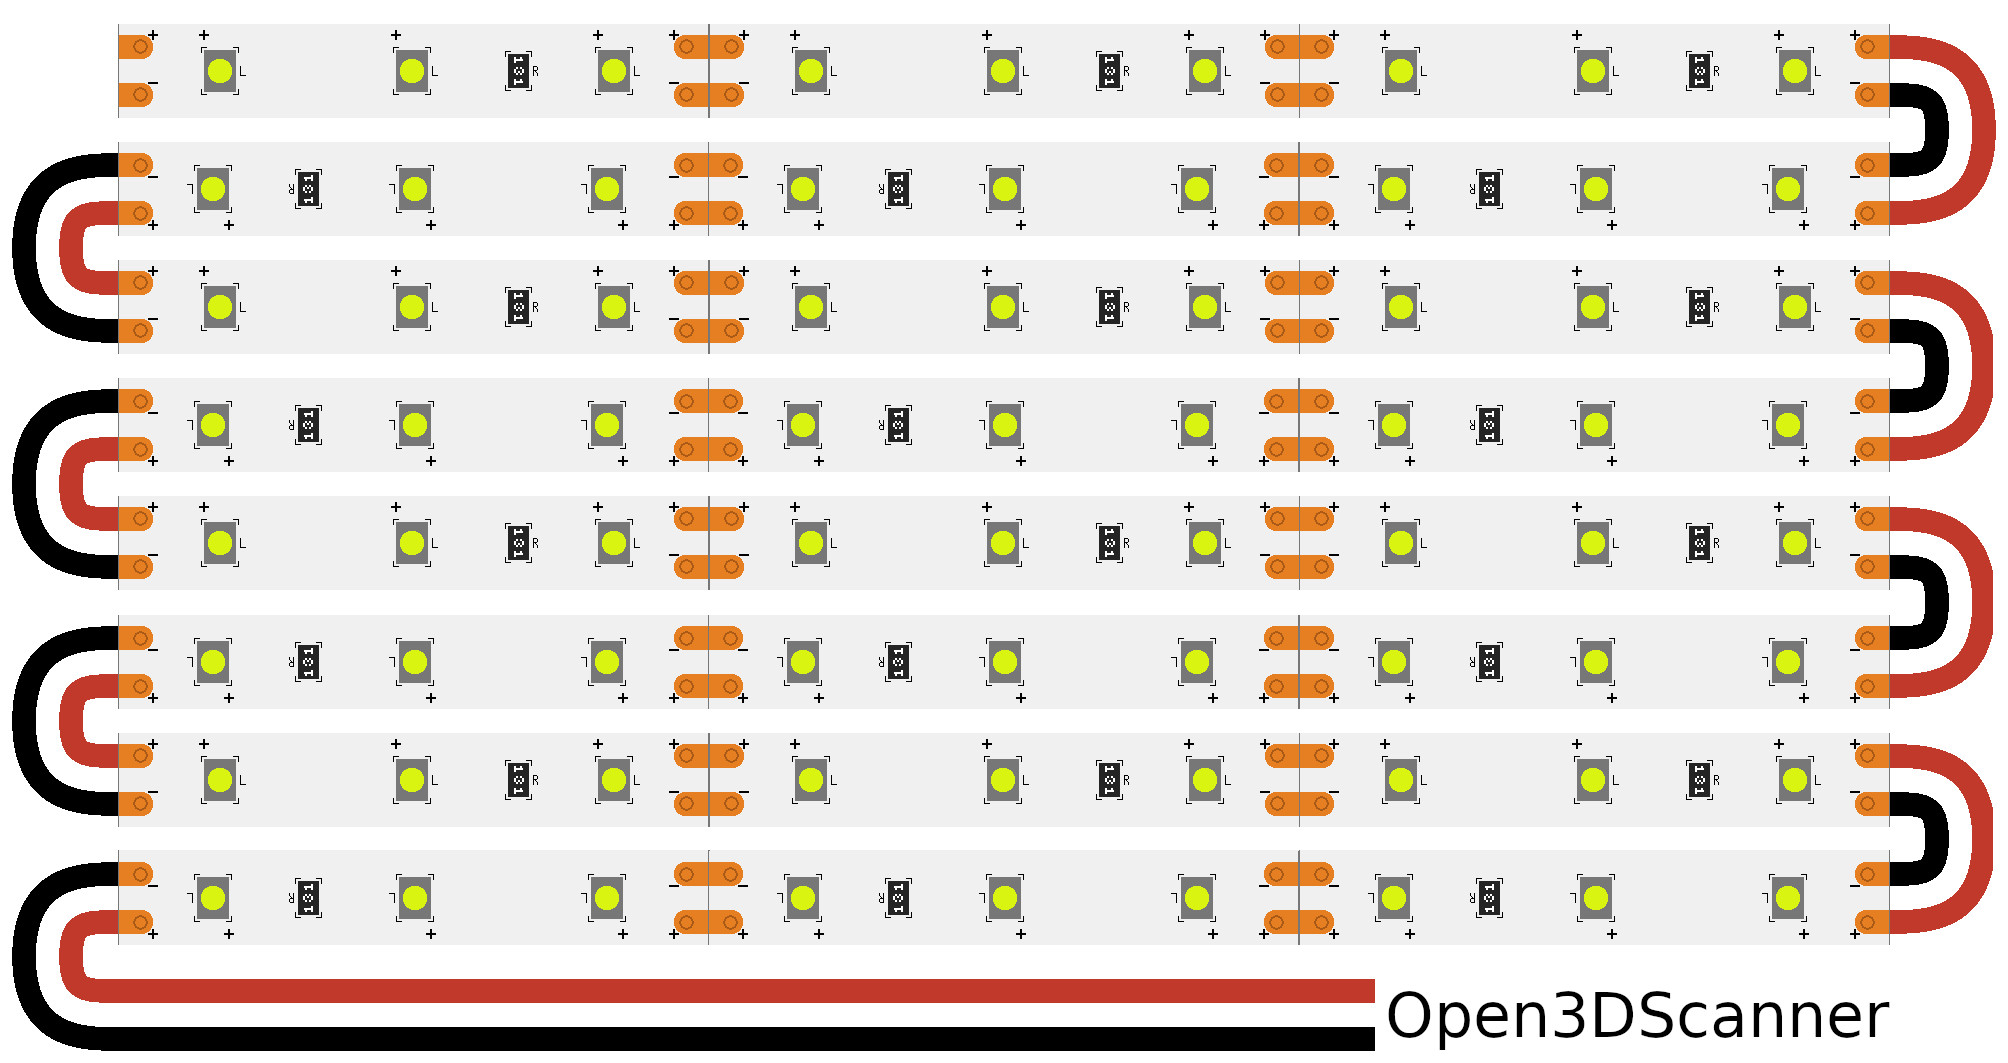
\includegraphics[width=\linewidth]{images/LedStripAssembly.jpg}%
		\caption{Schematic representation of the soldered LED strip for one light}%
		\label{fig:ledStripAssembly}%
	\end{centered}%
\end{figure}%

After dividing the LED Strip we need seven about \SI{7}{\centi\meter} long pieces of \SI{0.75}{\milli\meter\squared} cable with two wires each (for + and -). These are used to connect the segments of the LED strip to each other. We also need a approx. \SI{60}{\centi\meter} cable, which is used for the connection to the Open3DScanner. This cable can be shortened as soon as the lights are mounted and the cable is properly laid.%

Now the individual pieces of the LED strip are soldered together in series and the long cable is soldered to one end.%

It is important that no Molex connector is attached to the long cable at this point, otherwise we will not be able to lay the cable as intended. In general, it makes sense to attach the connector after the cable has been shortened to the correct length.%

A schematic representation of how the result of the soldering should look like can be found in figure~\ref{fig:ledStripAssembly}. When soldering, be sure to connect the right contacts.%

Now the soldered LED strip is glued to the Spotlight-Frame. One strip is glued in the middle of each of the recesses. Make sure that the long cable is at the lower end.%

\marginElement{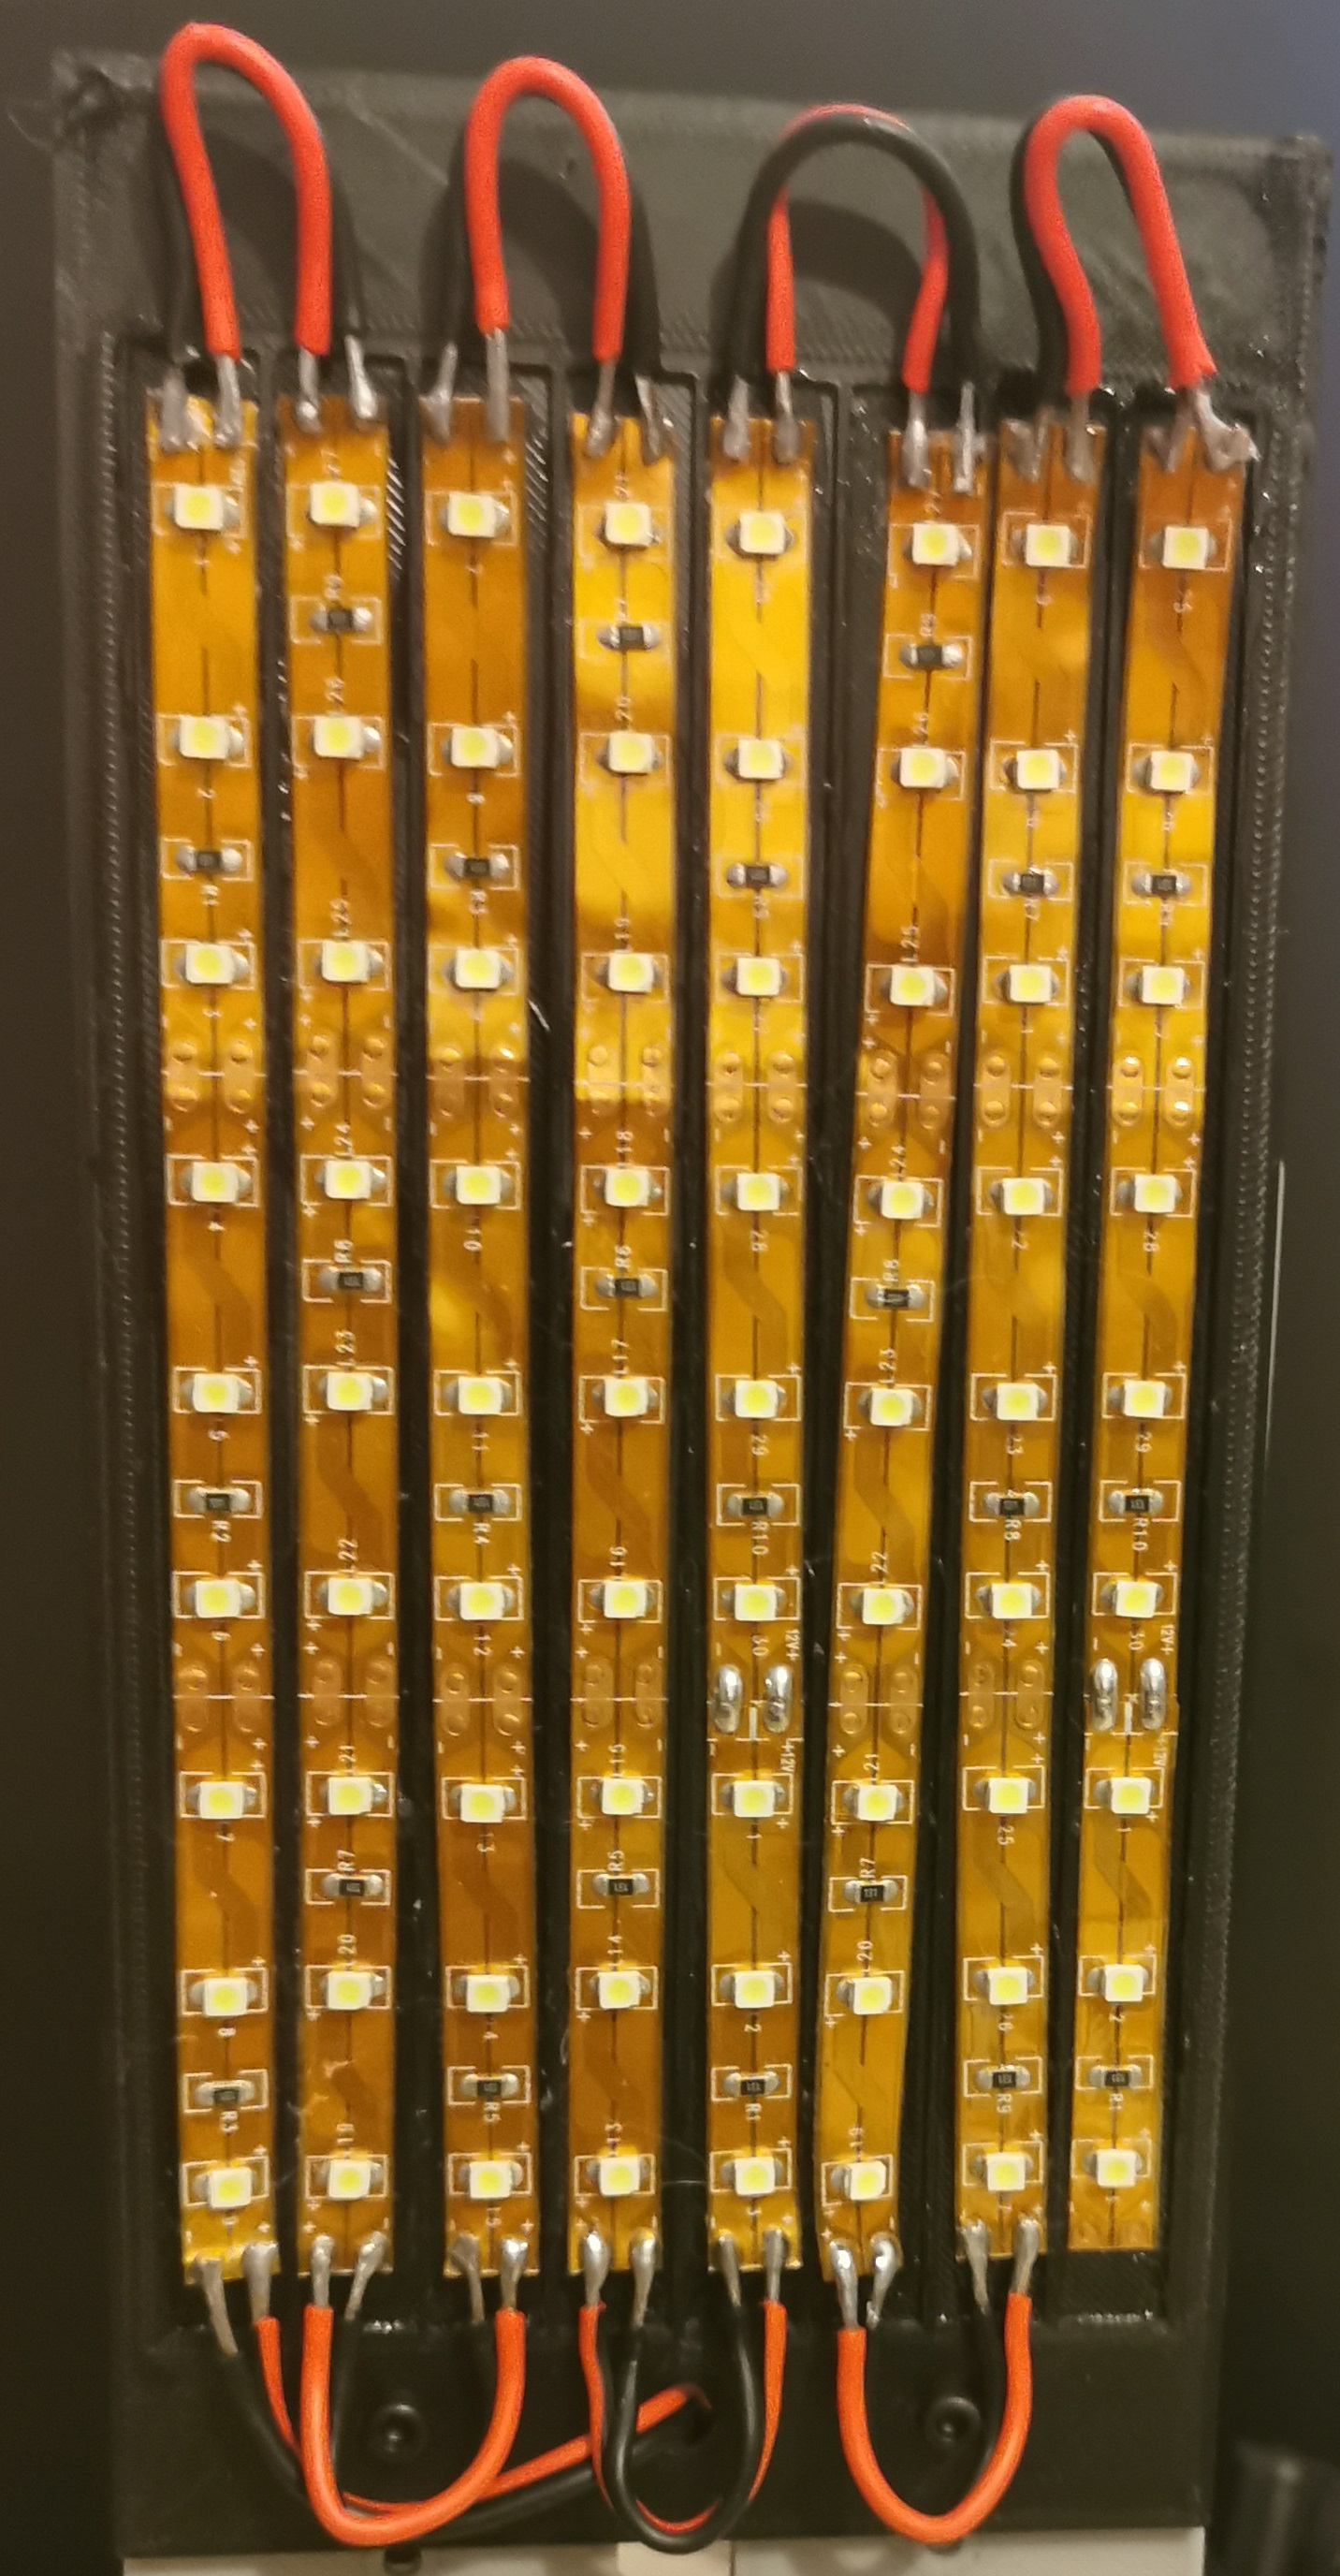
\includegraphics[width=\linewidth]{images/LedStripGlue.jpg}\captionof{figure}{Soldered LED strip glued into printed part}\label{fig:ledStripGlue}}%

The end of the long cable is led through the hole, which is in the lower area, in the middle of the part. Figure~\ref{fig:ledStripGlue} shows what the result should look like.%

The LED strip is glued in with the pre-assembled M3 adhesive tape. If this is not strong enough and the LED strips come loose again, you can simply spread some liquid glue on the printed part and then press the LED strip in again.

The LED strip is now ready for the assembly of the light which is described in section~\ref{sec:assembly}.

\subsection{Preparing the Cables}
In this section the cables used in the Open3DScanner are described in more detail. This is explicitly not a manual for crimping, there are very good sources for this\sideNote{There are many good instructions for crimping various connections on the Internet. For example, for crimping \hrefIdx{https://www.instructables.com/id/Dupont-Crimp-Tool-Tutorial/}{Dupont cables}, \hrefIdx{https://www.molex.com/molex/common/staticLoader.jsp?fileName=/tnotes/crimp.html\&progLink=Good+Crimps\&\&channel=...Micro-Fit\&channelId=0}{Molex Micro Fit}, and \hrefIdx{https://www.klauke.com/en/electrical/sectors-solutions/technical-reports/crimping-cable-lugs-correctly/}{cable lugs}. {\faYoutube} \hrefIdx{https://www.youtube.com/results?search\_query=crimping+tutorial}{YouTube} is a great source for tutorials, too.}.%

Instead, the following paragraphs describe the individual cables and their connections.%

A schematic diagram is given for each cable, which clearly shows how cables are aligned, if necessary.%

Power cables are shown in red (+) and black (GND), while all data cables are shown in blue. This colour coding is reused in later illustrations and thus simplifies orientation.%

The cable lengths specified do not include the length of the connectors which are used for each cable.%

\paragraph{LED Strip}\mbox{}\\%

\sideTabularx[LED strip cable characteristics]{%
	\rowcolors{2}{tableLineTwo}{tableLineOne}% specify rowcolors in tabularx style
	\begin{tabularx} {\marginparwidth} {>{\rowmac \hsize=\hsize}X>{\rowmac \hsize=\hsize}X<{\clearrow}}%
		\tabularxHeader%
		Characteristic & Value\\%
		Quantity & 4\\%
		Wire Gauge & \SI{0.75}{\milli\meter\squared}\\%
		Length & \SI{15}{\centi\meter}\\%
		End A Connector & Ferrule Crimp\\%
		End B Connector & Micro-Fit - 1x2-pin, male\\%
		End A connects & PCB contacts D2, D3, D4, D5\\%
		End B connects & Open3DScanner housing\\%
	\end{tabularx}%
}%

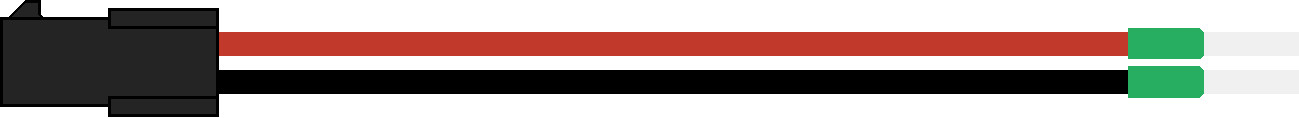
\includegraphics[width=\linewidth]{images/LedStripCable.jpg}%
{\captionof{figure}{Schematic representation of the LED strip cable}}% Take note of the surrounding {} to encapsulate special format settings

During assembly, the Molex connectors are clamped into the housing of the Open3DScanner so that they are directly accessible from the outside and the lights can be connected with a suitable Molex plug.%

Since ferrule crimps are necessary for the \SI{0.75}{\milli\meter\squared} cables, they may sit very tight in the screw terminals afterwards, which is no problem.%

Even if no or less than four lights will be connected to the Open3DScanner, it is necessary to prepare four of these cables so that there will be no gaps in the case later.%

The corresponding female connectors need to be added to the LED strips. This cable is not shown here. Just ensure that the polarity matches these cables.%

\clearpage%

\paragraph{Power Cables}\mbox{}\\%

\sideTabularx[Power connection cable characteristics]{%
	\rowcolors{2}{tableLineTwo}{tableLineOne}% specify rowcolors in tabularx style
	\begin{tabularx} {\marginparwidth} {>{\rowmac \hsize=\hsize}X>{\rowmac \hsize=\hsize}X<{\clearrow}}%
		\tabularxHeader%
		Characteristic & Value\\%
		Quantity & 2\\%
		Wire Gauge & \SI{0.75}{\milli\meter\squared}\\%
		Length & \SI{16/20}{\centi\meter} (Power Jack/Rocker Switch)\\%
		End A Connector & Ferrule Crimp\\%
		End B Connector & Cable Lug\\%
		End A connects & PCB contacts J1, SW2\\%
		End B connects & Rocker Switch \& Power Jack\\%
	\end{tabularx}%
}%

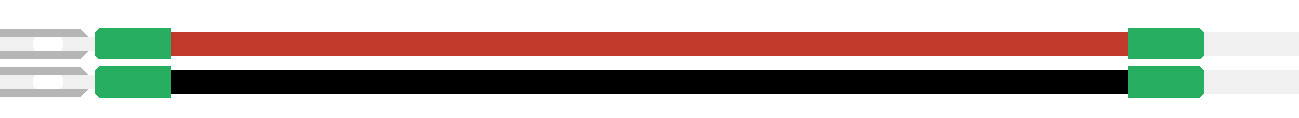
\includegraphics[width=\linewidth]{images/PowerCable.jpg}%
{\captionof{figure}{Schematic representation of the power connection cable}}% Take note of the surrounding {} to encapsulate special format settings

Two identical cables are used to connect the power source to the PCB and to connect the rocker switch, which allows the device to be switched on and off.%

Make sure that the correct cable lugs are used for both cables. These can be different for different versions of the parts and must be selected appropriately for the components.%

\paragraph{USB Cable}\mbox{}\\%

\sideTabularx[USB cable characteristics]{%
	\rowcolors{2}{tableLineTwo}{tableLineOne}% specify rowcolors in tabularx style
	\begin{tabularx} {\marginparwidth} {>{\rowmac \hsize=\hsize}X>{\rowmac \hsize=\hsize}X<{\clearrow}}%
		\tabularxHeader%
		Characteristic & Value\\%
		Quantity & 1\\%
		Wire Gauge & Undefined\\%
		Length & \SI{15}{\centi\meter}\\%
		End A Connector & Ferrule Crimp\\%
		End B Connector & Micro USB-B\\%
		End A connects & PCB contact J2\\%
		End B connects & \hrefIdx{https://www.espressif.com/en/products/hardware/esp32-devkitc/overview}{ESP32-DevKitC}\\%
	\end{tabularx}%
}%

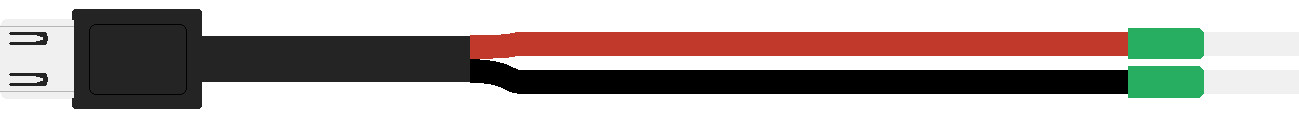
\includegraphics[width=\linewidth]{images/UsbCable.jpg}%
{\captionof{figure}{Schematic representation of the USB cable}}% Take note of the surrounding {} to encapsulate special format settings

Since an \hrefIdx{https://www.espressif.com/en/products/hardware/esp32-devkitc/overview}{ESP32-DevKitC} is used in the Open3DScanner, it is necessary to supply it with power via the Micro-USB-B socket.%

The cable diameter for the USB cable is not specified as any USB cable can be used to power the ESP32. The available USB cables on the market have different cable diameters, but it is not necessary to buy a special cable.%

\paragraph{Bi-Color LED Cable}\mbox{}\\%

\sideTabularx[Bi-color LED cable characteristics]{%
	\rowcolors{2}{tableLineTwo}{tableLineOne}% specify rowcolors in tabularx style
	\begin{tabularx} {\marginparwidth} {>{\rowmac \hsize=\hsize}X>{\rowmac \hsize=\hsize}X<{\clearrow}}%
		\tabularxHeader%
		Characteristic & Value\\%
		Quantity & 1\\%
		Wire Gauge & \SI{0.2}{\milli\meter\squared}\\%
		Length & \SI{11}{\centi\meter}\\%
		End A Connector & 3-Pin Dupont\\%
		End B Connector & 3-Pin Dupont\\%
		End A connects & PCB contact D1\\%
		End B connects & Bi-color LED\\%
	\end{tabularx}%
}%

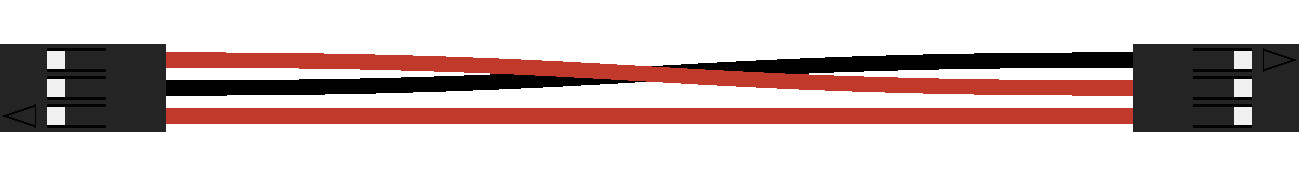
\includegraphics[width=\linewidth]{images/DualColorLedCable.jpg}%
{\captionof{figure}{Schematic representation of the bi-color LED cable}}% Take note of the surrounding {} to encapsulate special format settings

The bi-color LED is plugged directly into the Dupont connector.%

When assembling this cable it is important to pay attention to the cable assignment. The two plugs are not connected identically.%

\clearpage%

\paragraph{Encoder Cable}\mbox{}\\%

\sideTabularx[Encoder cable characteristics]{%
	\rowcolors{2}{tableLineTwo}{tableLineOne}% specify rowcolors in tabularx style
	\begin{tabularx} {\marginparwidth} {>{\rowmac \hsize=\hsize}X>{\rowmac \hsize=\hsize}X<{\clearrow}}%
		\tabularxHeader%
		Characteristic & Value\\%
		Quantity & 1\\%
		Wire Gauge & \SI{0.2}{\milli\meter\squared}\\%
		Length & \SI{15}{\centi\meter}\\%
		End A Connector & 3-Pin Dupont\\%
		End B Connector & 2$\times$3-Pin Dupont\\%
		End A connects & PCB contact SW1\\%
		End B connects & Rotary Encoder\\%
	\end{tabularx}%
}%

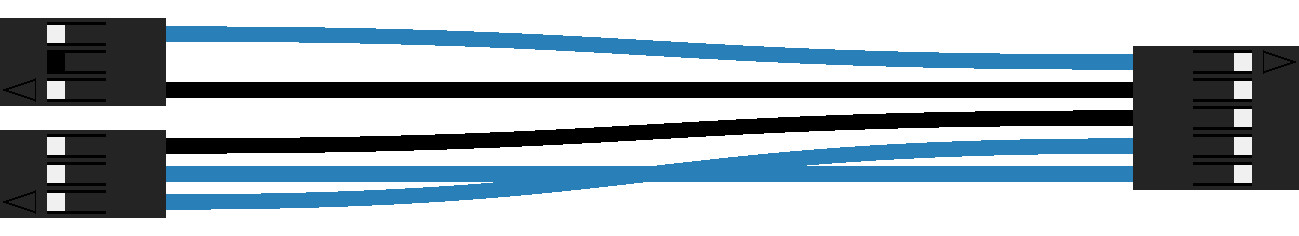
\includegraphics[width=\linewidth]{images/EncoderCable.jpg}%
{\captionof{figure}{Schematic representation of the encoder cable}}% Take note of the surrounding {} to encapsulate special format settings

As with the bi-color LED, the cable for the encoder is connected directly to the component. However, there is a special aspect here which is given by the pin layout of the encoder used.%

The pins of the encoder are arranged in two rows (2 + 3). The pins of the 2-series are arranged like a 3-series, where the middle pin is missing. For this reason, two 3-pin Dupont housings are used on the component side, where one space remains unoccupied.%

\paragraph{Display Cable}\mbox{}\\%

\sideTabularx[Display cable characteristics]{%
	\rowcolors{2}{tableLineTwo}{tableLineOne}% specify rowcolors in tabularx style
	\begin{tabularx} {\marginparwidth} {>{\rowmac \hsize=\hsize}X>{\rowmac \hsize=\hsize}X<{\clearrow}}%
		\tabularxHeader%
		Characteristic & Value\\%
		Quantity & 1\\%
		Wire Gauge & \SI{0.2}{\milli\meter\squared}\\%
		Length & \SI{15}{\centi\meter}\\%
		End A Connector & 8-Pin Dupont\\%
		End B Connector & 8-Pin Dupont\\%
		End A connects & PCB contact DS1\\%
		End B connects & Display\\%
	\end{tabularx}%
}%

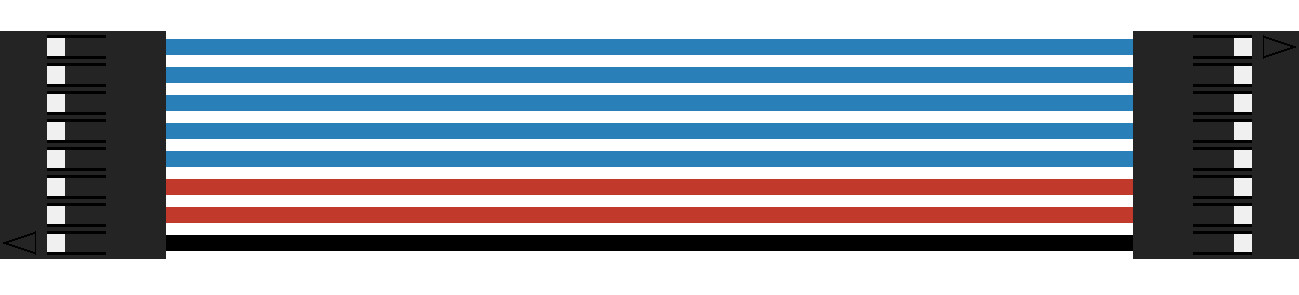
\includegraphics[width=\linewidth]{images/DisplayCable.jpg}%
{\captionof{figure}{Schematic representation of the display cable}}% Take note of the surrounding {} to encapsulate special format settings

Since the used display is mounted on a printed circuit board, the cable is connected to the two pin headers on the display and the PCB.

\section{Assembly the Open3DScanner}%
\label{sec:assembly}
After all the necessary preparatory work has been done, the actual instructions for building the Open3DScanner follow.%

Each individual step is illustrated by an figure. In addition, each step is provided with a short instruction and, if useful, further tips, warnings and notes are given.%

At each step all used components are listed. If these partially assembled parts are subsequently used in further steps, they will not be listed again.%

At the end there are further illustrations, which contain exact dimensions and orientations of parts.%
\clearpage%

% STEP 1
\sideTabularx[Required parts for step 1]{%
	\rowcolors{2}{tableLineTwo}{tableLineOne}% specify rowcolors in tabularx style
	\begin{tabularx} {\marginparwidth} {>{\rowmac \hsize=1.5\hsize}X>{\rowmac \hsize=0.5\hsize}X<{\clearrow}}%
		\tabularxHeader%
		Part & Quantity\\%
		Rotor-Stand & 1\\%
		Passive-Stand & 1\\%
		625ZZ Bearing & 2\\%
	\end{tabularx}%
}%

\marginInfo*[Instructions]{Press one bearing into each of the openings provided in the upper area of the printed parts. The bearings should be flush with the surface of the printed parts.}%

\marginTips*[Tip]{If the opening for the bearings is a tad too tight, you can use pliers to press the bearings into the opening. In this case a piece of fabric or tissue should be placed between the pliers and the components to avoid craters and deformation.}%

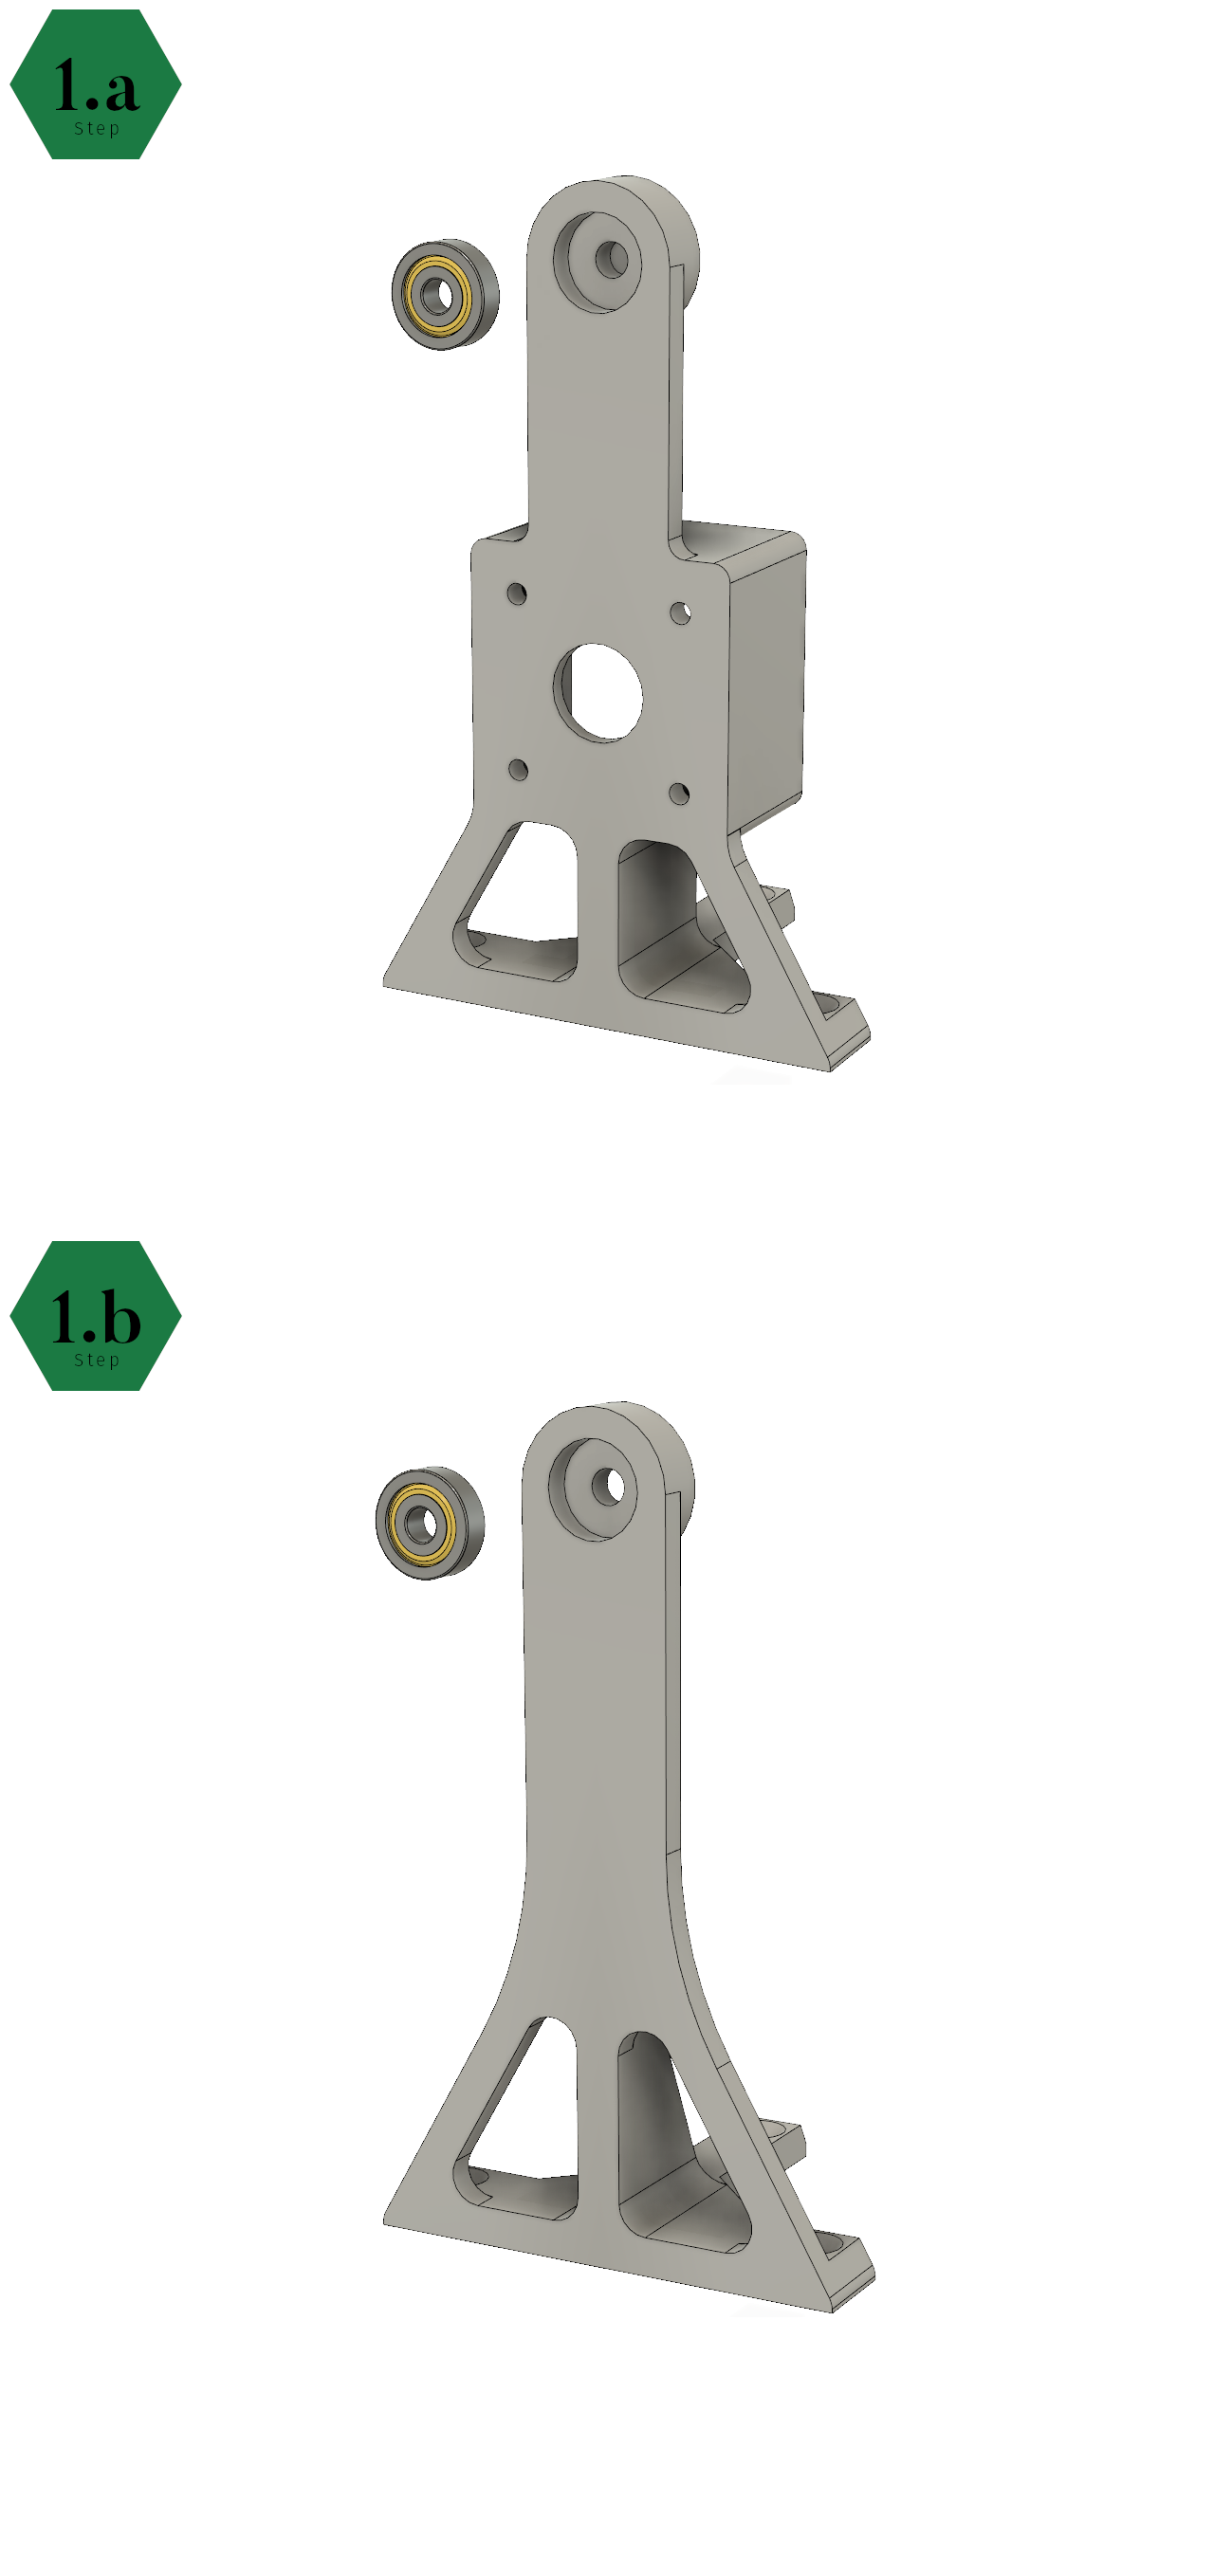
\includegraphics{images/Assembly1.png}%
{\captionof{figure}{Step 1 of the Open3DScanner assembly}}
\clearpage%

% STEP 2&3
\sideTabularx[Required parts for step 2]{%
	\rowcolors{2}{tableLineTwo}{tableLineOne}% specify rowcolors in tabularx style
	\begin{tabularx} {\marginparwidth} {>{\rowmac \hsize=1.5\hsize}X>{\rowmac \hsize=0.5\hsize}X<{\clearrow}}%
		\tabularxHeader%
		Part & Quantity\\%
		Nema 17 Stepper Motor & 2\\%
		Nema 17 Damper & 2\\%
		M3$\times$6 & 4\\%
	\end{tabularx}%
}%

\marginInfo*[Instructions]{Screw the dampers to the stepper motors.}%

\marginTips*[Tip]{The orientation of the dampers does not matter, it is only important that the side with the threads points away from the stepper motor.}%

\sideTabularx[Required parts for step 3]{%
	\vspace{2.65cm}%
	\rowcolors{2}{tableLineTwo}{tableLineOne}% specify rowcolors in tabularx style
	\begin{tabularx} {\marginparwidth} {>{\rowmac \hsize=1.5\hsize}X>{\rowmac \hsize=0.5\hsize}X<{\clearrow}}%
		\tabularxHeader%
		Part & Quantity\\%
		M3$\times$8 & 2\\%
	\end{tabularx}%
}%

\marginInfo*[Instructions]{Screw one stepper motor to the Rotor-Stand.}%

\marginCheck*[Check]{Make sure that the cables are pointing downwards to simplify the wiring later on.}%

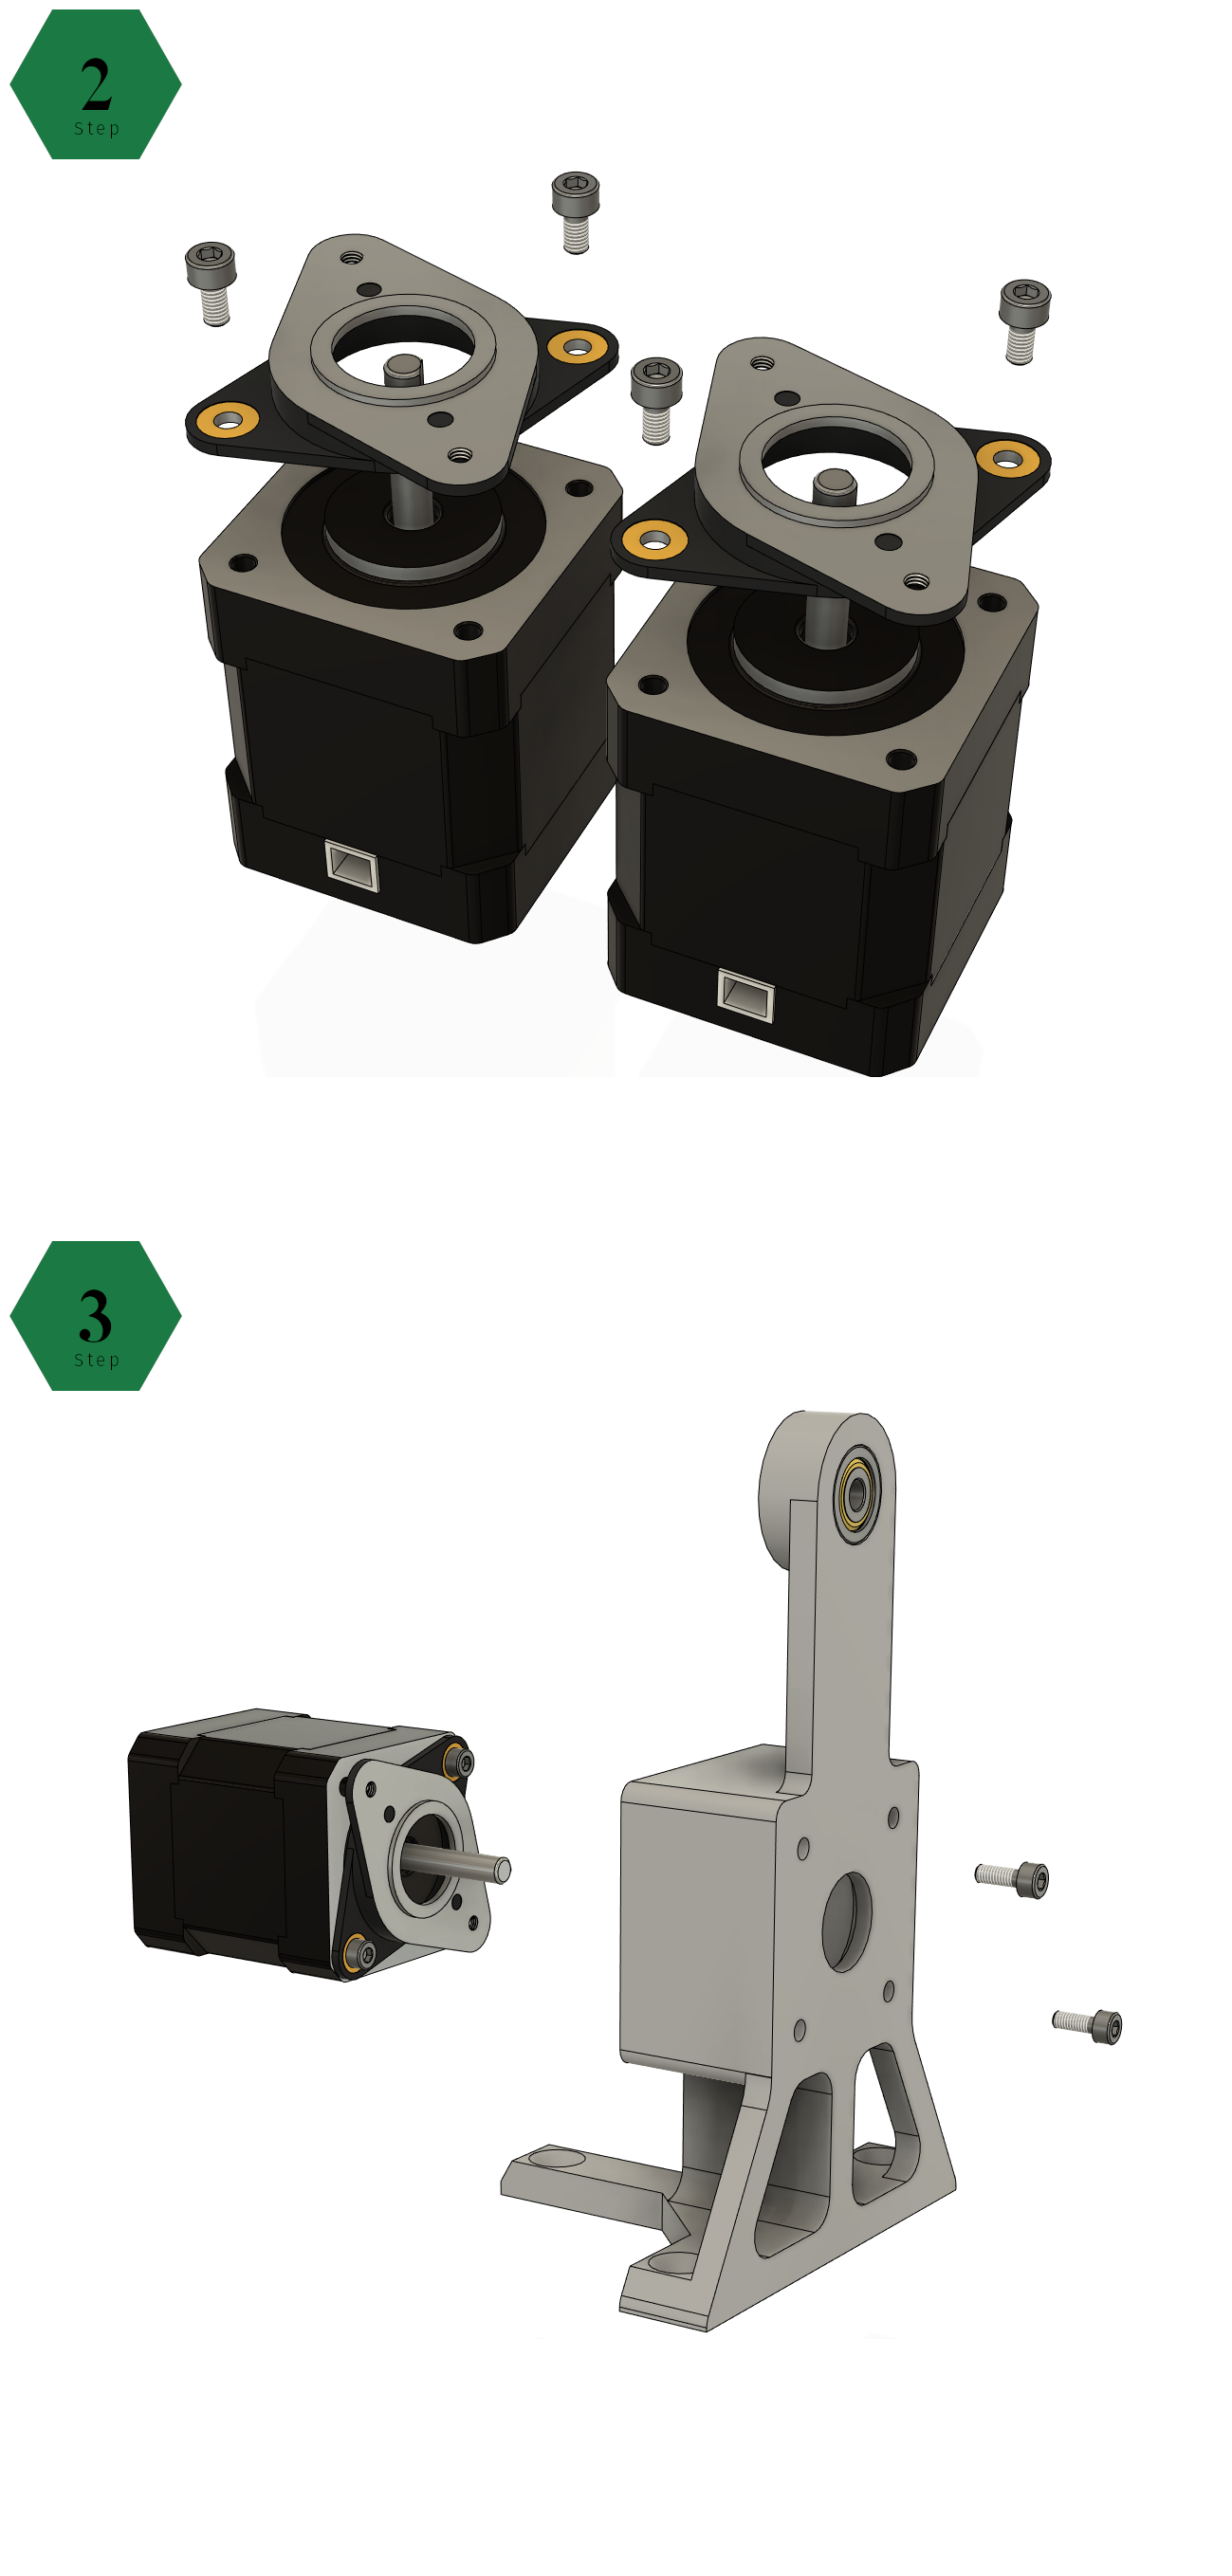
\includegraphics{images/Assembly2.png}%
{\captionof{figure}{Step 2 \& 3 of the Open3DScanner assembly}}
\clearpage%

% STEP 4
\sideTabularx[Required parts for step 4]{%
	\rowcolors{2}{tableLineTwo}{tableLineOne}% specify rowcolors in tabularx style
	\begin{tabularx} {\marginparwidth} {>{\rowmac \hsize=1.5\hsize}X>{\rowmac \hsize=0.5\hsize}X<{\clearrow}}%
		\tabularxHeader%
		Part & Quantity\\%
		Rotor-Gear & 1\\%
		Rotor-Pinion & 1\\%
		\SI{5}{\milli\meter} $\times$ \SI{26}{\milli\meter} Steel Rod & 1\\%
	\end{tabularx}%
}%

\marginInfo*[Instructions]{Press the Rotor-Pinion onto the shaft of the stepper motor. Press the steel rod into the bearing so that it is countersunk as far as possible in the printed part without hindering free rotation. Push the Rotor-Gear onto the steel rod. Use the middle hole of the Rotor-Gear for this.}%

\marginTips*[Tip]{The Rotor-Gear and the steel rod will not be flush. This is not problematic and improves the stability of the assembly in later steps.}%

\marginWarning*[Double check]{The design does not ensure alignment between the two gears. It is intended that the rotor gear is centered on the rotor pinion and protrudes about 1mm on both sides. This must be strictly adhered to in order to allow a smooth movement later on. The connections are so tight that the parts should not slip after alignment.}%

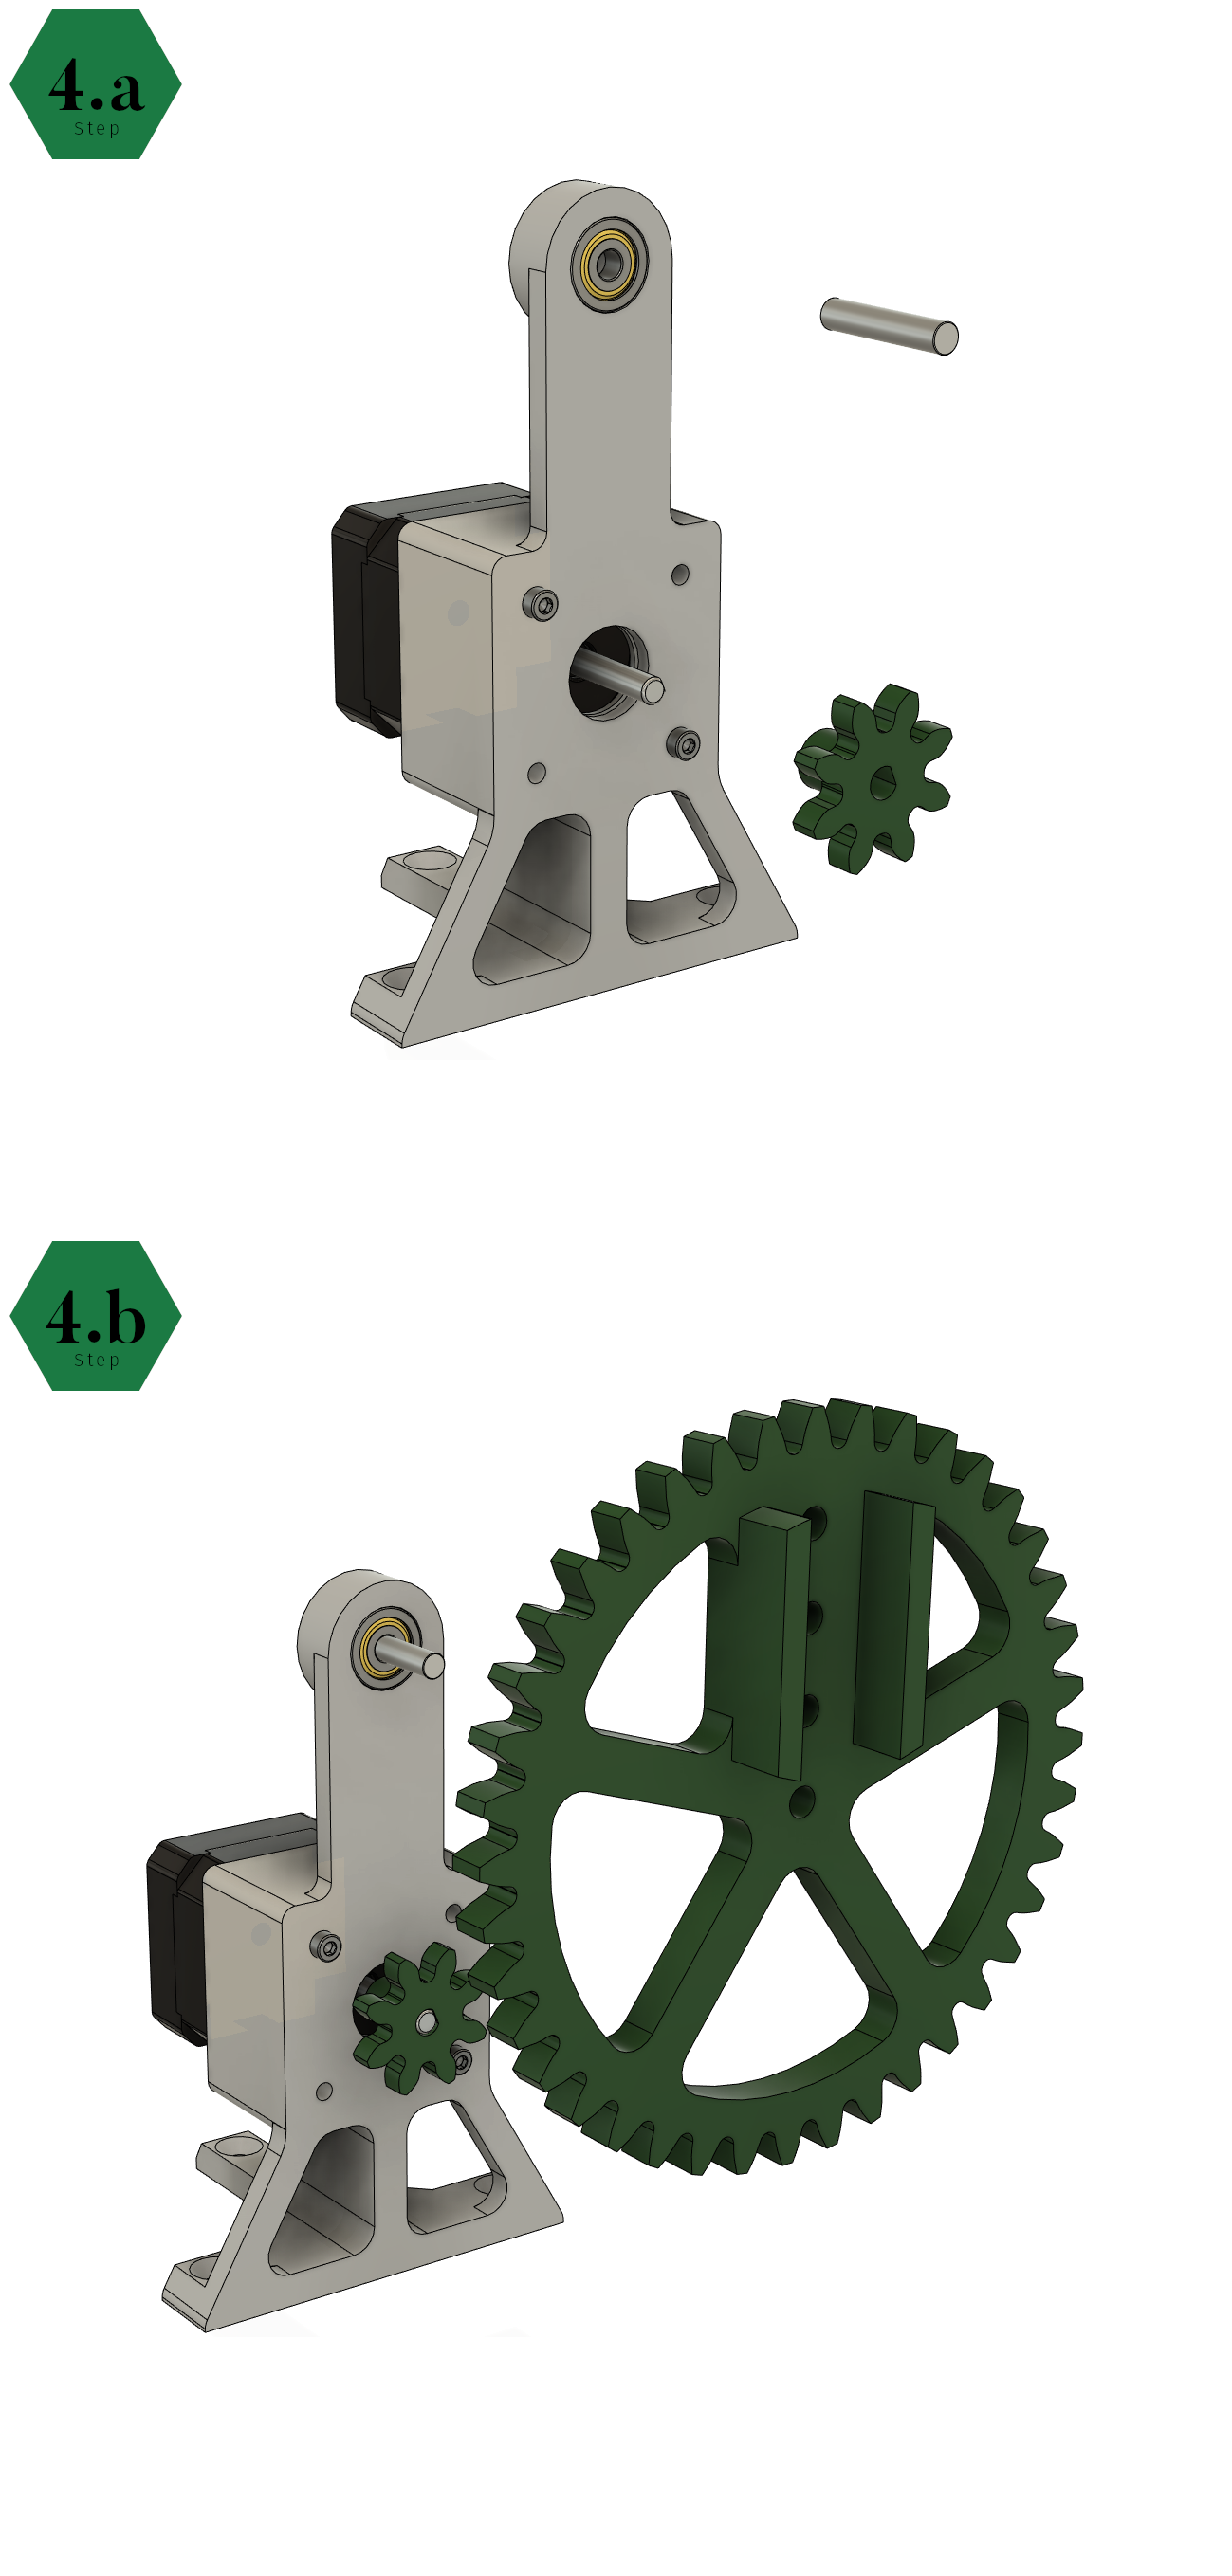
\includegraphics{images/Assembly3.png}%
{\captionof{figure}{Step 4 of the Open3DScanner assembly}}
\clearpage%

% STEP 5
\sideTabularx[Required parts for step 5]{%
	\rowcolors{2}{tableLineTwo}{tableLineOne}% specify rowcolors in tabularx style
	\begin{tabularx} {\marginparwidth} {>{\rowmac \hsize=1.5\hsize}X>{\rowmac \hsize=0.5\hsize}X<{\clearrow}}%
		\tabularxHeader%
		Part & Quantity\\%
		Rotor-Arm & 2\\%
		Turntable-Arm & 1\\%
		\SI{5}{\milli\meter} $\times$ \SI{26}{\milli\meter} Steel Rod & 2\\%
	\end{tabularx}%
}%

\marginInfo*[Instructions]{Press one Rotor-Arm on each end of the Turntable-Arm so that they are flush with the holes. Press a steel rod into each of the holes to firmly join the components together. The steel rods should be flush with the Rotor-Arm on both sides.}%

\marginCheck*[Check]{Make sure that the Turntable-Arm is correctly turned to prevent subsequent disassembly and correction.}%

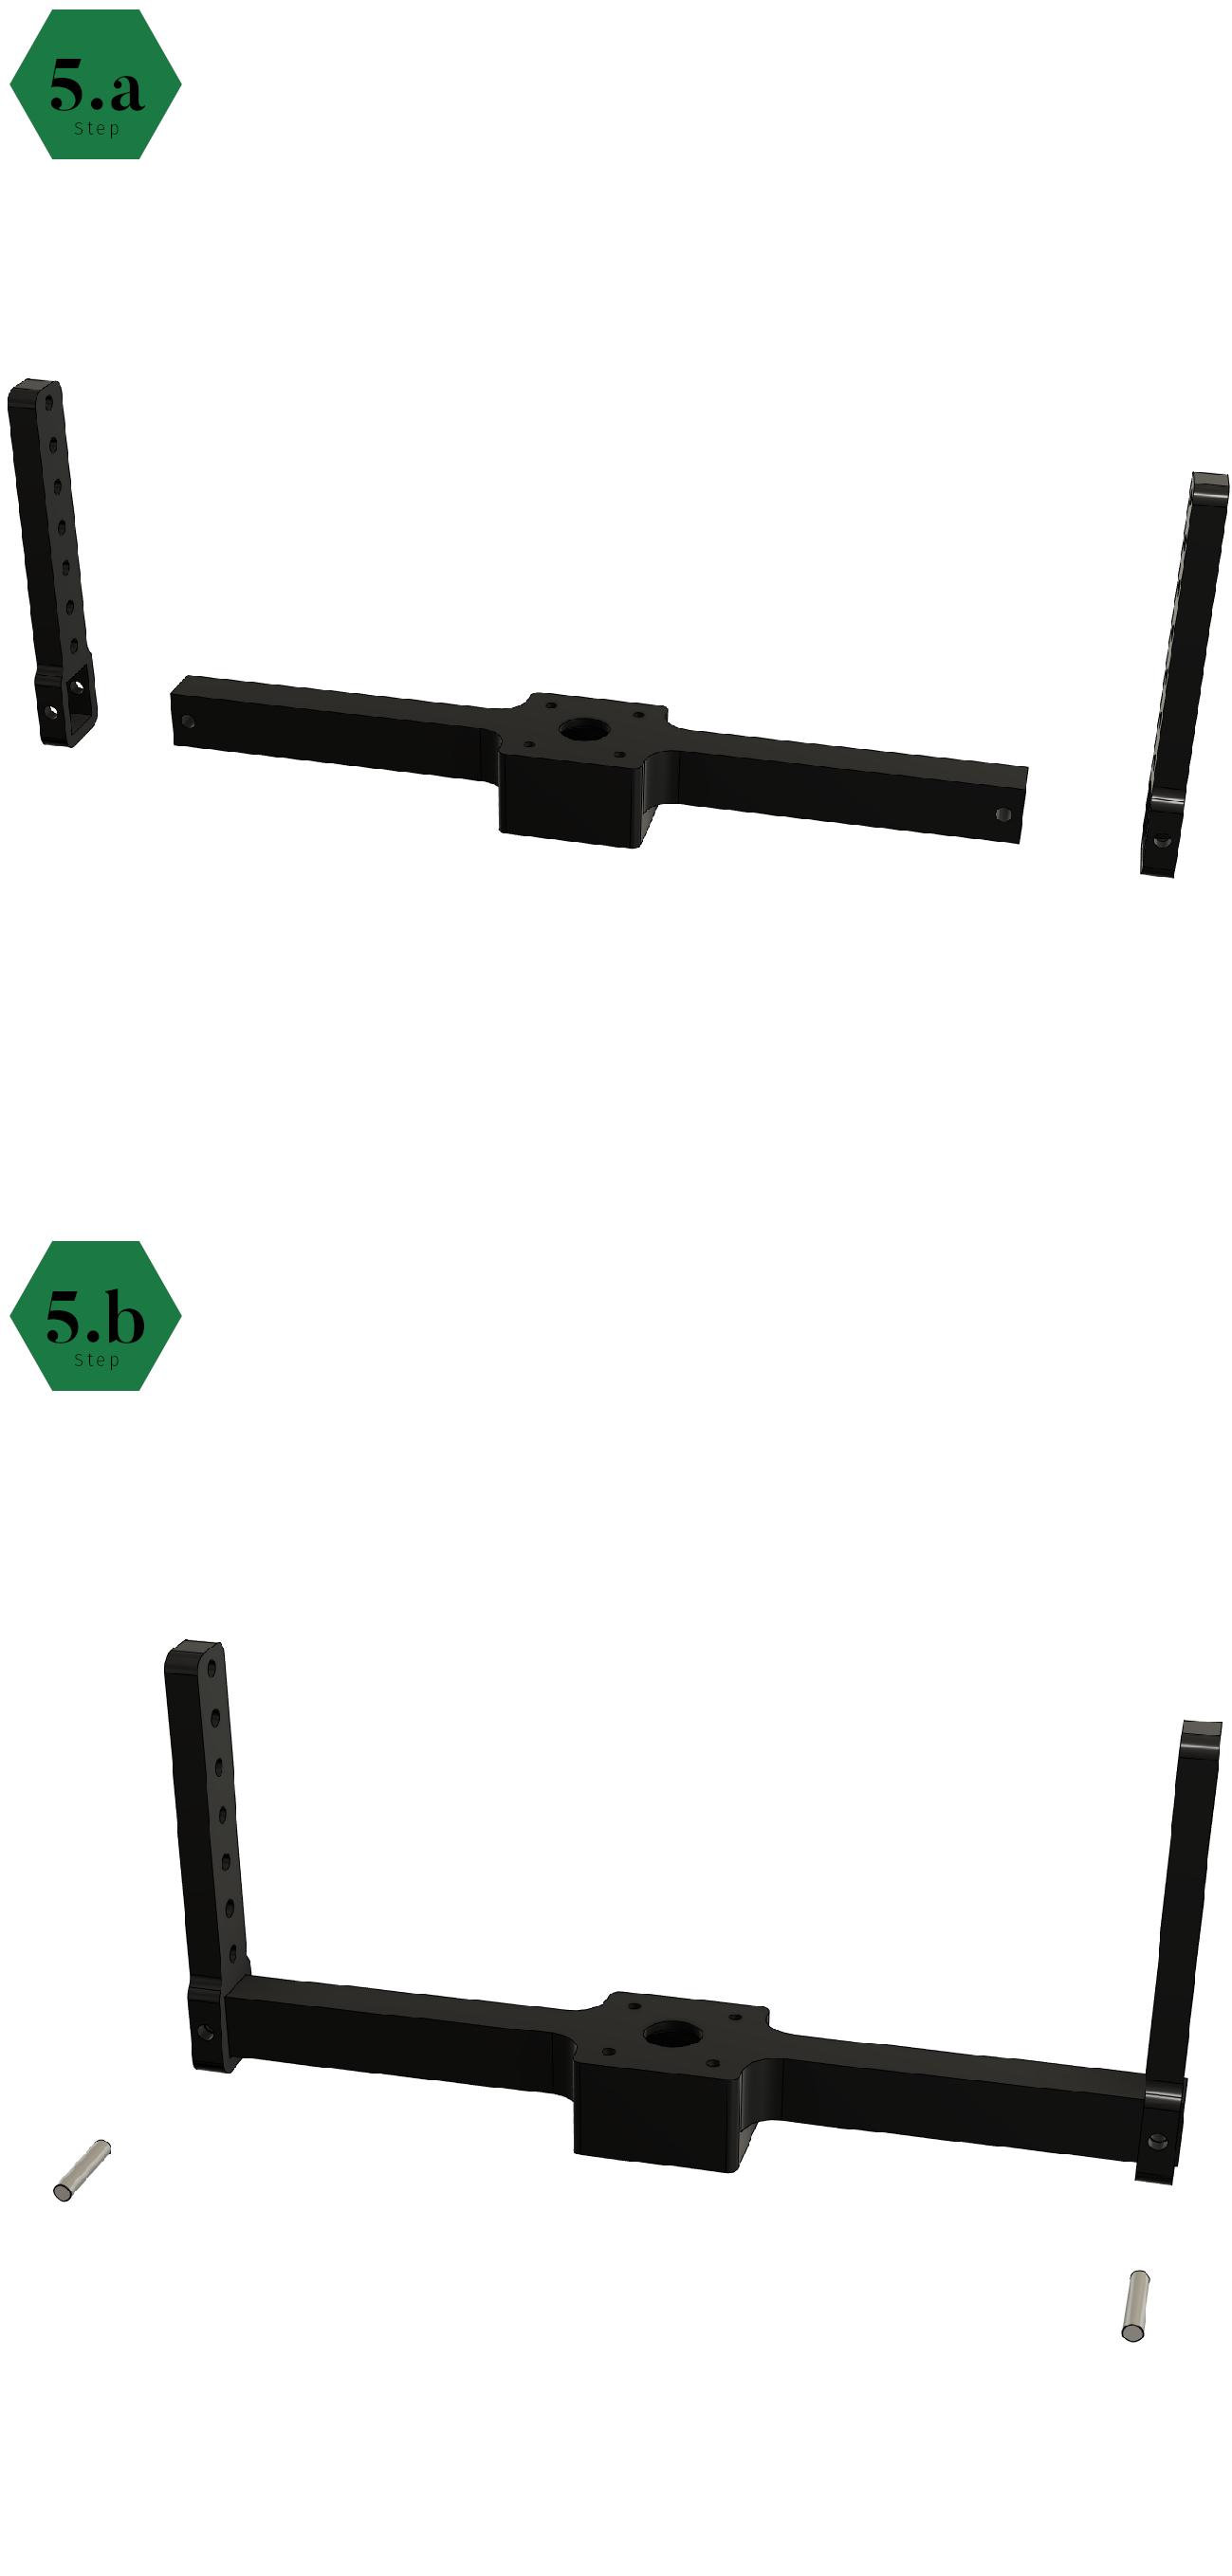
\includegraphics{images/Assembly4.png}%
{\captionof{figure}{Step 5 of the Open3DScanner assembly}}
\clearpage%

% STEP 6 & 7
\sideTabularx[Required parts for step 6]{%
	\rowcolors{2}{tableLineTwo}{tableLineOne}% specify rowcolors in tabularx style
	\begin{tabularx} {\marginparwidth} {>{\rowmac \hsize=1.5\hsize}X>{\rowmac \hsize=0.5\hsize}X<{\clearrow}}%
		\tabularxHeader%
		Part & Quantity\\%
		M3$\times$8 & 2\\%
	\end{tabularx}%
}%

\marginInfo*[Instructions]{Screw the remaining stepper motor to the Turntable-Arm.}%

\sideTabularx[Required parts for step 7]{%
	\vspace{5.7cm}%
	\rowcolors{2}{tableLineTwo}{tableLineOne}% specify rowcolors in tabularx style
	\begin{tabularx} {\marginparwidth} {>{\rowmac \hsize=1.5\hsize}X>{\rowmac \hsize=0.5\hsize}X<{\clearrow}}%
		\tabularxHeader%
		Part & Quantity\\%
		\SI{5}{\milli\meter} $\times$ \SI{26}{\milli\meter} Steel Rod & 1\\%
	\end{tabularx}%
}%

\marginInfo*[Instructions]{Push the steel rod through the upper hole of one Rotor-Arm and then into the outer hole of the Rotor-Gear. The components should be flush with each other and the Rotor-Arm is fixed to the rotor gear by the two jaws.}%

\marginQuestion*[Information]{The Rotor-Arm is additionally fixed by the steel rod, which connects the Rotor-Gear with the Rotor-Stand.}%

\marginCheck*[Check]{Make sure that the motor cables point towards you when the Rotor-Stand is on the left side. This will allow clean wiring.}%

\marginCritical*[Warning]{For accurate alignment of the steel bar, consider the image cutout. The rod must protrude a little bit from the rotor arm, otherwise the rotation of the device will be blocked.}%

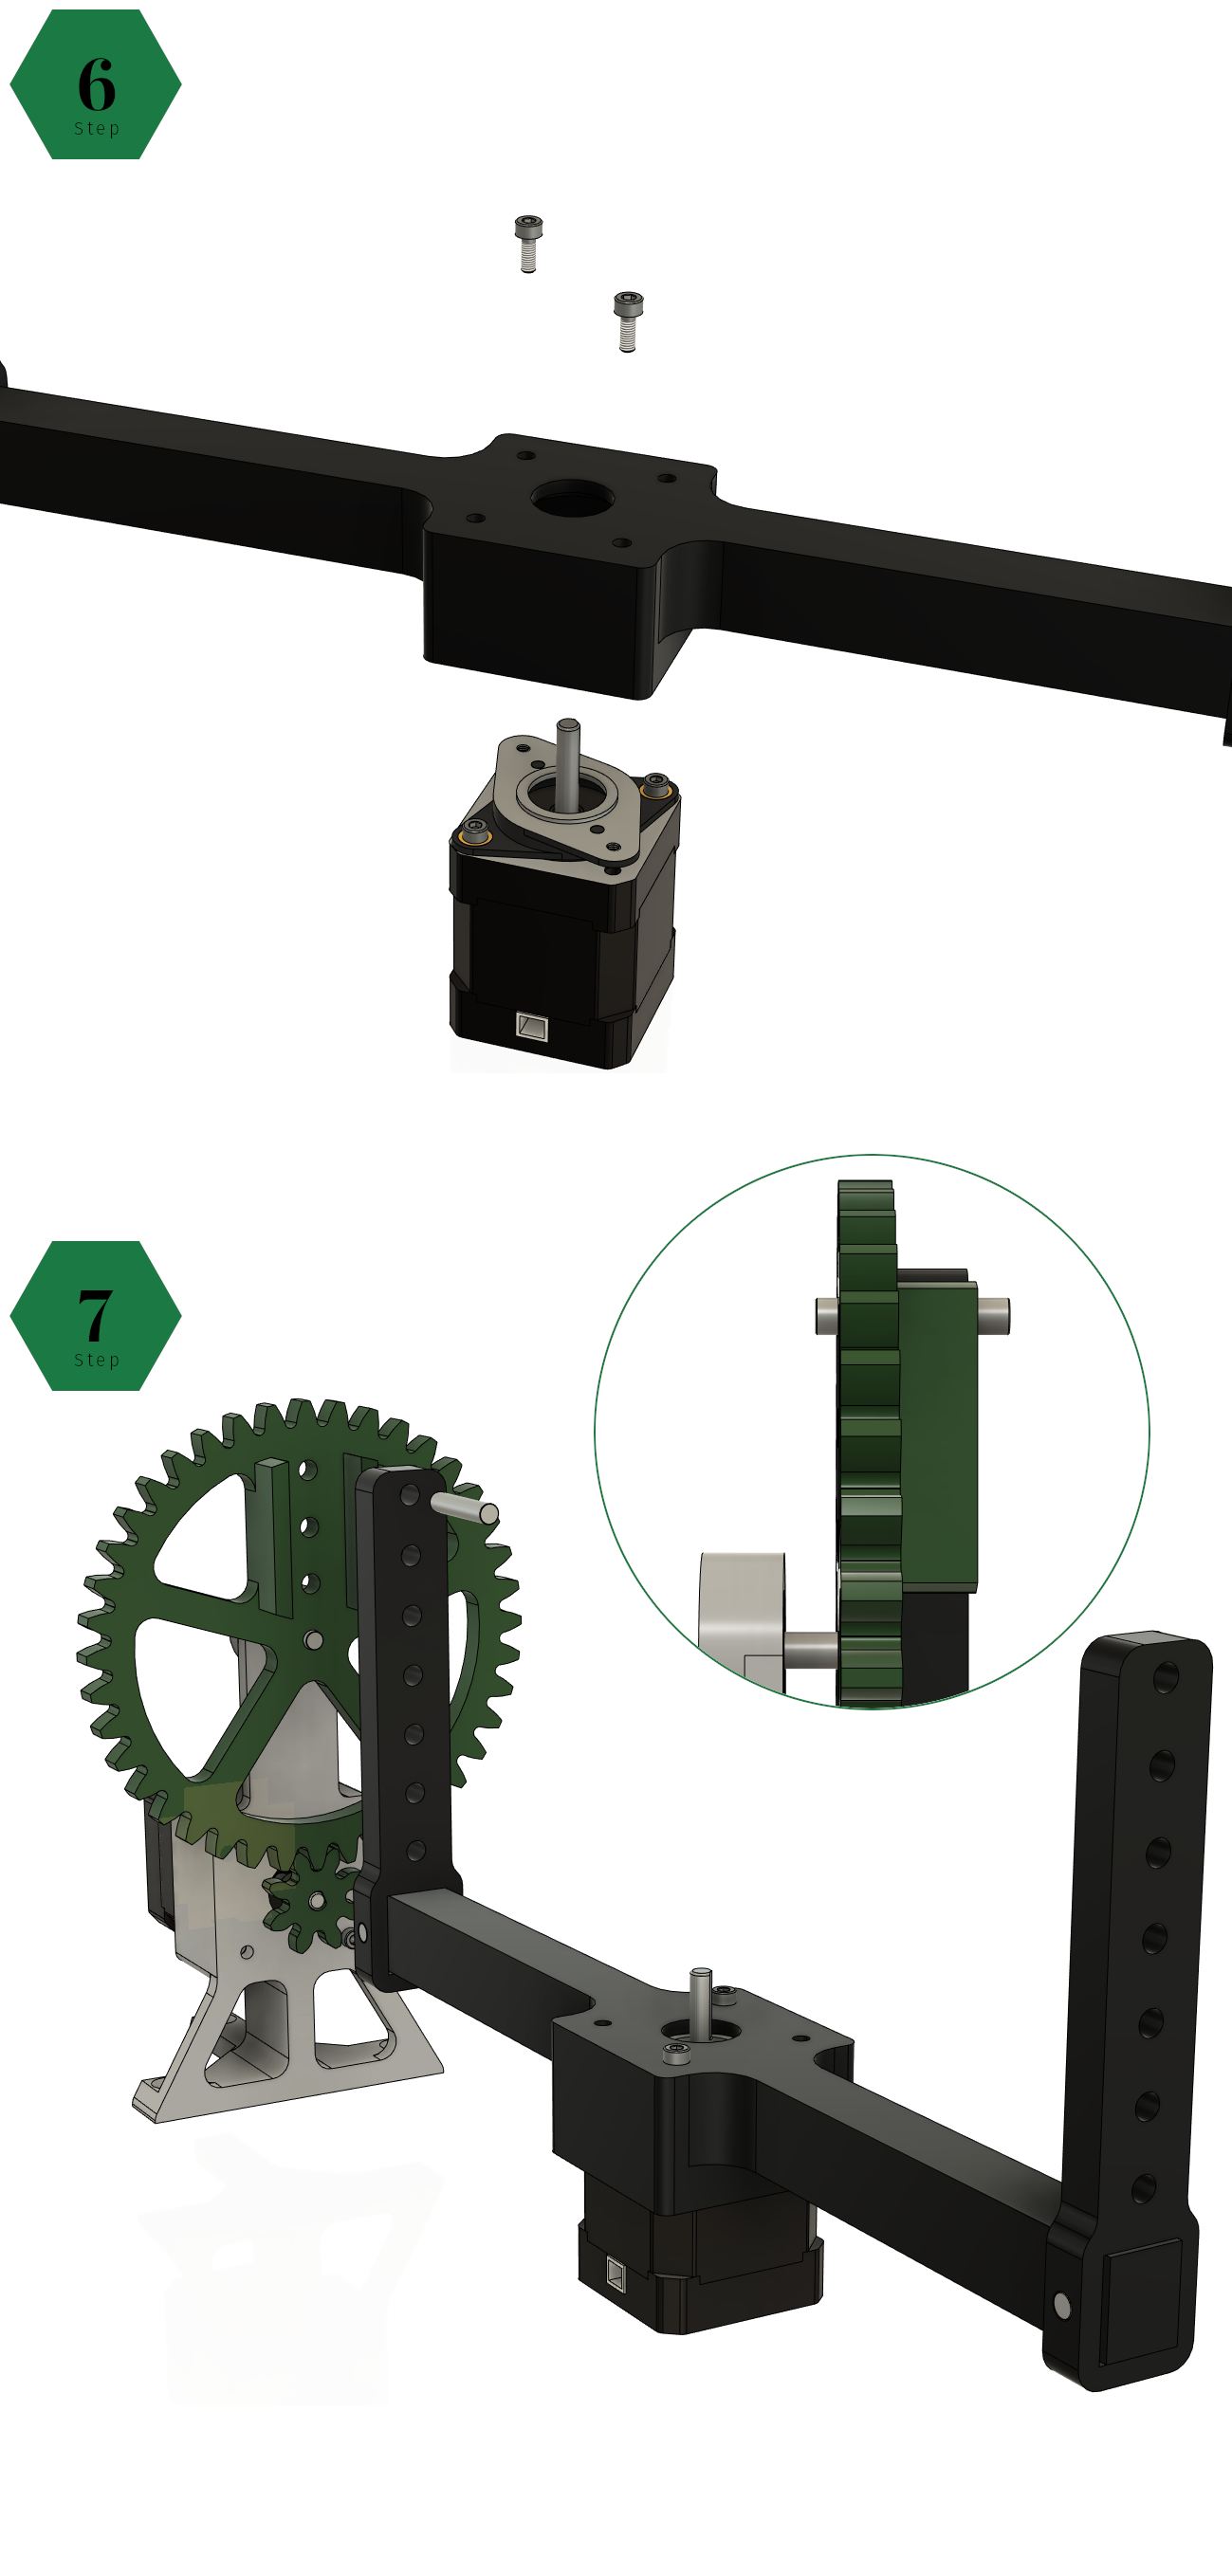
\includegraphics{images/Assembly5.png}%
{\captionof{figure}{Step 6 \& 7 of the Open3DScanner assembly}}
\clearpage%

% STEP 8 & 9
\sideTabularx[Required parts for step 8]{%
	\rowcolors{2}{tableLineTwo}{tableLineOne}% specify rowcolors in tabularx style
	\begin{tabularx} {\marginparwidth} {>{\rowmac \hsize=1.5\hsize}X>{\rowmac \hsize=0.5\hsize}X<{\clearrow}}%
		\tabularxHeader%
		Part & Quantity\\%
		\SI{5}{\milli\meter} $\times$ \SI{26}{\milli\meter} Steel Rod & 1\\%
	\end{tabularx}%
}%

\marginInfo*[Instructions]{Connect the other Rotor-Arm to the bearing in the Passive-Stand. Use the center hole in the Rotor-Arm for this. The rod will be flush with the Rotor-Arm and protrude a bit from the back of the Passive-Stand.}%

\sideTabularx[Required parts for step 9]{%
	\vspace{5.0cm}%
	\rowcolors{2}{tableLineTwo}{tableLineOne}% specify rowcolors in tabularx style
	\begin{tabularx} {\marginparwidth} {>{\rowmac \hsize=1.5\hsize}X>{\rowmac \hsize=0.5\hsize}X<{\clearrow}}%
		\tabularxHeader%
		Part & Quantity\\%
		Turntable-Medium & 1\\%
	\end{tabularx}%
}%

\marginInfo*[Instructions]{Push the Turntable-Medium as far as possible onto the shaft of the stepper motor, which is mounted to the Turntable-Arm.}%

\marginTips*[Tip]{Stabilize the structure by pressing against the bottom of the Turntable-Arm while pushing the Turntable-Medium onto the motor shaft. That way bending and deformation of the parts can be prevented.}%

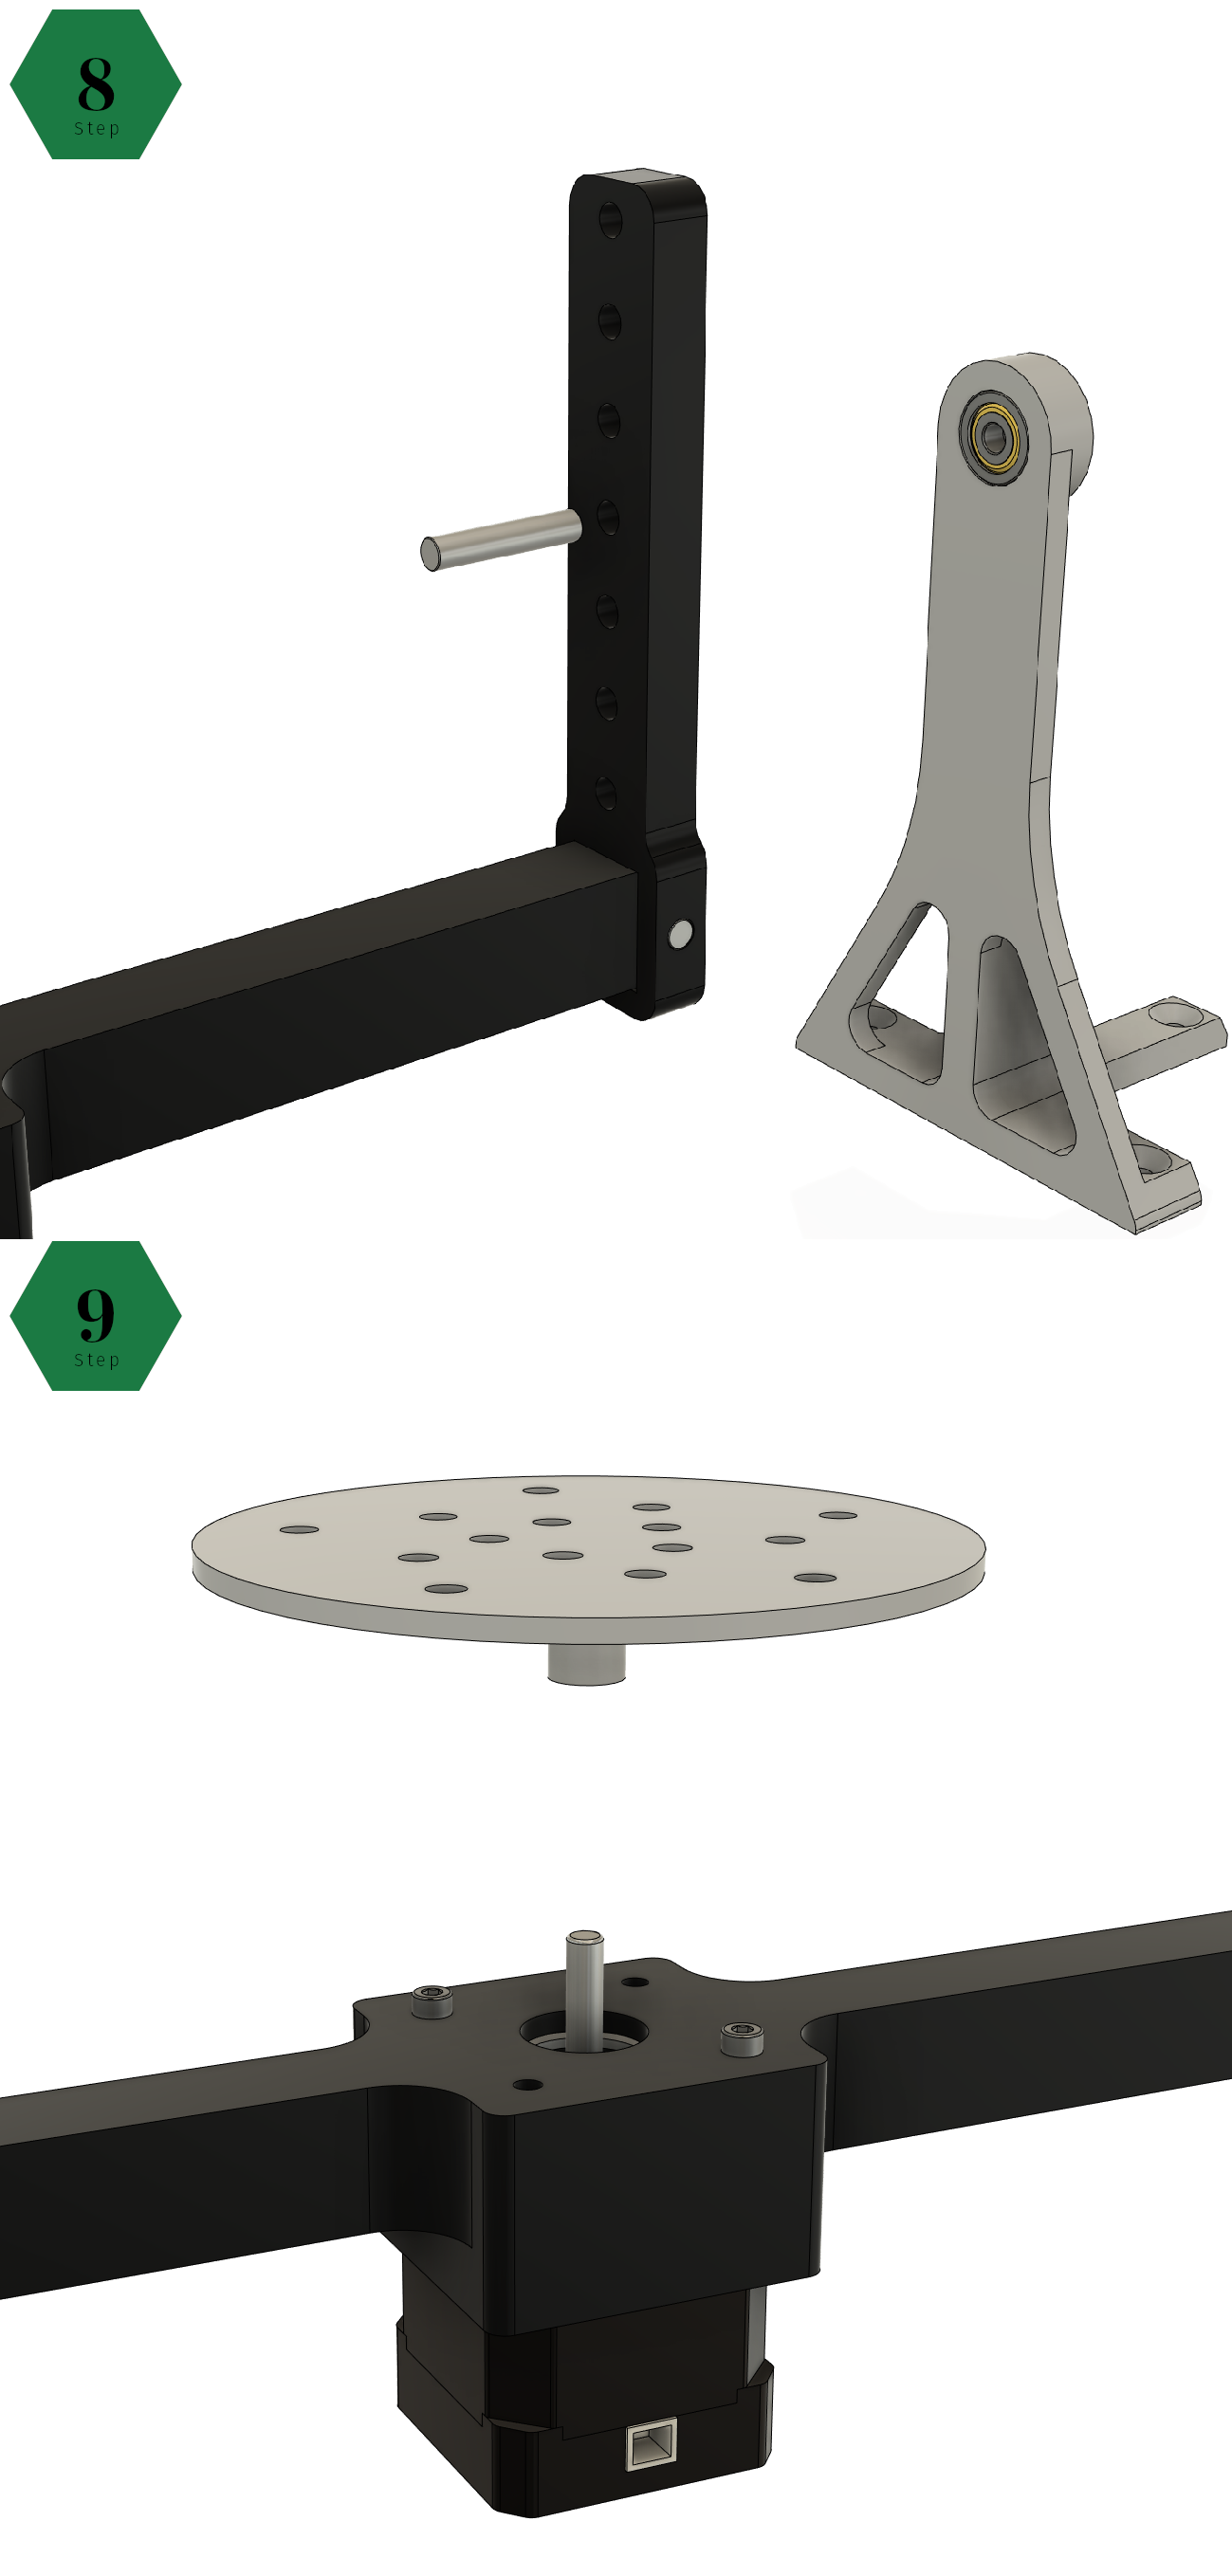
\includegraphics{images/Assembly6.png}%
{\captionof{figure}{Step 8 \& 9 of the Open3DScanner assembly}}
\clearpage%

% STEP 10
\sideTabularx[Required parts for step 10]{%
	\rowcolors{2}{tableLineTwo}{tableLineOne}% specify rowcolors in tabularx style
	\begin{tabularx} {\marginparwidth} {>{\rowmac \hsize=1.5\hsize}X>{\rowmac \hsize=0.5\hsize}X<{\clearrow}}%
		\tabularxHeader%
		Part & Quantity\\%
		Spotlight-Stand & 1\\%
		Spotlight-Frame & 1\\%
		M3$\times$8 & 2\\%
		M3 Nut & 2\\%
	\end{tabularx}%
}%

\marginInfo*[Instructions]{Press the two nuts into the recesses of the Spotlight-Stand. Select two adjacent holes that are at the same height. Next attach the Spotlight-Frame with the Spotlight-Stand. To do this, screw the screws through the holes in the Spotlight-Frame with the nuts on the back of the Spotlight-Stand.}%

\marginTips*[Tip]{Repeat this step up to four times for each spotlight you want to use. The height of the Spotlight frame can be changed by inserting the nuts into other recesses. This allows the illumination for the scans to be changed. The hole in the middle of the lower part of the Spotlight-Frame is for cable routing.}%

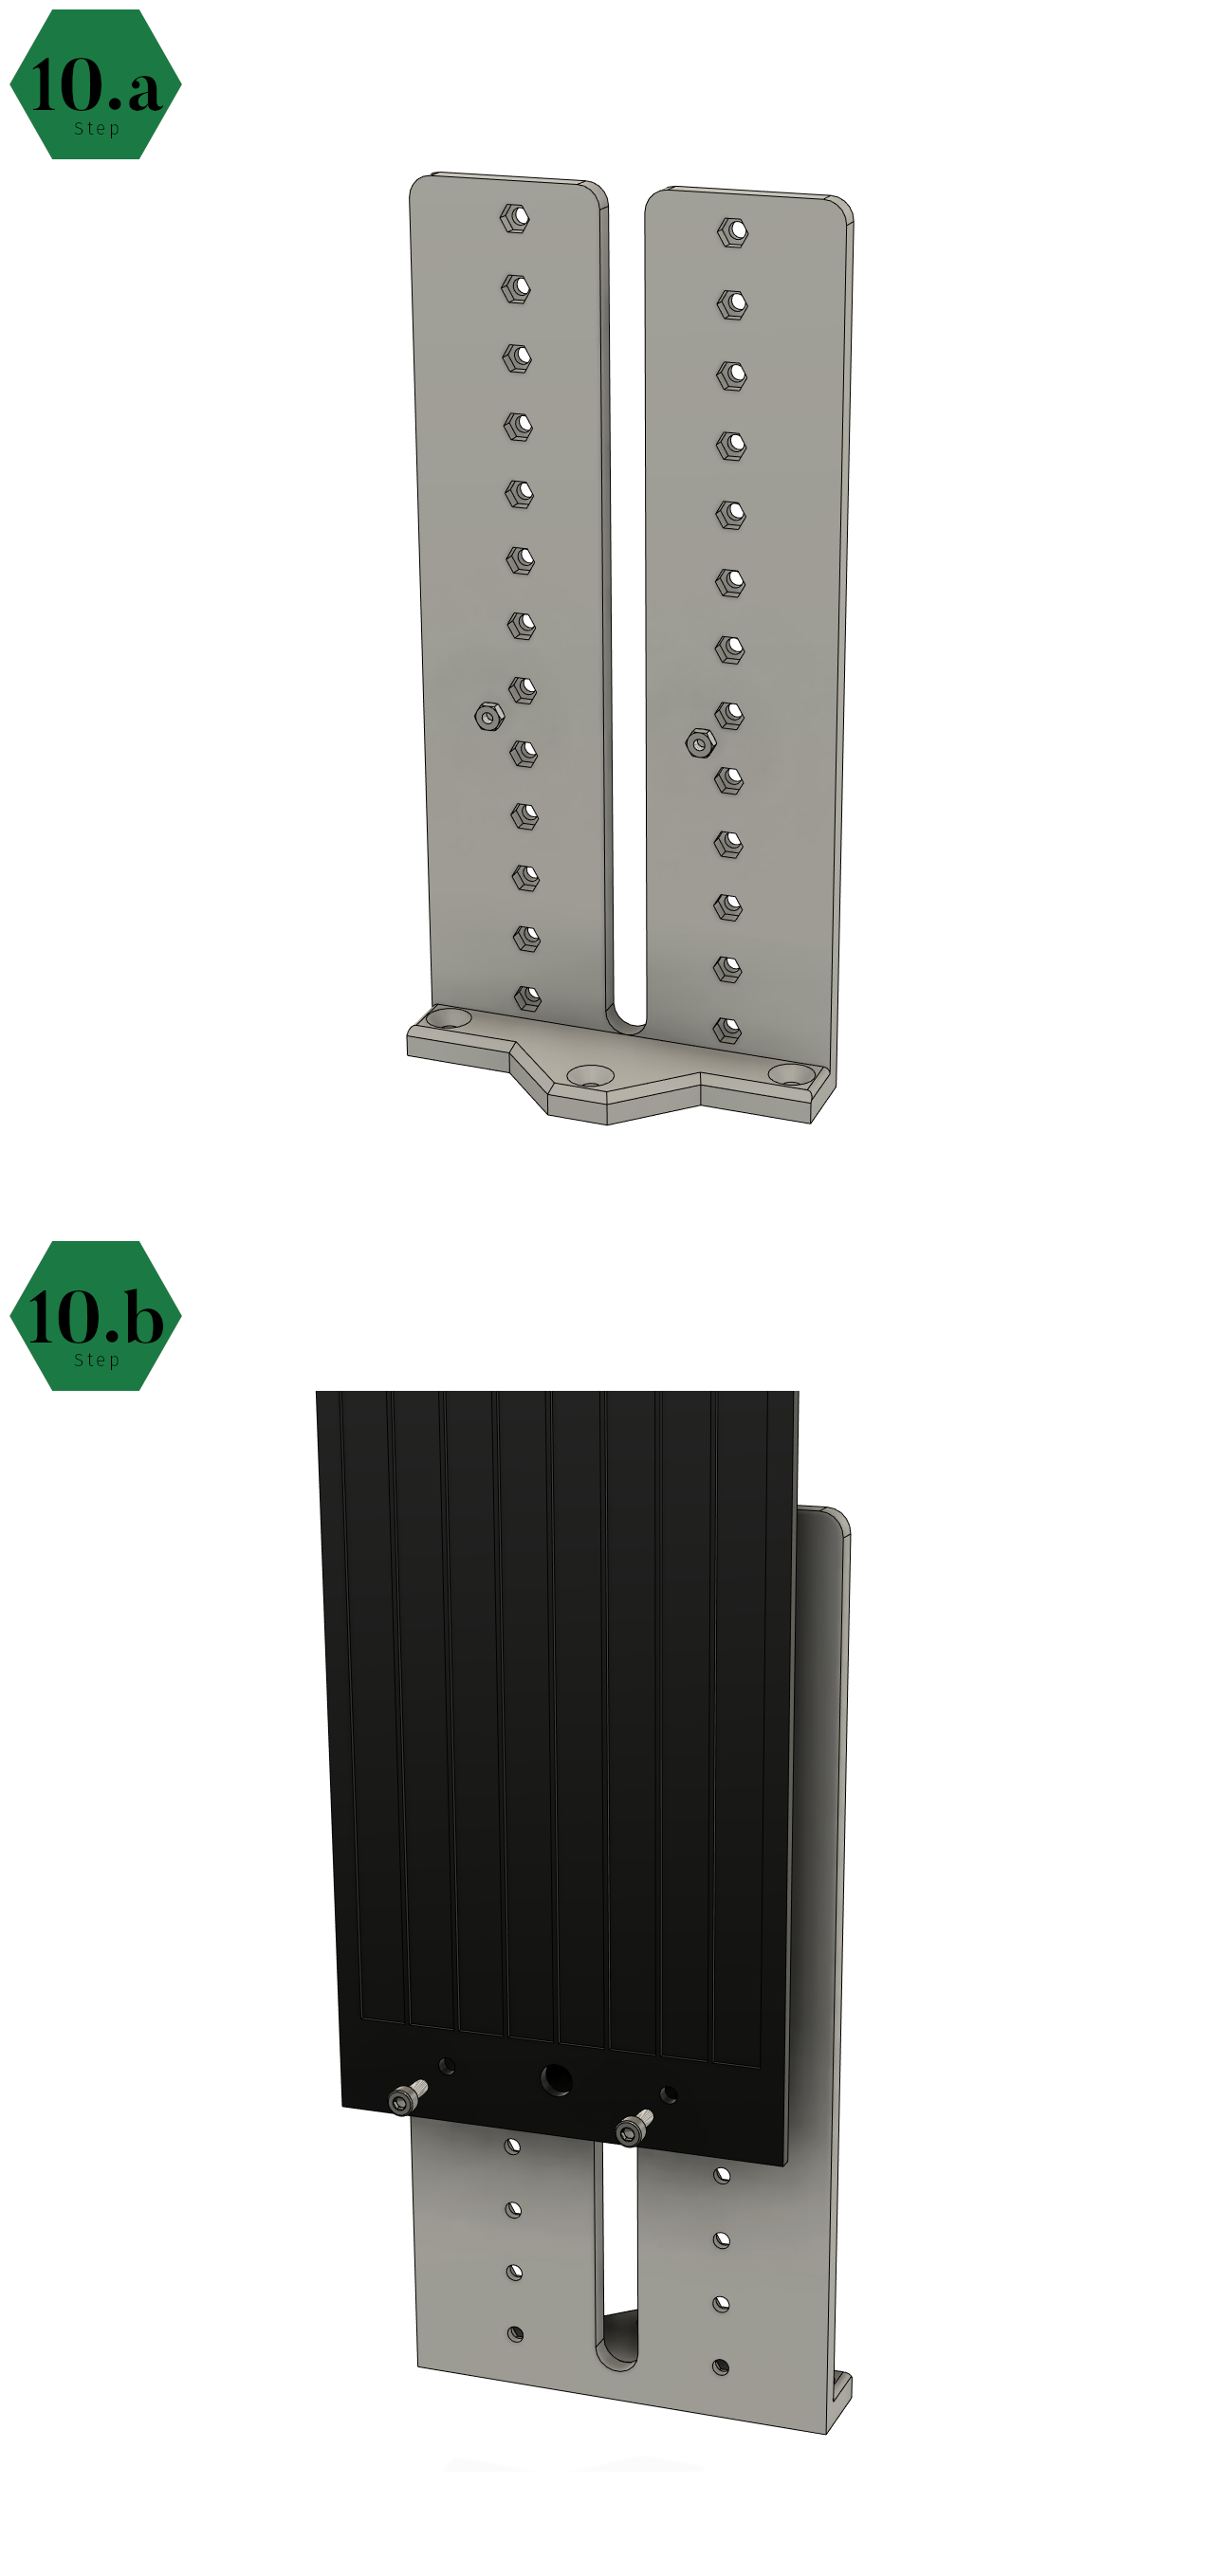
\includegraphics{images/Assembly7.png}%
{\captionof{figure}{Step 10 of the Open3DScanner assembly}}
\clearpage%

% STEP 11
\sideTabularx[Required parts for step 11]{%
	\rowcolors{2}{tableLineTwo}{tableLineOne}% specify rowcolors in tabularx style
	\begin{tabularx} {\marginparwidth} {>{\rowmac \hsize=1.5\hsize}X>{\rowmac \hsize=0.5\hsize}X<{\clearrow}}%
		\tabularxHeader%
		Part & Quantity\\%
		Foot-Holder-Clamp & 4\\%
		\SI{30}{\milli\meter} $\times$ \SI{15}{\milli\meter} Rubber Feet & 4\\%
		M3$\times$20 & 4\\%
		M3 Nut & 4\\%
	\end{tabularx}%
}%

\marginInfo*[Instructions]{Press the nut into the recess on top of the Foot-Holder-Clamp. Then screw the rubber feet with the screw from the bottom to the nut.}%

\marginTips*[Tip]{Repeat this step four times to assemble all feet for the base plate.}%

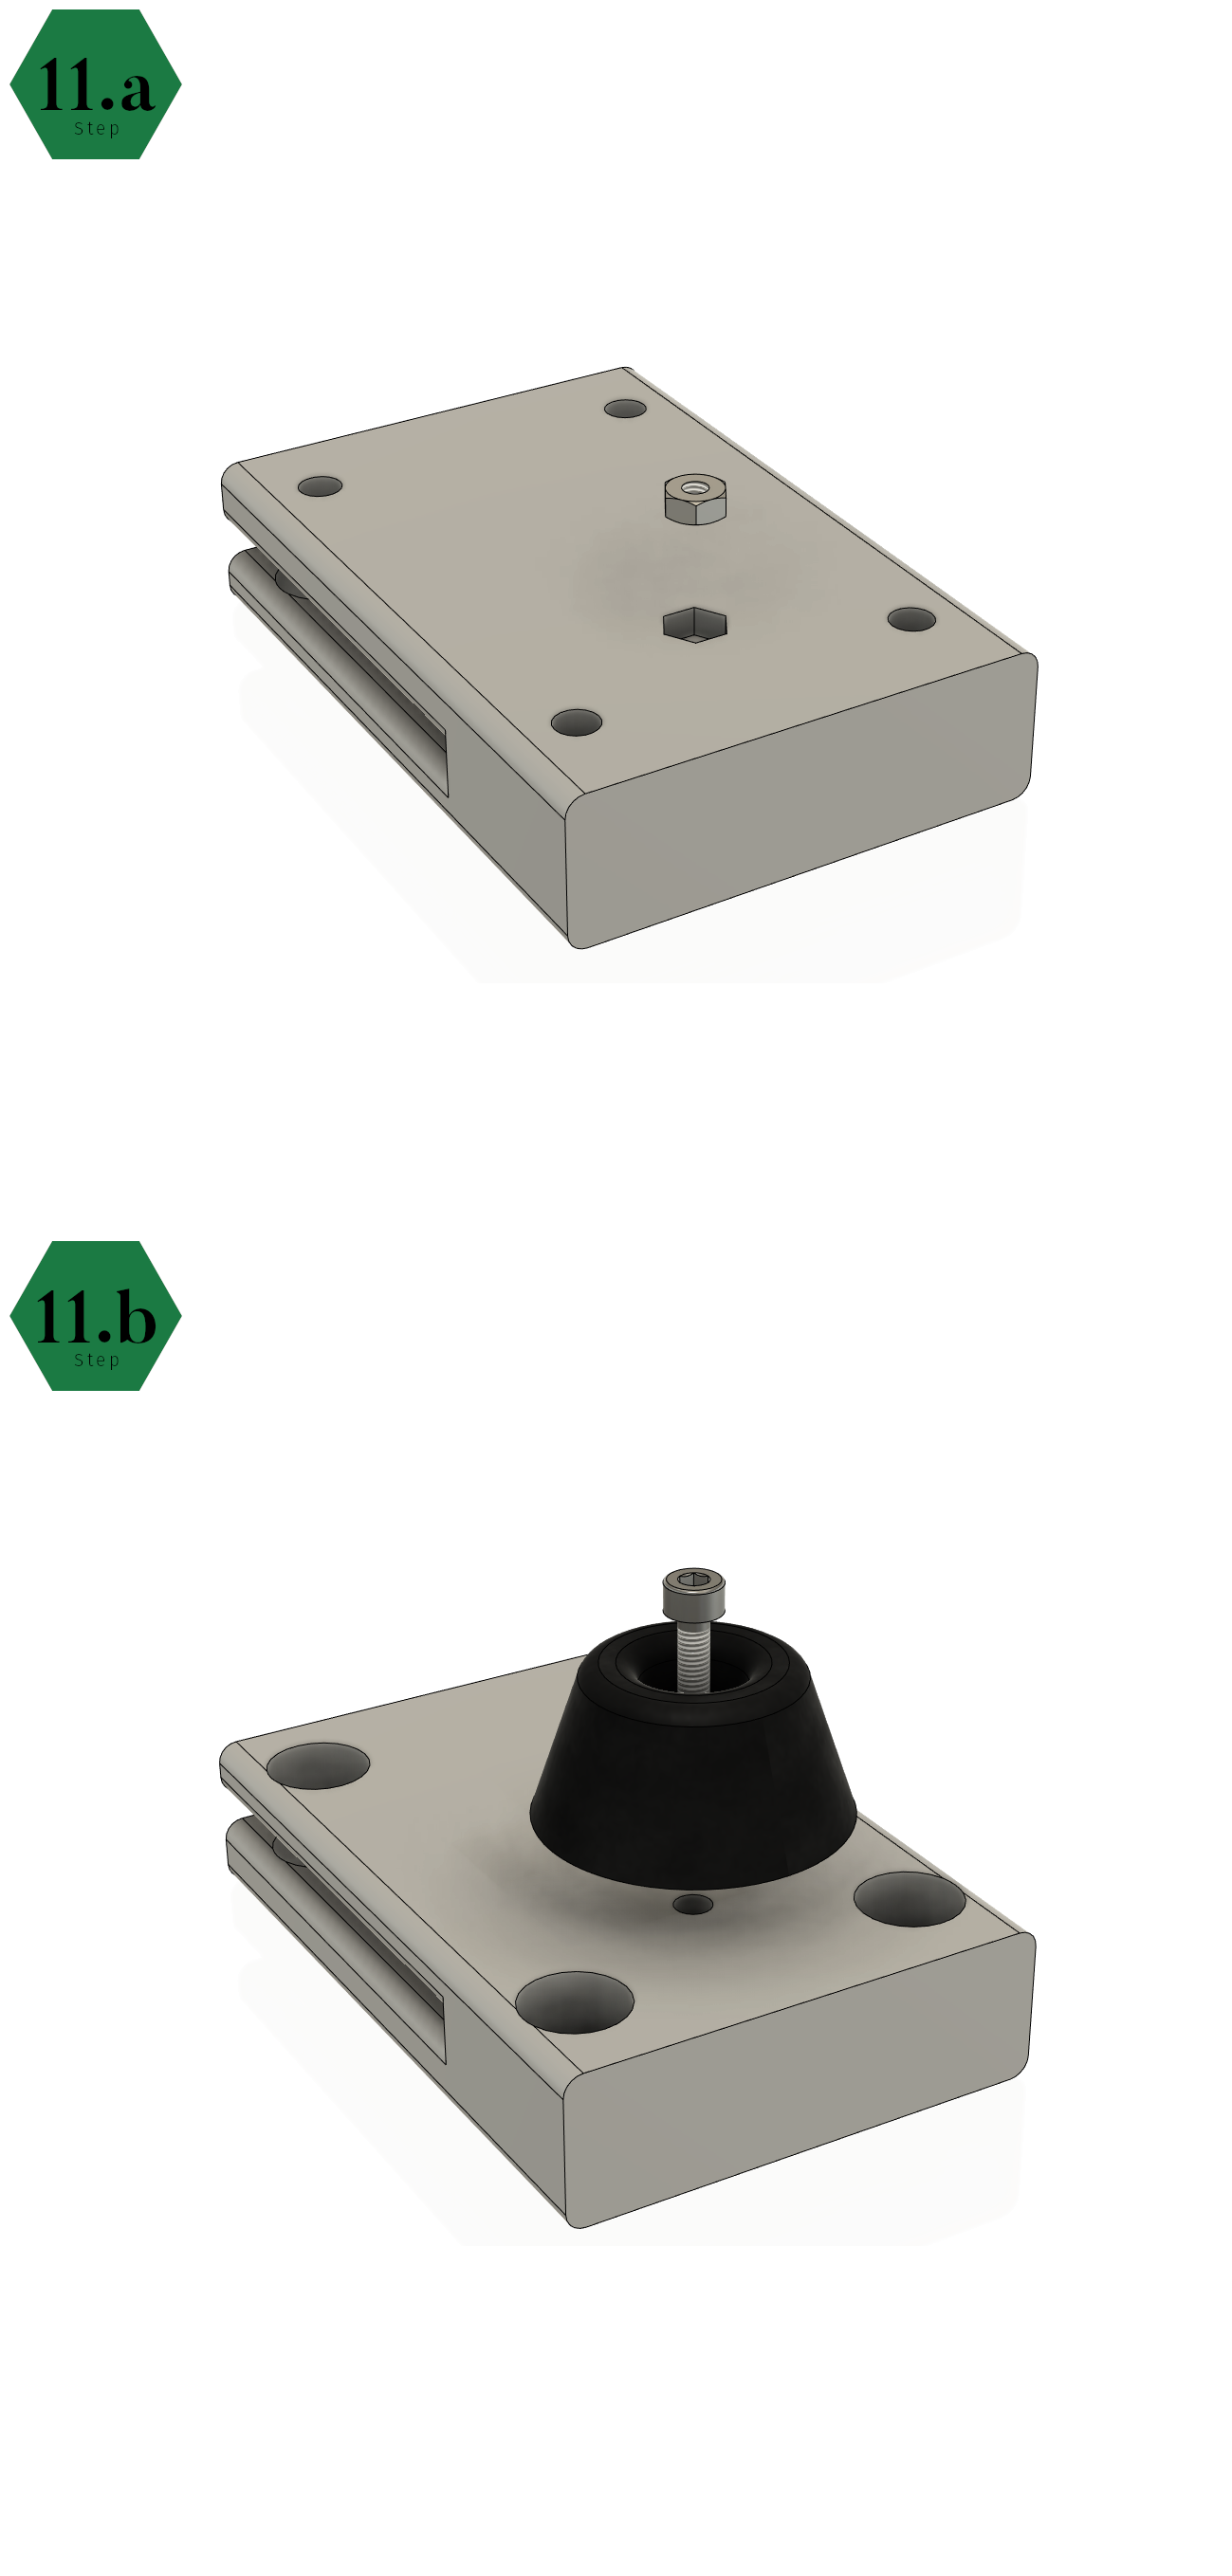
\includegraphics{images/Assembly8.png}%
{\captionof{figure}{Step 11 of the Open3DScanner assembly}}
\clearpage%

% STEP 12
\sideTabularx[Required parts for step 12]{%
	\rowcolors{2}{tableLineTwo}{tableLineOne}% specify rowcolors in tabularx style
	\begin{tabularx} {\marginparwidth} {>{\rowmac \hsize=1.5\hsize}X>{\rowmac \hsize=0.5\hsize}X<{\clearrow}}%
		\tabularxHeader%
		Part & Quantity\\%
		\SI{400}{\milli\meter} $\times$ \SI{550}{\milli\meter} $\times$ \SI{16}{\milli\meter} Wooden Board & 1\\%
		Backplate-Holder & 2\\%
		4.0$\times$16 Countersunk Wood Screwt & 24\\%
	\end{tabularx}%
}%

\marginInfo*[Instructions]{Screw the parts to the wooden board which is used as base plate. Use four screws for each assembled foot and Backplate-Holder. On the underside of the wooden board, mount one foot flush in each corner. The horizontal opening points into the inner area of the plate. The openings of two feet, which are mounted along the long edge of the base plate, face each other. The backplate holders are mounted from the top of the base plate. They are mounted flush in the corners of one of the long edges of the wooden board. The Backplate-Holder inserts have to be parallel to the long edge of the base plate.}%

\marginTips*[Tip]{For scans the backplate is inserted into the Backplate-Holders. When the scanner should be stored the backplate can be slided into the Foot-holder-Clamps to reduce the volume of the scanner.}%

\marginCheck*[Check]{You need to mount four assembled feets and two Backplate-Holder.}%

\marginCritical*[Warning]{Align the components as well as possible at the corners of the wooden board. Otherwise it can happen that the rear panel does not fit properly or that parts cannot be screwed down because the screws on the top and bottom side collide.}%

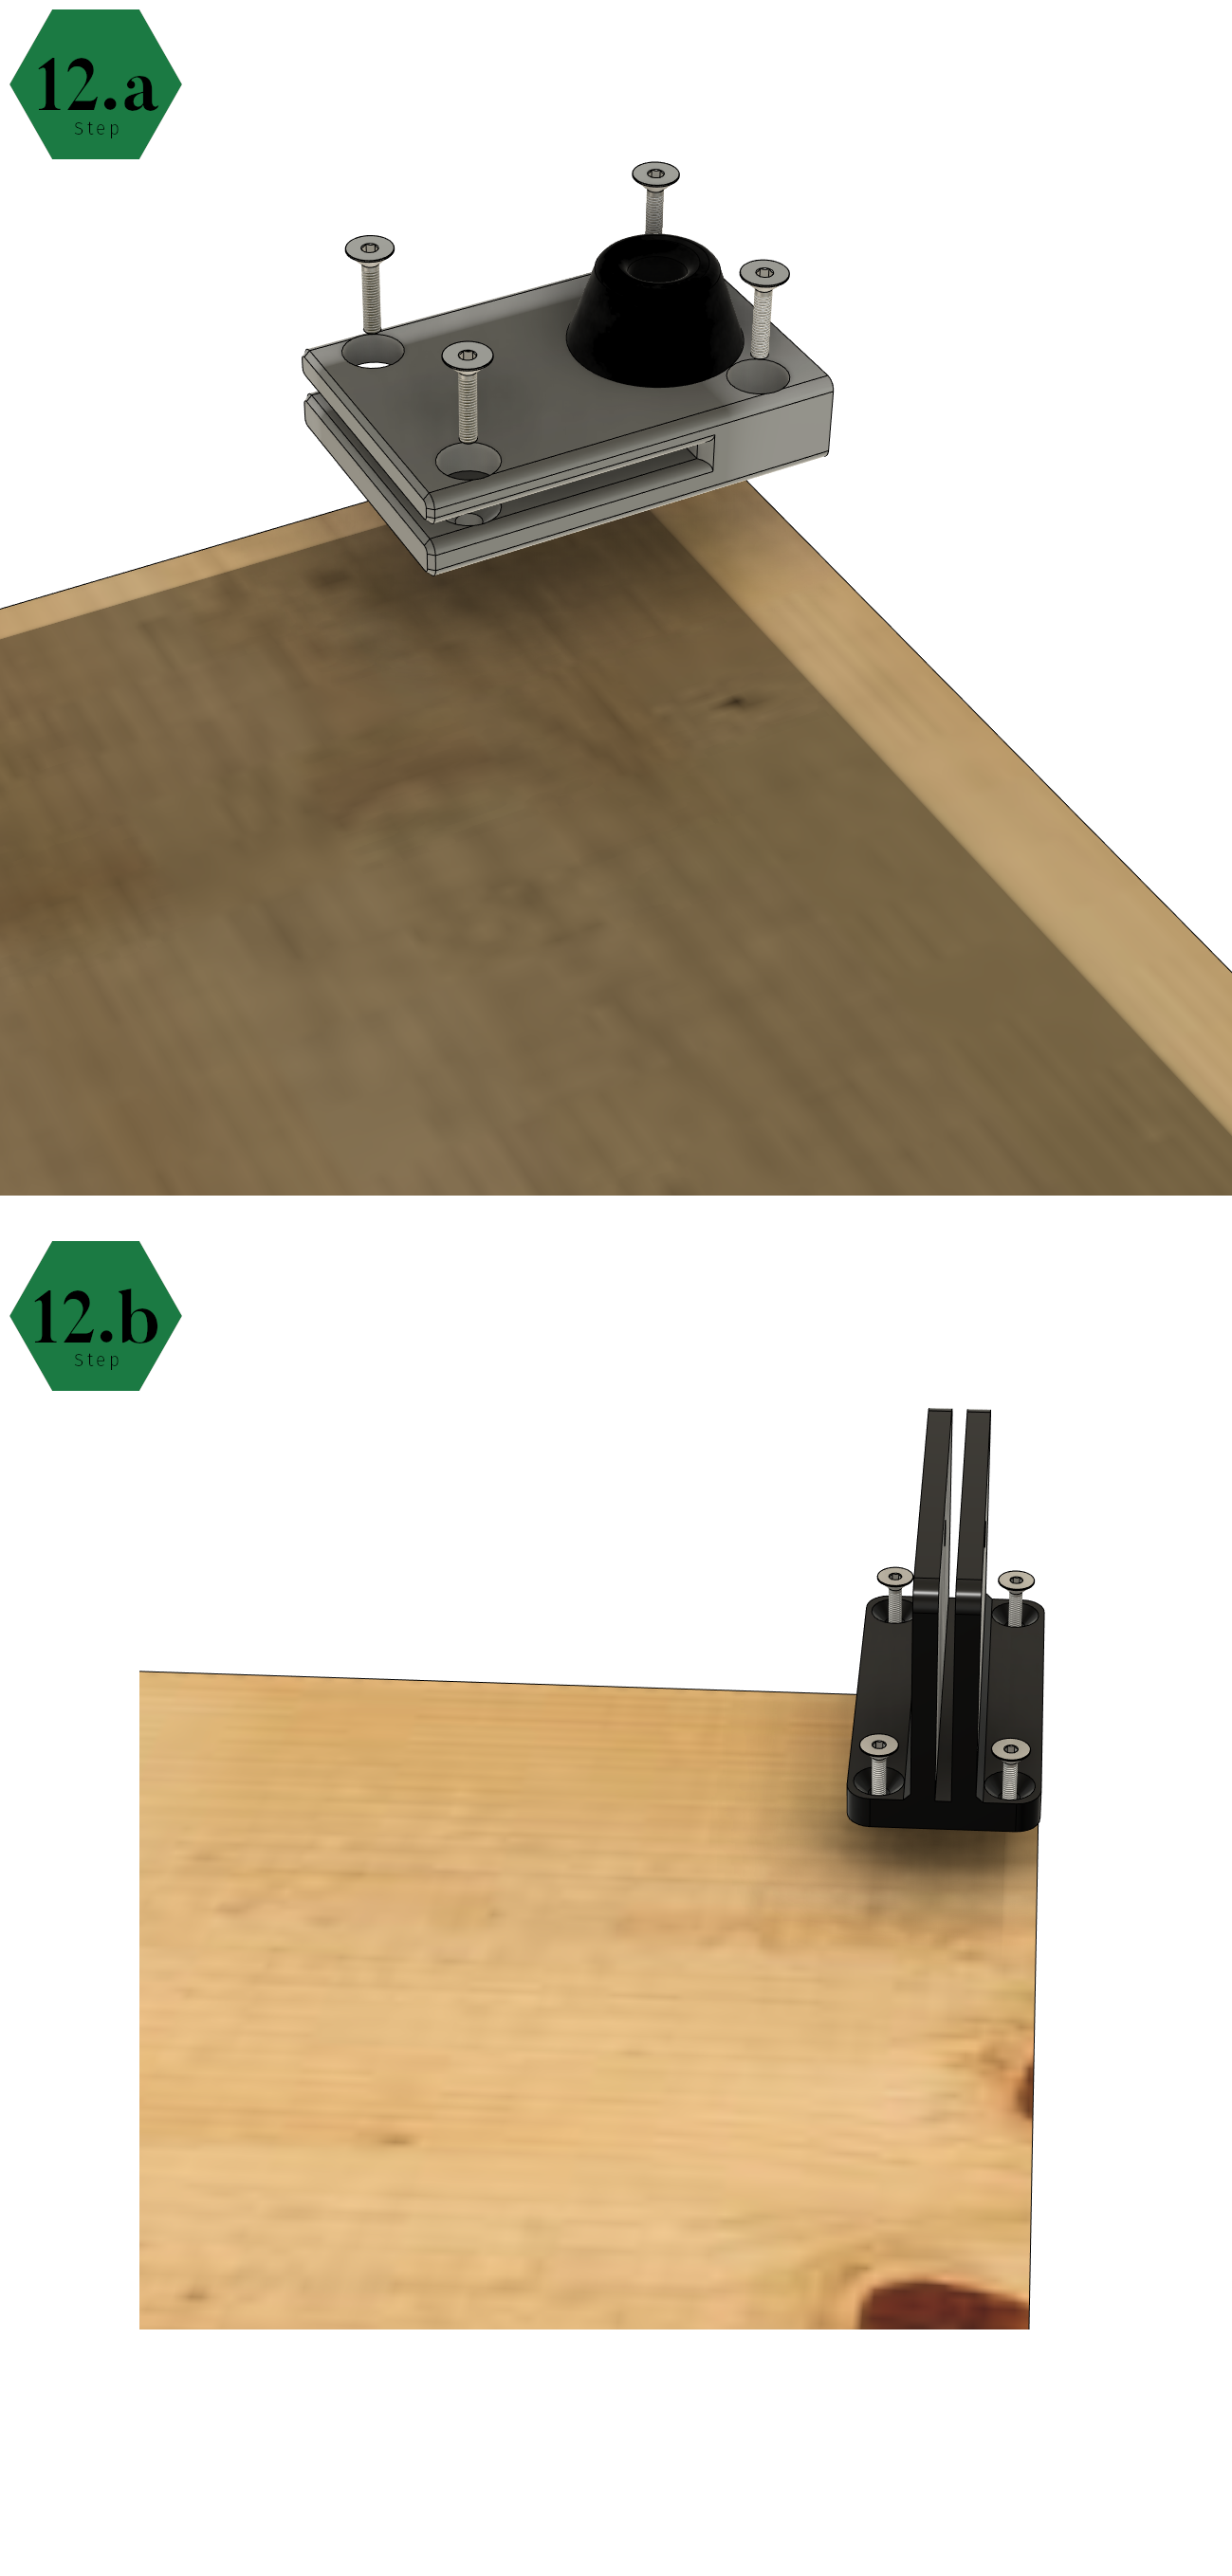
\includegraphics{images/Assembly9.png}%
{\captionof{figure}{Step 12 of the Open3DScanner assembly}}
\clearpage%

% STEP 13
\sideTabularx[Required parts for step 13]{%
	\rowcolors{2}{tableLineTwo}{tableLineOne}% specify rowcolors in tabularx style
	\begin{tabularx} {\marginparwidth} {>{\rowmac \hsize=1.5\hsize}X>{\rowmac \hsize=0.5\hsize}X<{\clearrow}}%
		\tabularxHeader%
		Part & Quantity\\%
		Housing-Main & 1\\%
		\SI{5.5}{\milli\meter}$\times$\SI{2.1}{\milli\meter} Female DC Power Jack Panel Mount (L722AS) & 1\\%
		\SI{5/8}{''} Rubber Seal Ring & 1\\%
	\end{tabularx}%
}%

\marginInfo*[Instructions]{Press the rubber seal into the opening provided in the back of the housing. Mount the power jack in the opening on the left side of the case.}%

\marginTips*[Tip]{If your power jack does not have the accessories for mounting, you will need a M8 nut and a \SI{1}{\milli\meter} washer with \SI{8}{\milli\meter} diameter in addition. Pliers simplify the tightening of the nut. In order to simplify the wiring, it makes sense to attach the power cable to the jack first.}%

\marginCritical*[Warning]{Make sure that the power jack is aligned as shown in the illustration, otherwise the PCB may not fit into the case anymore.}%

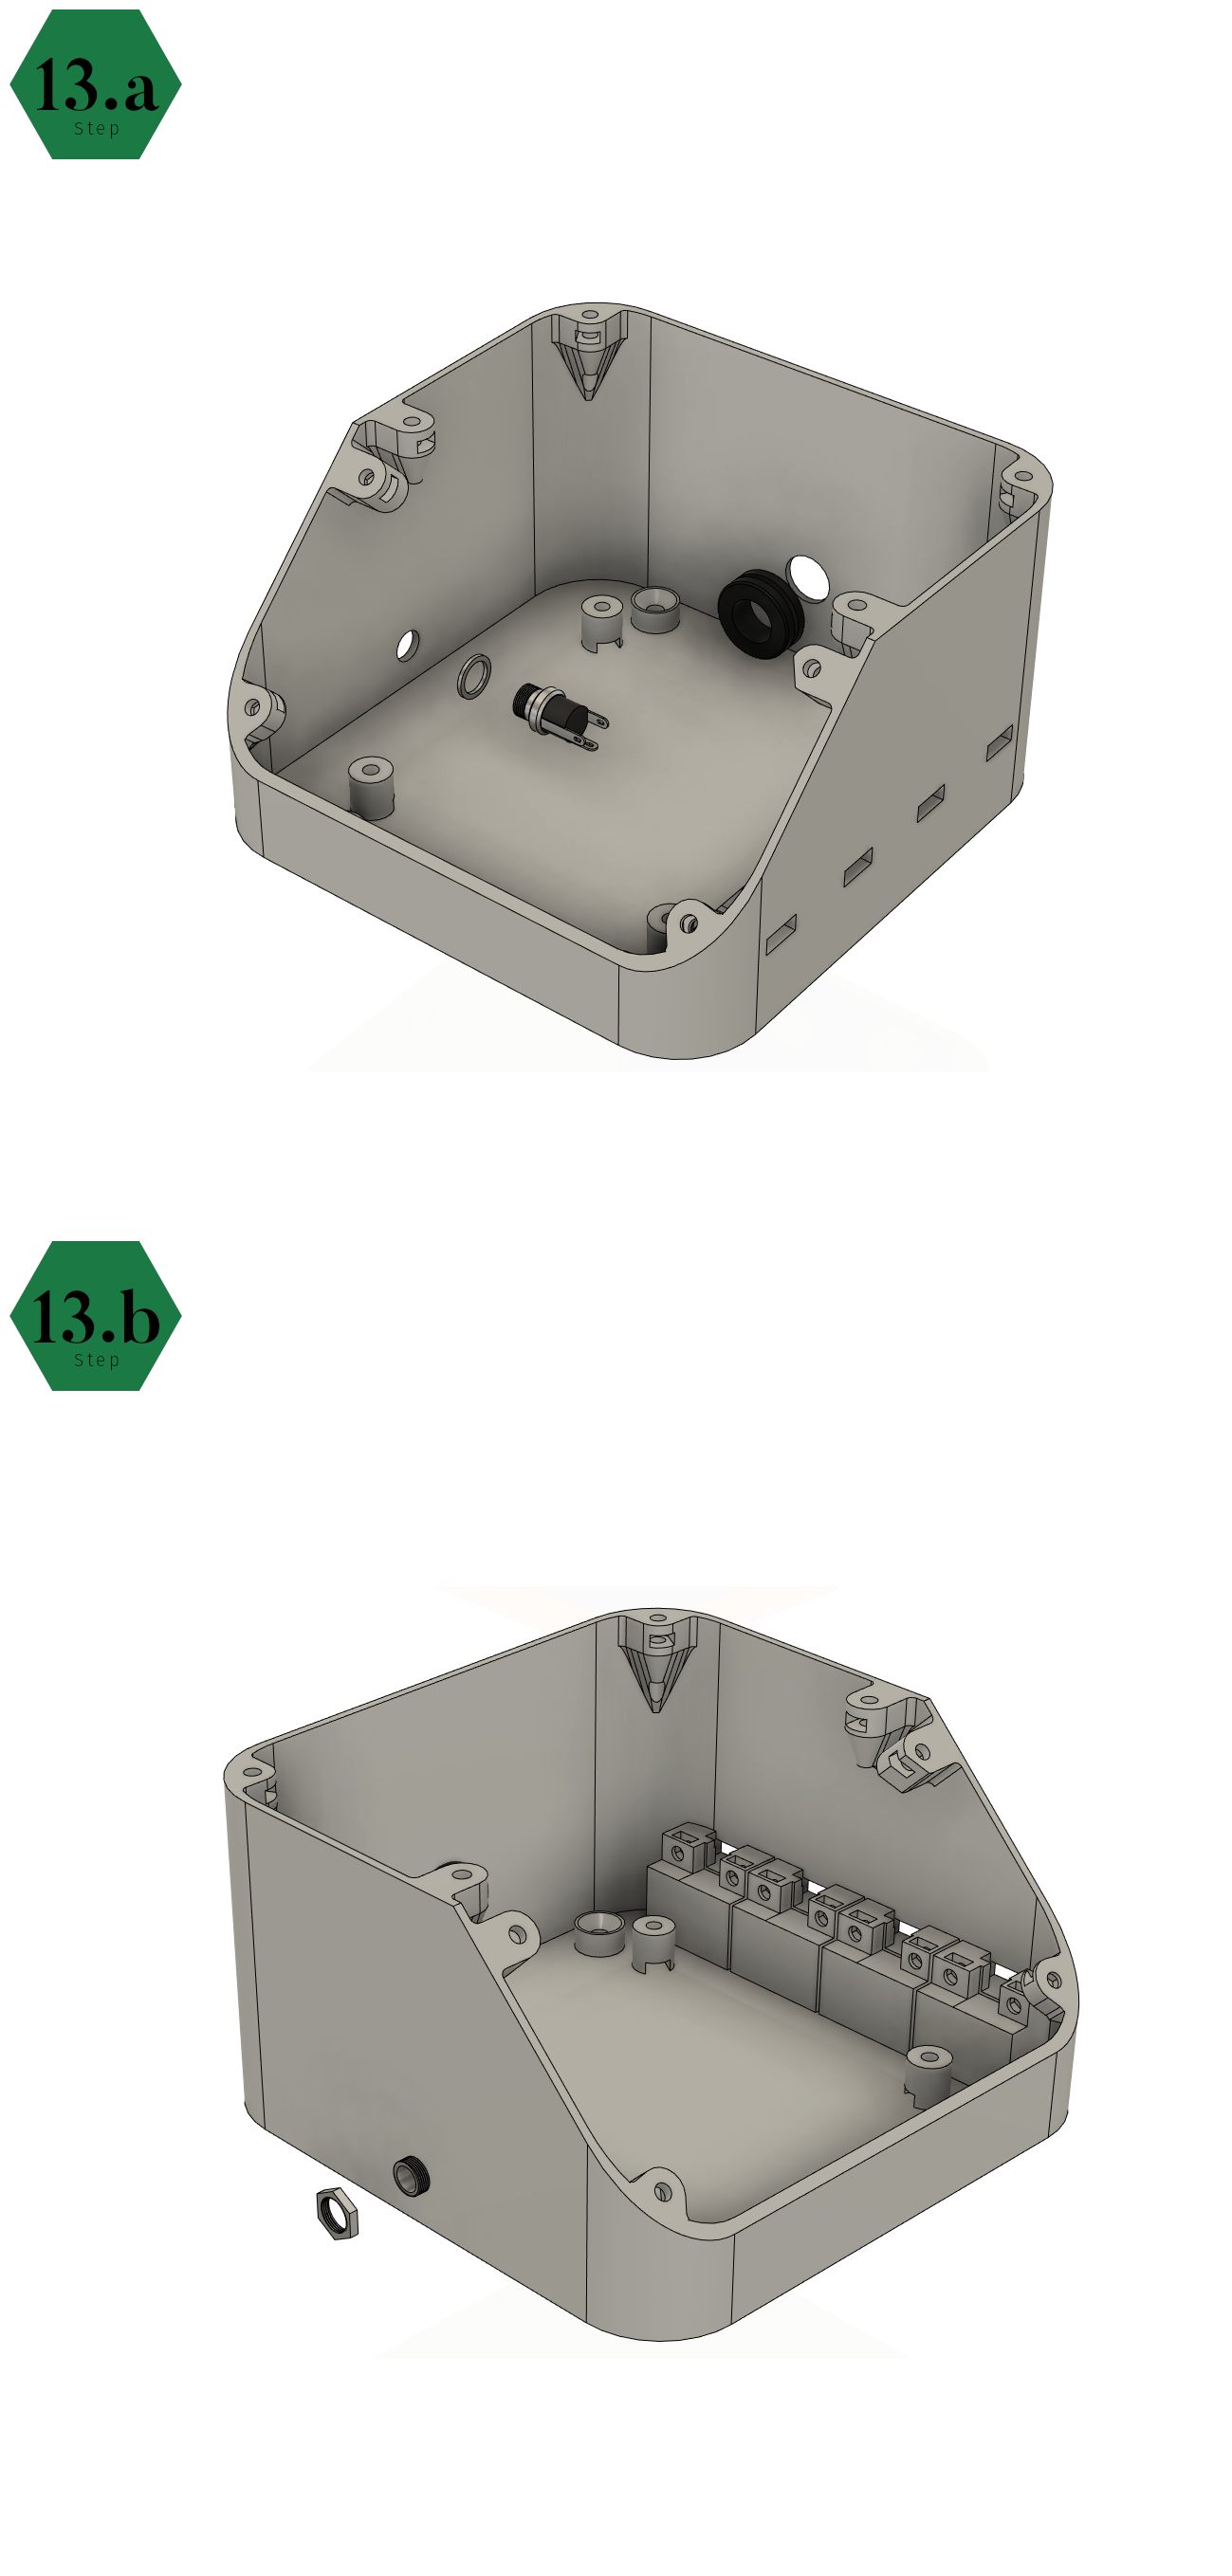
\includegraphics{images/Assembly10.png}%
{\captionof{figure}{Step 13 of the Open3DScanner assembly}}
\clearpage%

% STEP 14
\sideTabularx[Required parts for step 14]{%
	\rowcolors{2}{tableLineTwo}{tableLineOne}% specify rowcolors in tabularx style
	\begin{tabularx} {\marginparwidth} {>{\rowmac \hsize=1.5\hsize}X>{\rowmac \hsize=0.5\hsize}X<{\clearrow}}%
		\tabularxHeader%
		Part & Quantity\\%
		Molex crimp housing --- Micro-Fit - 1x2-pin, male (430200201) & 4\\%
		M3 Nut & 8\\%
	\end{tabularx}%
}%

\marginInfo*[Instructions]{Mount the Micro-Fit connectors. Make sure that the mounting hook points to the rear of the housing. The connectors are first pressed against the housing wall and pushed into the recess. Then they are pushed out a little bit so that they are flush with the outside of the housing. Slide the nuts into the openings.  Two nuts are required for each connector.}%

\marginTips*[Tip]{Before mounting the Micro-Fit connectors, connect the cables to them.}%

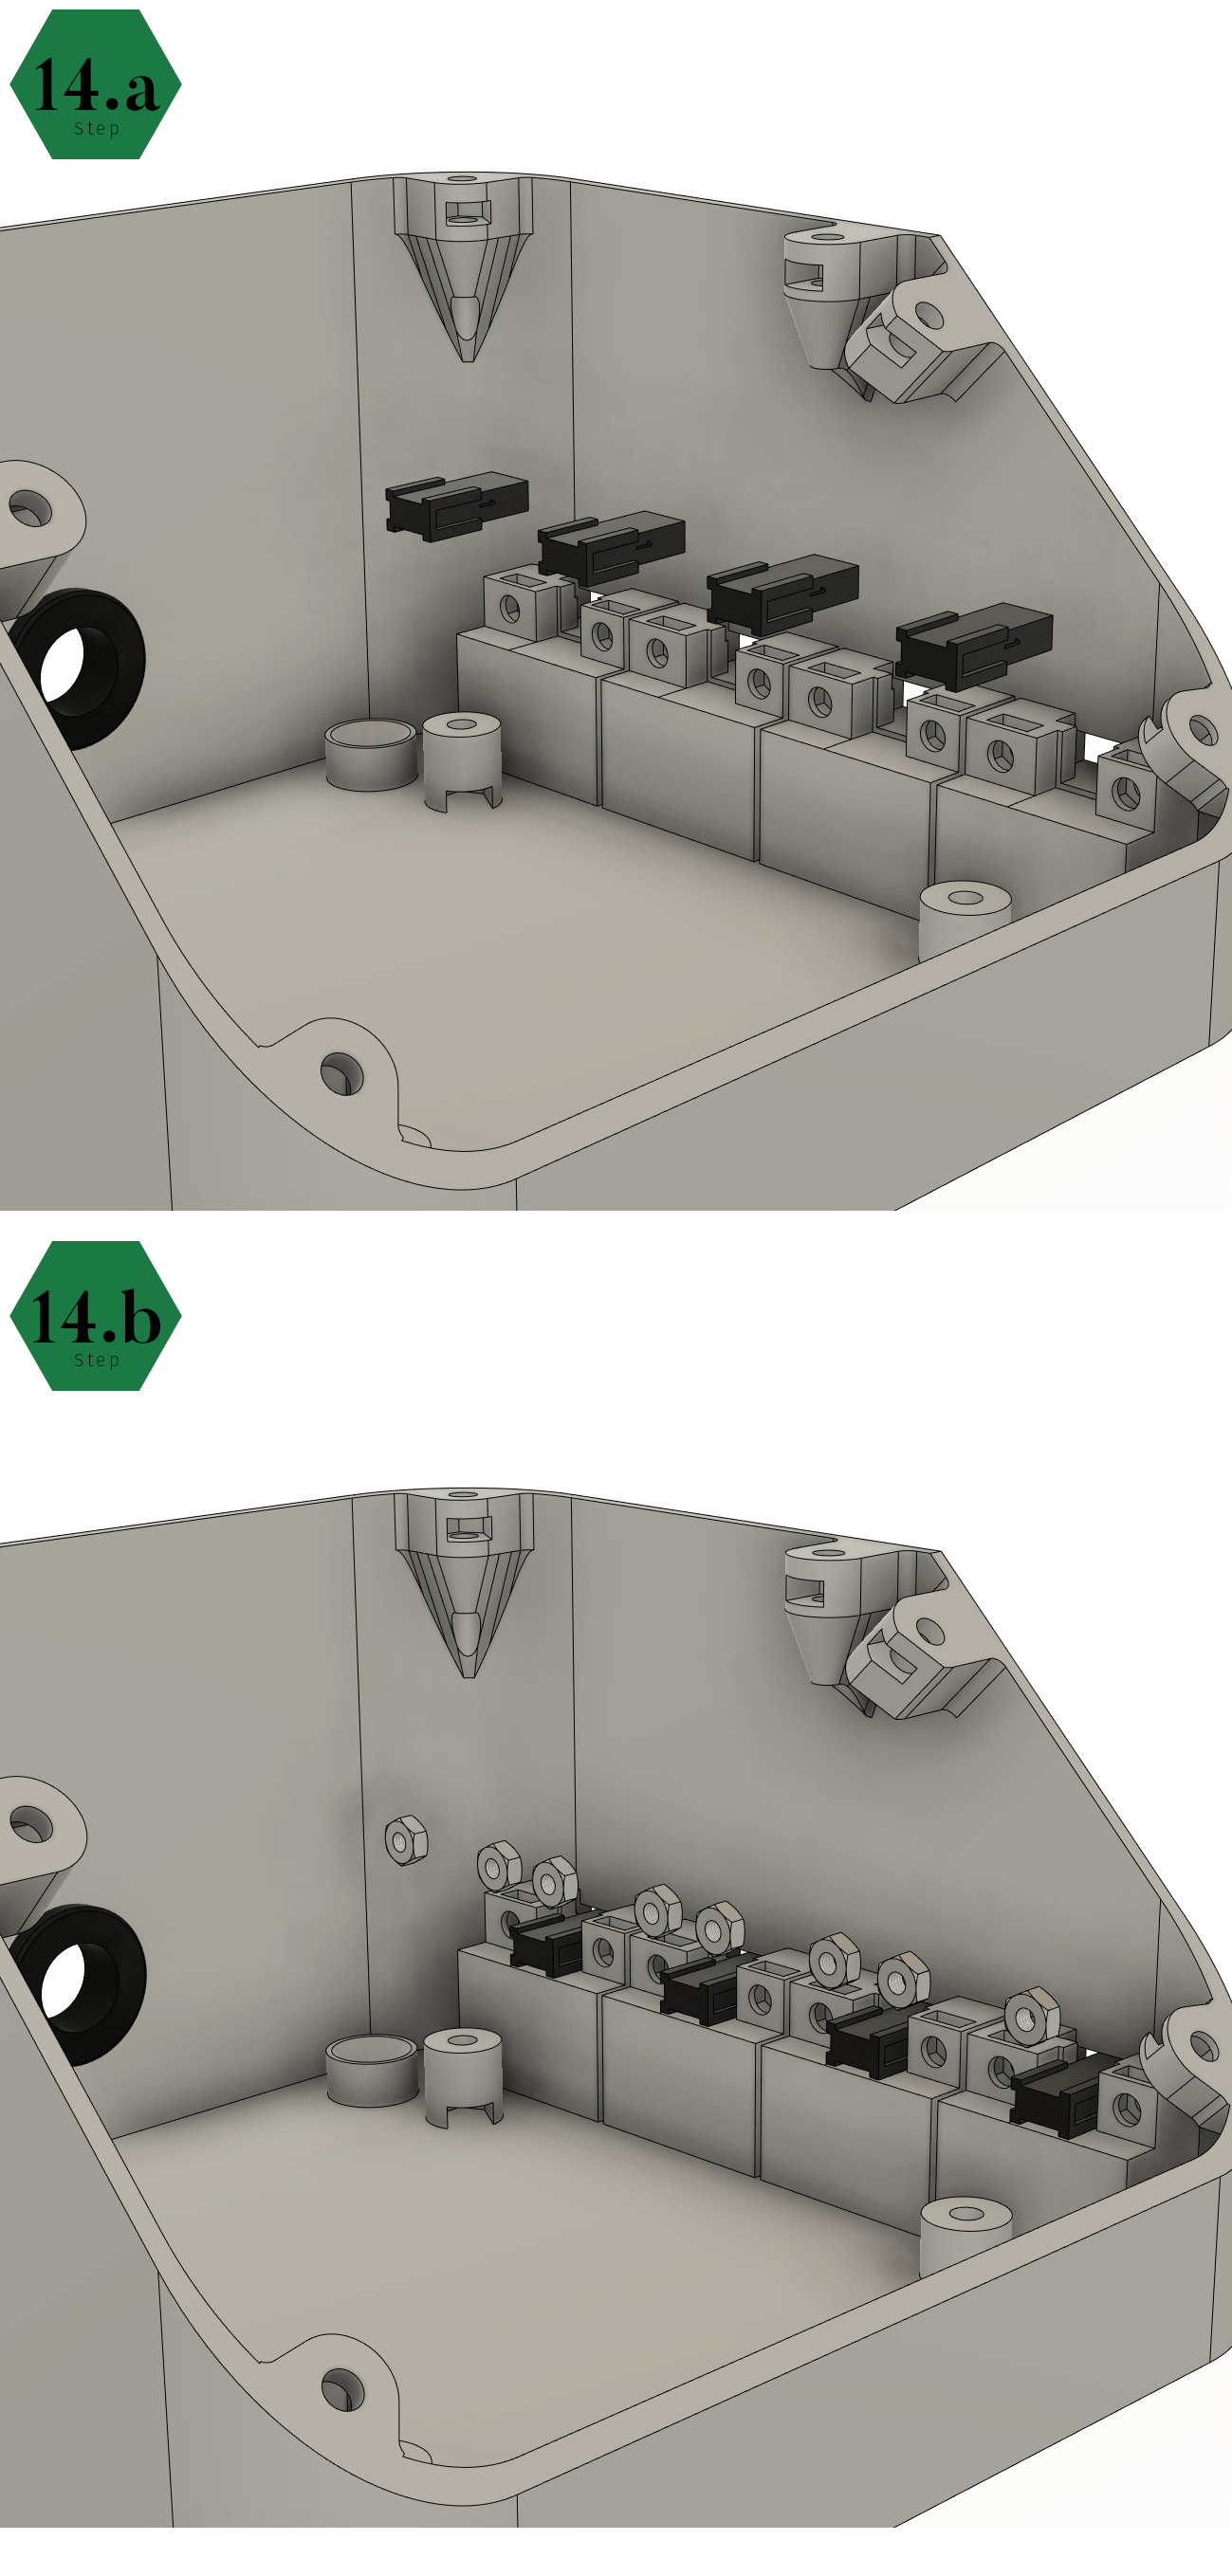
\includegraphics{images/Assembly11.png}%
{\captionof{figure}{Step 14 of the Open3DScanner assembly}}
\clearpage%

% STEP 15 & 16
\sideTabularx[Required parts for step 15]{%
	\rowcolors{2}{tableLineTwo}{tableLineOne}% specify rowcolors in tabularx style
	\begin{tabularx} {\marginparwidth} {>{\rowmac \hsize=1.5\hsize}X>{\rowmac \hsize=0.5\hsize}X<{\clearrow}}%
		\tabularxHeader%
		Part & Quantity\\%
		Micro-Fit-Holder-P1 & 4\\%
		Micro-Fit-Holder-P2 & 4\\%
		M3$\times$10 & 8\\%
	\end{tabularx}%
}%

\marginInfo*[Instructions]{Use one Micro-Fit-Holder-P1, one Micro-Fit-Holder-P1, and two screws to secure each Micro-Fit connectors.}%

\sideTabularx[Required parts for step 16]{%
	\vspace{4.5cm}%
	\rowcolors{2}{tableLineTwo}{tableLineOne}% specify rowcolors in tabularx style
	\begin{tabularx} {\marginparwidth} {>{\rowmac \hsize=1.5\hsize}X>{\rowmac \hsize=0.5\hsize}X<{\clearrow}}%
		\tabularxHeader%
		Part & Quantity\\%
		M3 Nut & 8\\%
	\end{tabularx}%
}%

\marginInfo*[Instructions]{Slide a nut into each opening along the top edge of the housing.}%

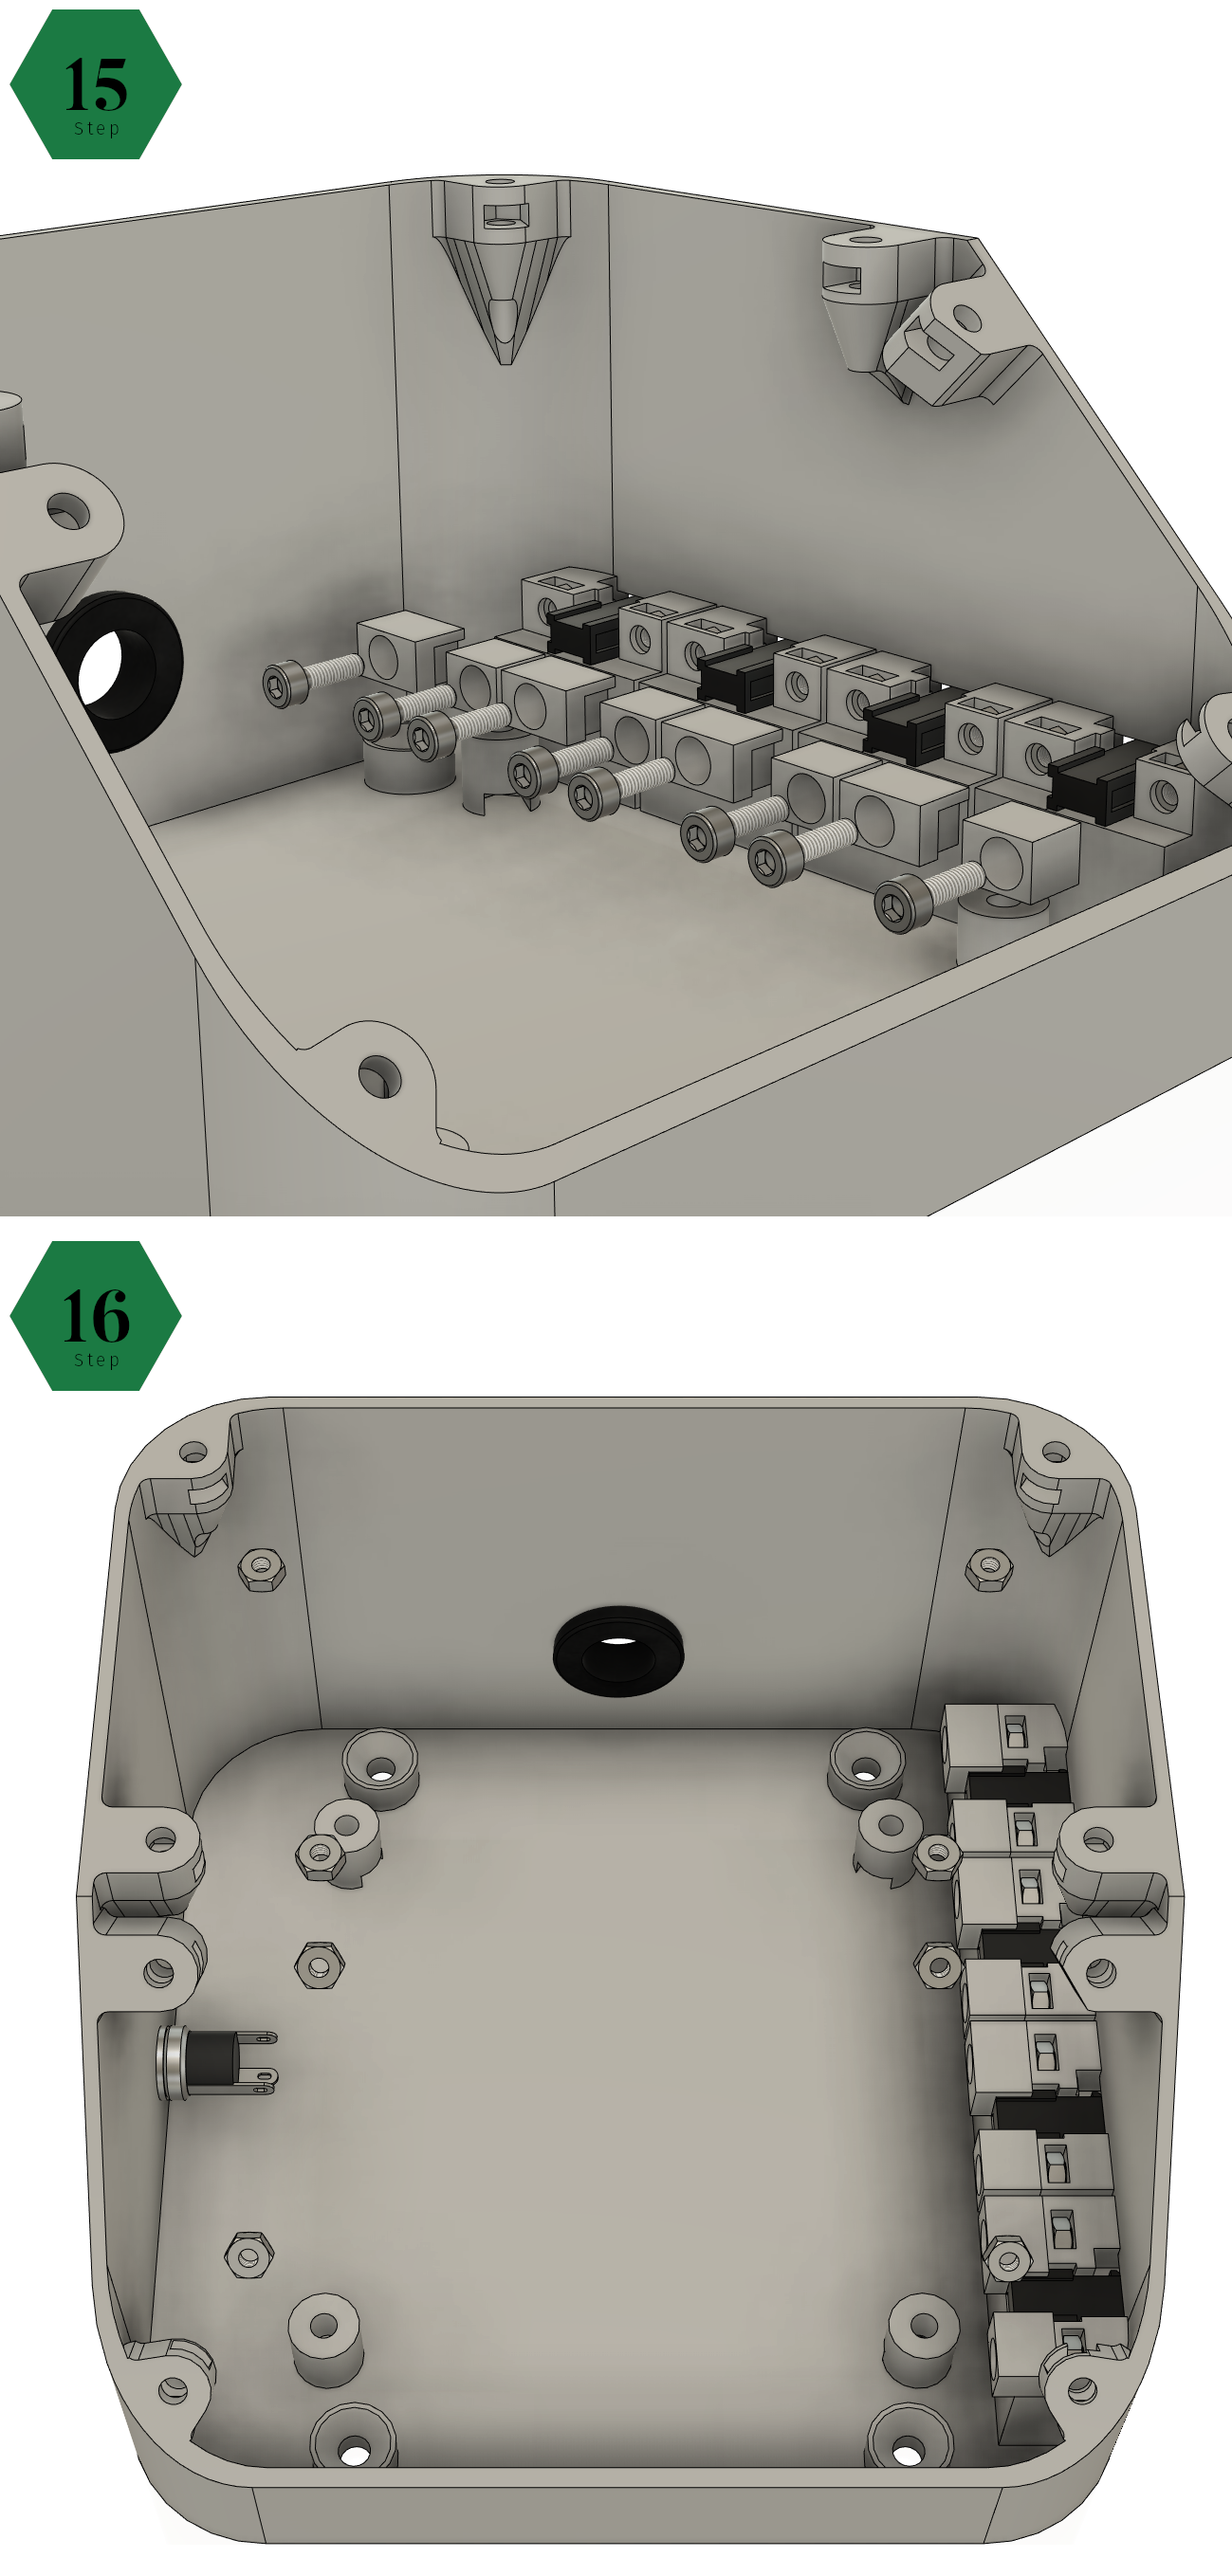
\includegraphics{images/Assembly12.png}%
{\captionof{figure}{Step 15 \& 16 of the Open3DScanner assembly}}
\clearpage%

% STEP 17
\sideTabularx[Required parts for step 17]{%
	\rowcolors{2}{tableLineTwo}{tableLineOne}% specify rowcolors in tabularx style
	\begin{tabularx} {\marginparwidth} {>{\rowmac \hsize=1.5\hsize}X>{\rowmac \hsize=0.5\hsize}X<{\clearrow}}%
		\tabularxHeader%
		Part & Quantity\\%
		PCB & 1\\%
		M3 Nut & 4\\%
		M3$\times$12 & 4\\%
	\end{tabularx}%
}%

\marginInfo*[Instructions]{Slide one nut each into the PCB stand at the bottom of the housing. Then screw the PCB into the housing.}%

\marginTips*[Tip]{The cable from the power jack can be routed below the PCB. This is much easier if it is done before the PCB is screwed down.}%

\marginCheck*[Check]{Make sure that you align the PCB as shown in the figure, otherwise the wiring may become difficult and the specified cable lengths will no longer fit.}%

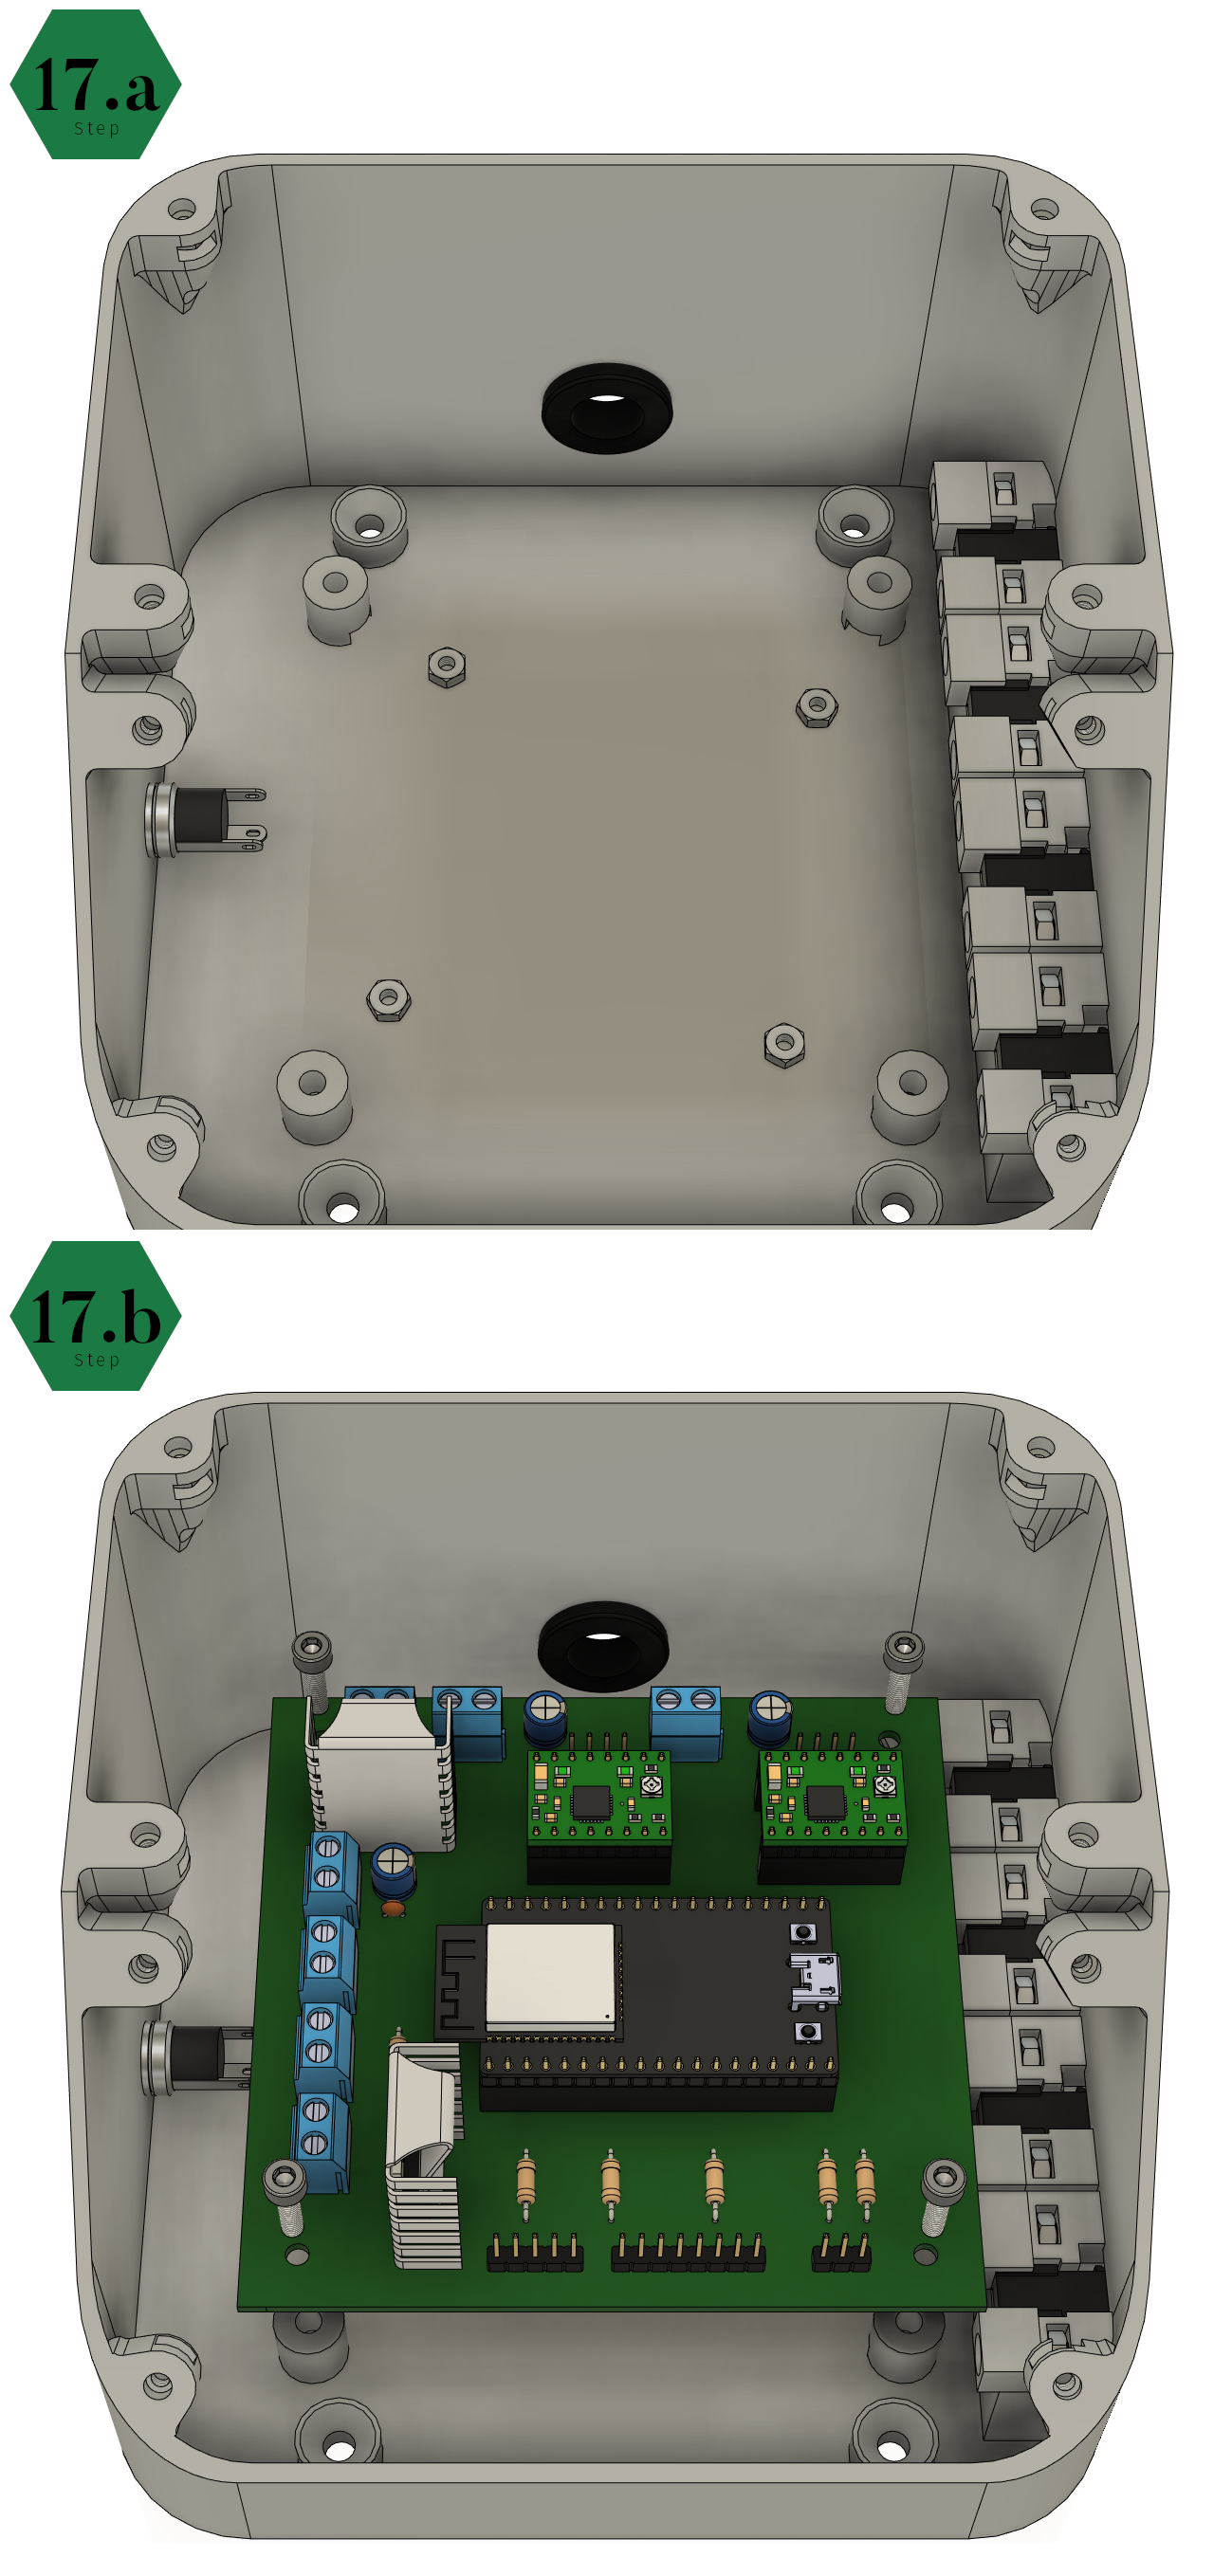
\includegraphics{images/Assembly13.png}%
{\captionof{figure}{Step 17 of the Open3DScanner assembly}}
\clearpage%

% STEP 18 & 19
\sideTabularx[Required parts for step 18]{%
	\rowcolors{2}{tableLineTwo}{tableLineOne}% specify rowcolors in tabularx style
	\begin{tabularx} {\marginparwidth} {>{\rowmac \hsize=1.5\hsize}X>{\rowmac \hsize=0.5\hsize}X<{\clearrow}}%
		\tabularxHeader%
		Part & Quantity\\%
		4.0$\times$16 Countersunk Wood Screwt & 4\\%
	\end{tabularx}%
}%

\marginInfo*[Instructions]{Screw the housing onto the wooden base plate.}%

\marginTips*[Tip]{For the exact alignment on the base plate, there is a detailed illustration at the end of the assembly instructions.}%

\sideTabularx[Required parts for step 19]{%
	\vspace{1.80cm}%
	\rowcolors{2}{tableLineTwo}{tableLineOne}% specify rowcolors in tabularx style
	\begin{tabularx} {\marginparwidth} {>{\rowmac \hsize=1.5\hsize}X>{\rowmac \hsize=0.5\hsize}X<{\clearrow}}%
		\tabularxHeader%
		Part & Quantity\\%
		STEC12E08 Rotary Encoder & 1\\%
		\SI{5}{\milli\meter} 3-Pin Bi-Color LED & 1\\%
		Nokia 5110 Display & 1\\%
		LCD-Holder & 4\\%
		LED-Holder & 1\\%
		Encoder-Holder & 1\\%
		Housing-Front & 1\\%
		M3$\times$12 & 2\\%
		M3$\times$6 & 2\\%
		M3 Nut & 8\\%
	\end{tabularx}%
}%

\marginInfo*[Instructions]{Glue the nuts for the LED and the encoder with superglue into the front panel of the housing. Press the remaining nuts into the LCD-holder. Insert the LED, encoder, and LCD into the openings provided in the front panel. Screw the LED and encoder to the front panel. Use LED-Holder and Encoder-Holder for this.}%

\marginTips*[Tip]{Depending on the manufacturer of the LCD, it may be necessary to cut a piece out of the back of the front panel, otherwise the solder points will prevent the display from sitting flush in the panel.}%

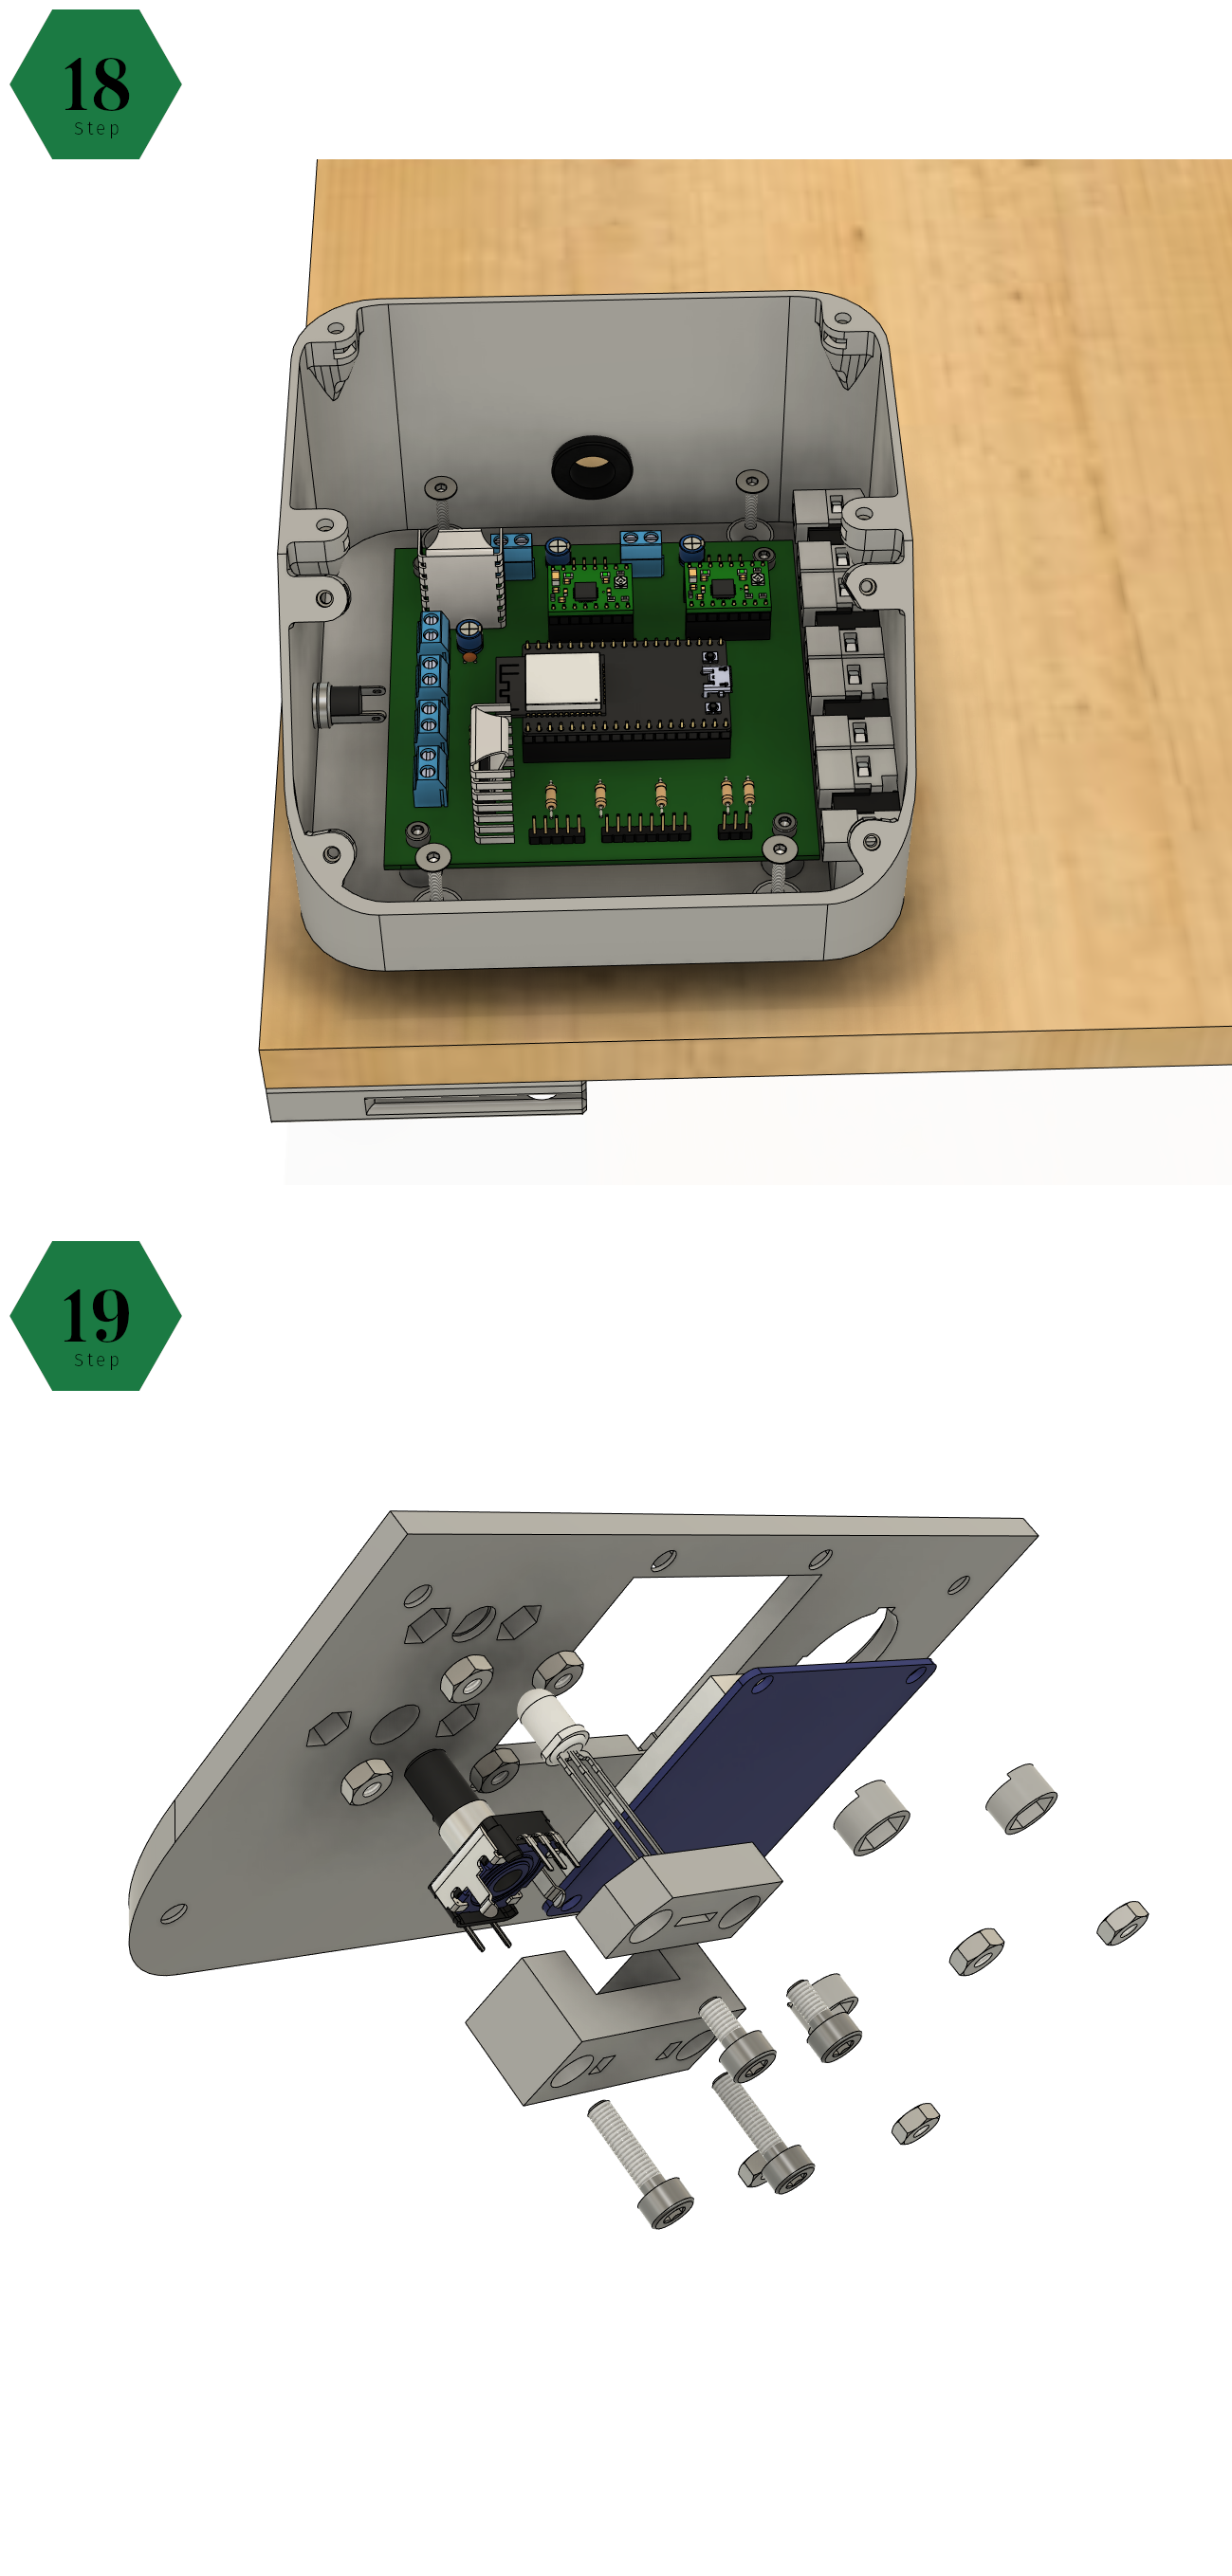
\includegraphics{images/Assembly14.png}%
{\captionof{figure}{Step 18 \& 19 of the Open3DScanner assembly}}
\clearpage%

% STEP 20 & 21
\sideTabularx[Required parts for step 20]{%
	\rowcolors{2}{tableLineTwo}{tableLineOne}% specify rowcolors in tabularx style
	\begin{tabularx} {\marginparwidth} {>{\rowmac \hsize=1.5\hsize}X>{\rowmac \hsize=0.5\hsize}X<{\clearrow}}%
		\tabularxHeader%
		Part & Quantity\\%
		Housing-Knob & 1\\%
		Round \SI{20}{\milli\meter} SPST Rocker Switch (R13 112) & 1\\%
		M3$\times$10  & 4\\%
	\end{tabularx}%
}%

\marginInfo*[Instructions]{Press the rocker switch into the recess of the front panel. Screw the display tight and pay attention to the orientation of the LCD-Holder. Press the Housing-Knob onto the shaft of the encoder.}%

\marginTips*[Tip]{Do not press the Housing-Knob too firmly on the shaft, otherwise the glued nuts will come loose.}%


\sideTabularx[Required parts for step 21]{%
	\vspace{0.80cm}%
	\rowcolors{2}{tableLineTwo}{tableLineOne}% specify rowcolors in tabularx style
	\begin{tabularx} {\marginparwidth} {>{\rowmac \hsize=1.5\hsize}X>{\rowmac \hsize=0.5\hsize}X<{\clearrow}}%
		\tabularxHeader%
		Part & Quantity\\%
		Housing-Top  & 1\\%
		M3$\times$10  & 8\\%
	\end{tabularx}%
}%

\marginInfo*[Instructions]{Screw the Housing-Top and the assembled Housing-Front to the housing.}%

\marginTips*[Tip]{Before you screw the front panel to the housing, all cables should be connected inside the housing and the stepper motors should also be connected to the PCB. Also ensure that you flashed the firmware to the ESP32. I recommend a basic functionality test before closing the housing.}%

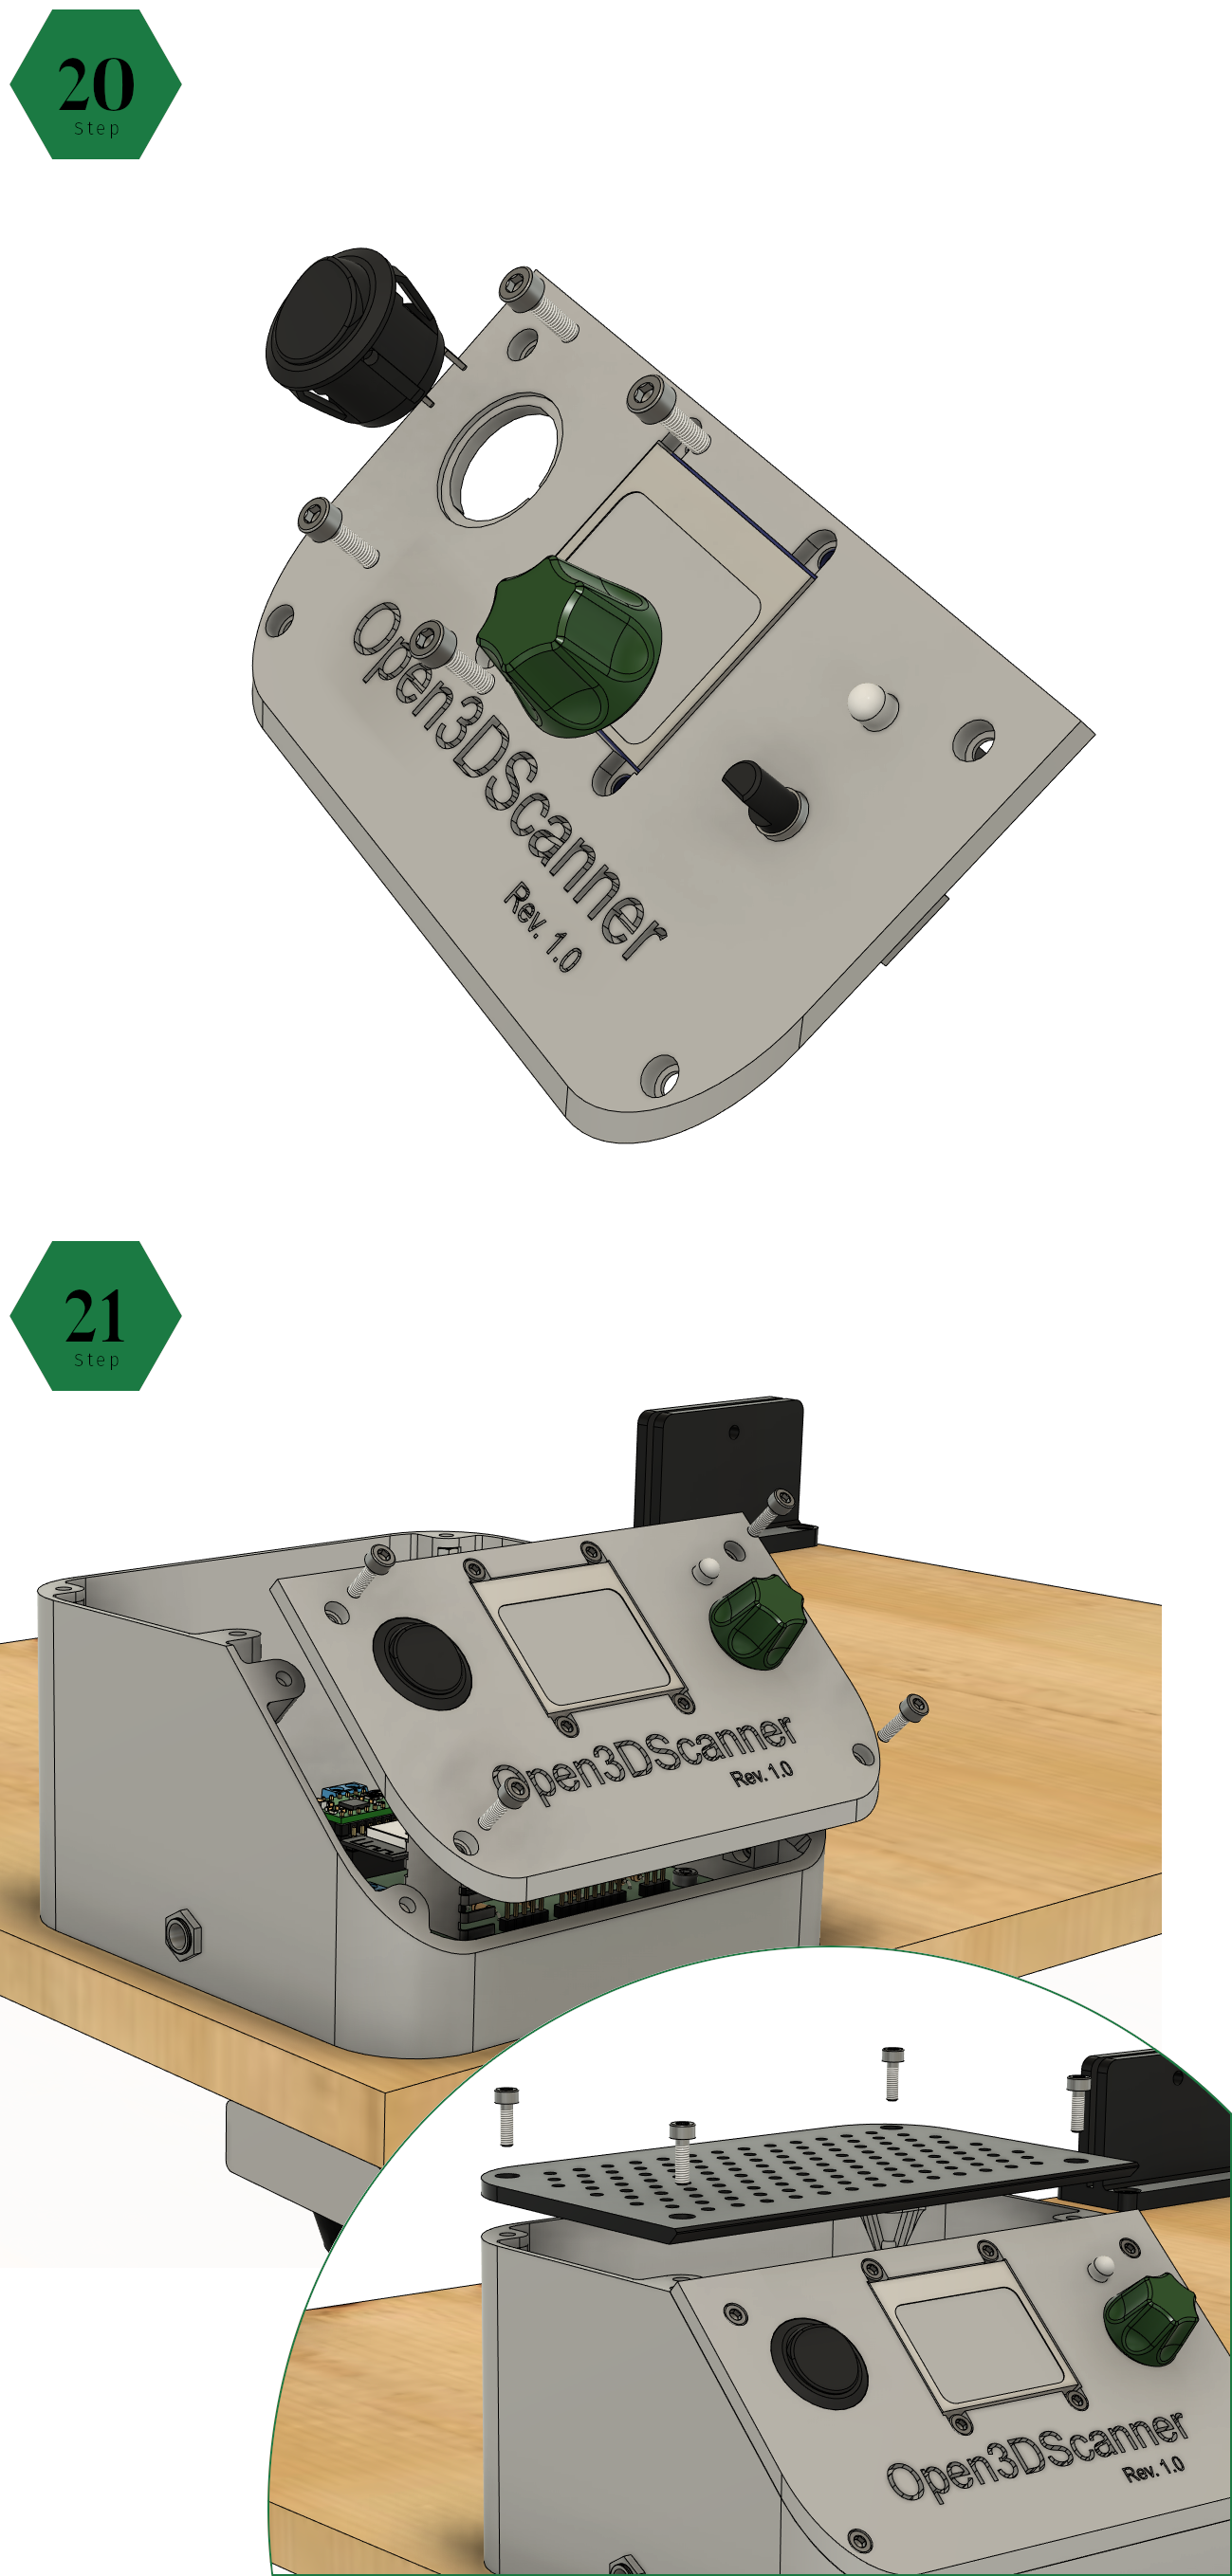
\includegraphics{images/Assembly15.png}%
{\captionof{figure}{Step 20 \& 21 of the Open3DScanner assembly}}
\clearpage%

% STEP 22 & 23
\sideTabularx[Required parts for step 22]{%
	\rowcolors{2}{tableLineTwo}{tableLineOne}% specify rowcolors in tabularx style
	\begin{tabularx} {\marginparwidth} {>{\rowmac \hsize=1.5\hsize}X>{\rowmac \hsize=0.5\hsize}X<{\clearrow}}%
		\tabularxHeader%
		Part & Quantity\\%
		4.0$\times$16 Countersunk Wood Screwt & 6\\%
	\end{tabularx}%
}%

\marginInfo*[Instructions]{Screw the assembled scanner onto the base plate.}%

\marginTips*[Tip]{For the exact alignment on the base plate, there is a detailed illustration at the end of the assembly instructions.}%

\sideTabularx[Required parts for step 23]{%
	\vspace{3.30cm}%
	\rowcolors{2}{tableLineTwo}{tableLineOne}% specify rowcolors in tabularx style
	\begin{tabularx} {\marginparwidth} {>{\rowmac \hsize=1.5\hsize}X>{\rowmac \hsize=0.5\hsize}X<{\clearrow}}%
		\tabularxHeader%
		Part & Quantity\\%
		4.0$\times$16 Countersunk Wood Screwt & 6\\%
	\end{tabularx}%
}%

\marginInfo*[Instructions]{Screw the assembled lights onto the base plate.}%

\marginTips*[Tip]{For the exact alignment on the base plate, there is a detailed illustration at the end of the assembly instructions.}%

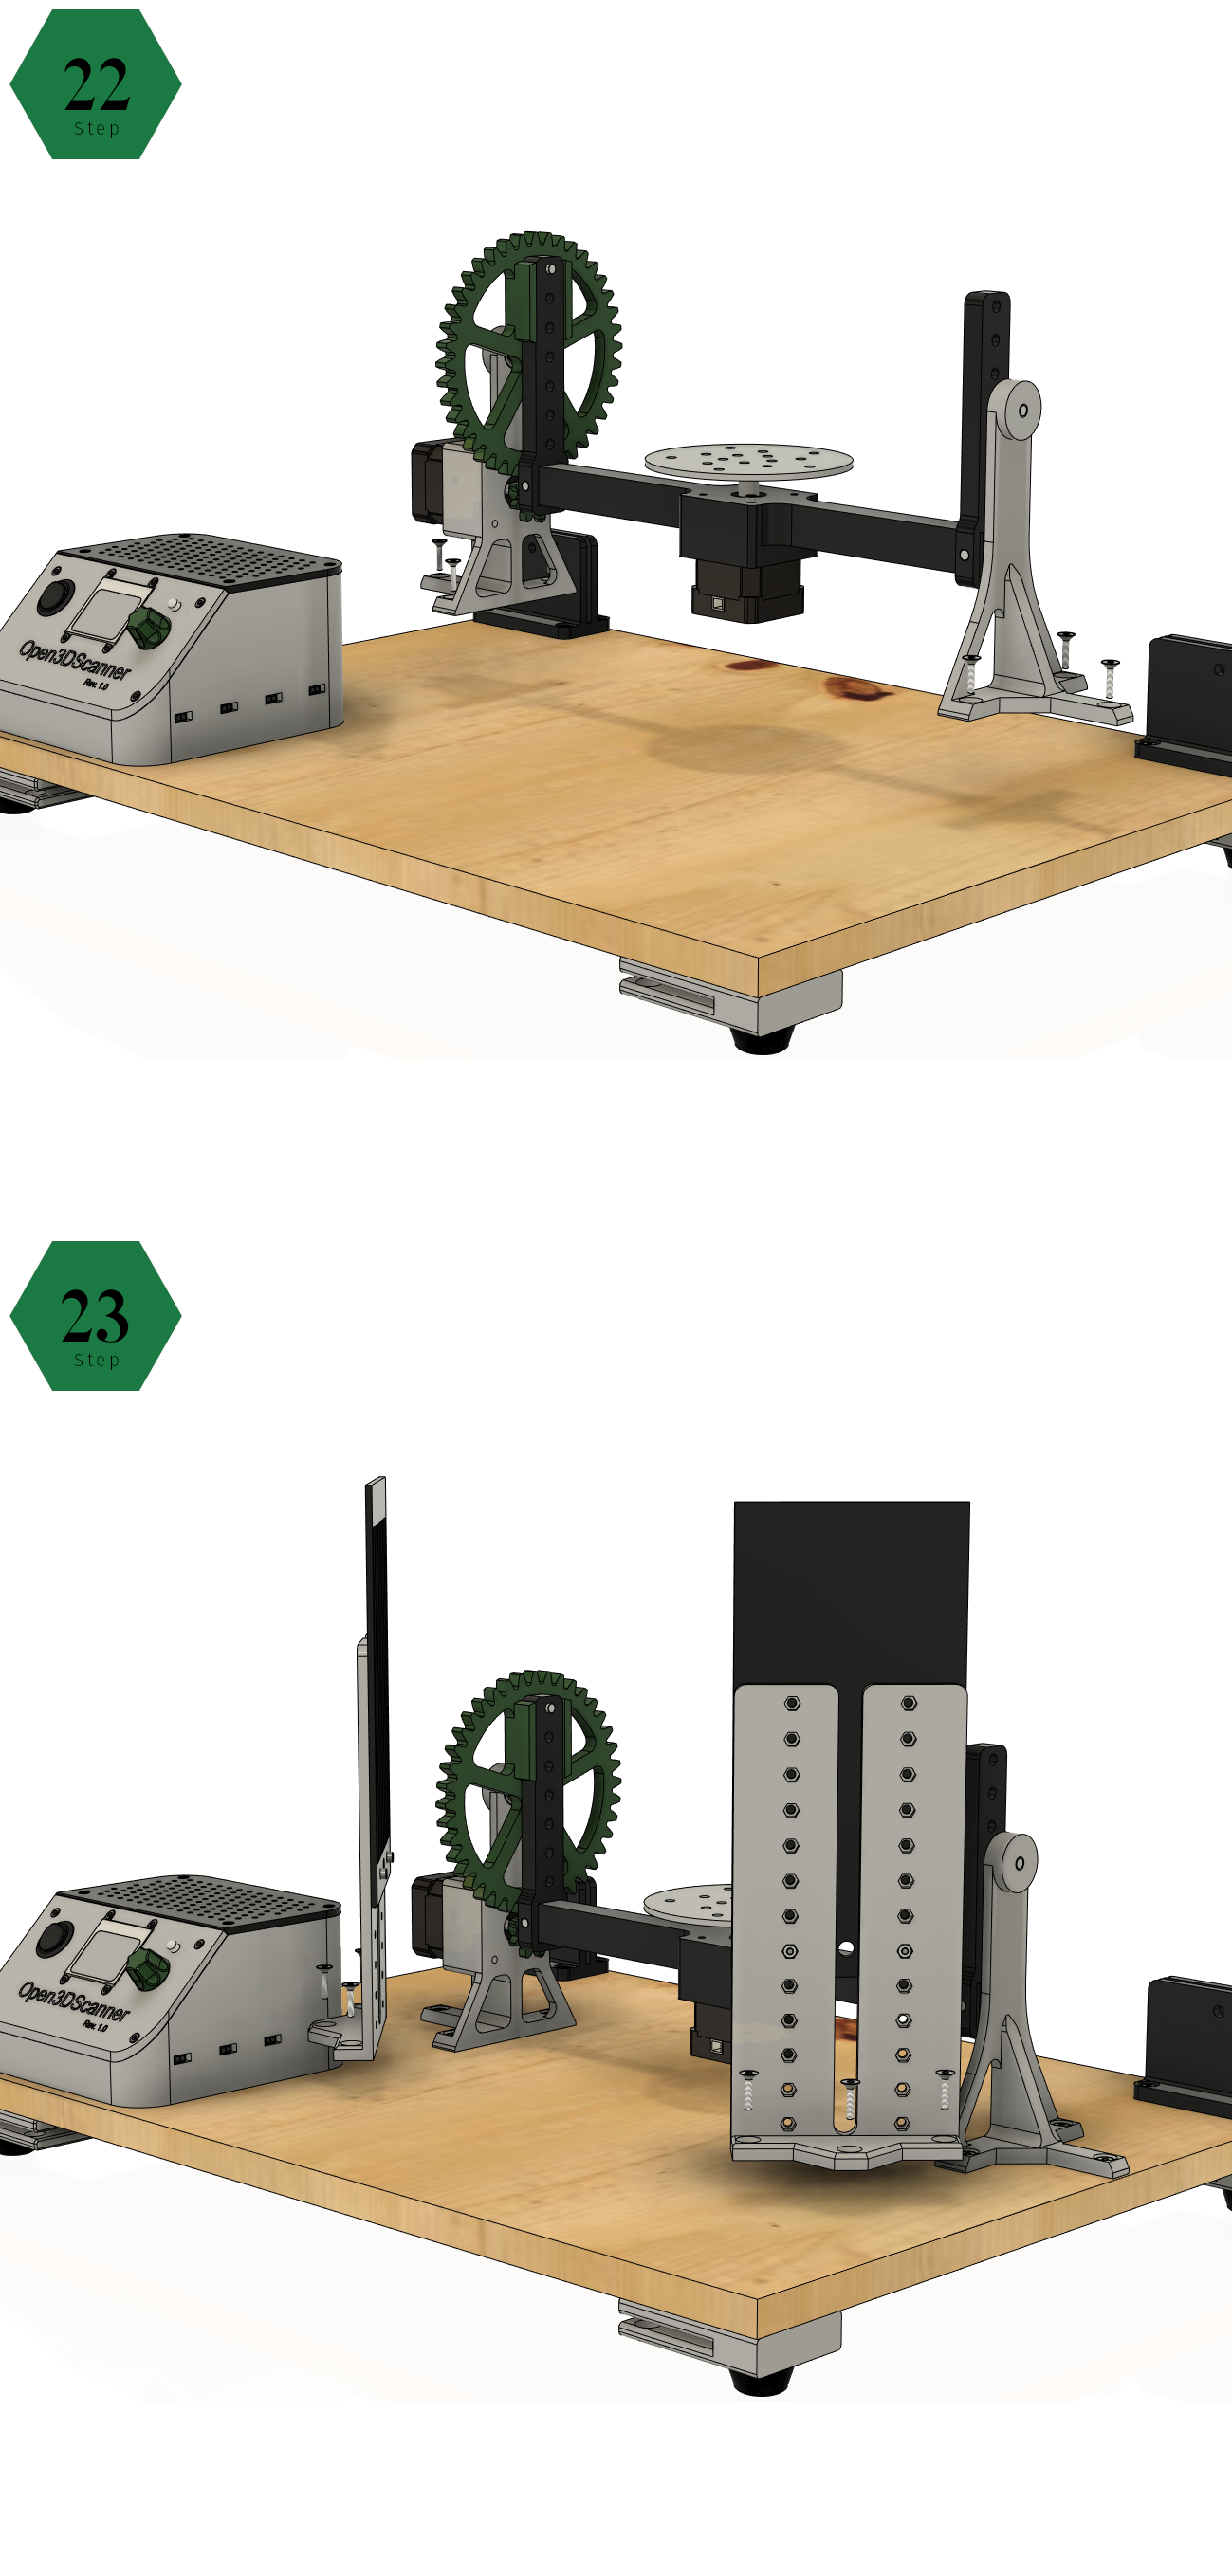
\includegraphics{images/Assembly16.png}%
{\captionof{figure}{Step 22 \& 23 of the Open3DScanner assembly}}
\clearpage%

% STEP 24 & Fin
\sideTabularx[Required parts for step 24]{%
	\rowcolors{2}{tableLineTwo}{tableLineOne}% specify rowcolors in tabularx style
	\begin{tabularx} {\marginparwidth} {>{\rowmac \hsize=1.5\hsize}X>{\rowmac \hsize=0.5\hsize}X<{\clearrow}}%
		\tabularxHeader%
		Part & Quantity\\%
		Cable-Holder & 5\\%
		4.0$\times$16 Countersunk Wood Screwt & 10\\%
	\end{tabularx}%
}%

\marginInfo*[Instructions]{Screw the cable holders onto the base plate.}%

\marginTips*[Tip]{For the exact alignment on the base plate, there is a detailed illustration at the end of the assembly instructions. All cables have to be routed for this step.}%

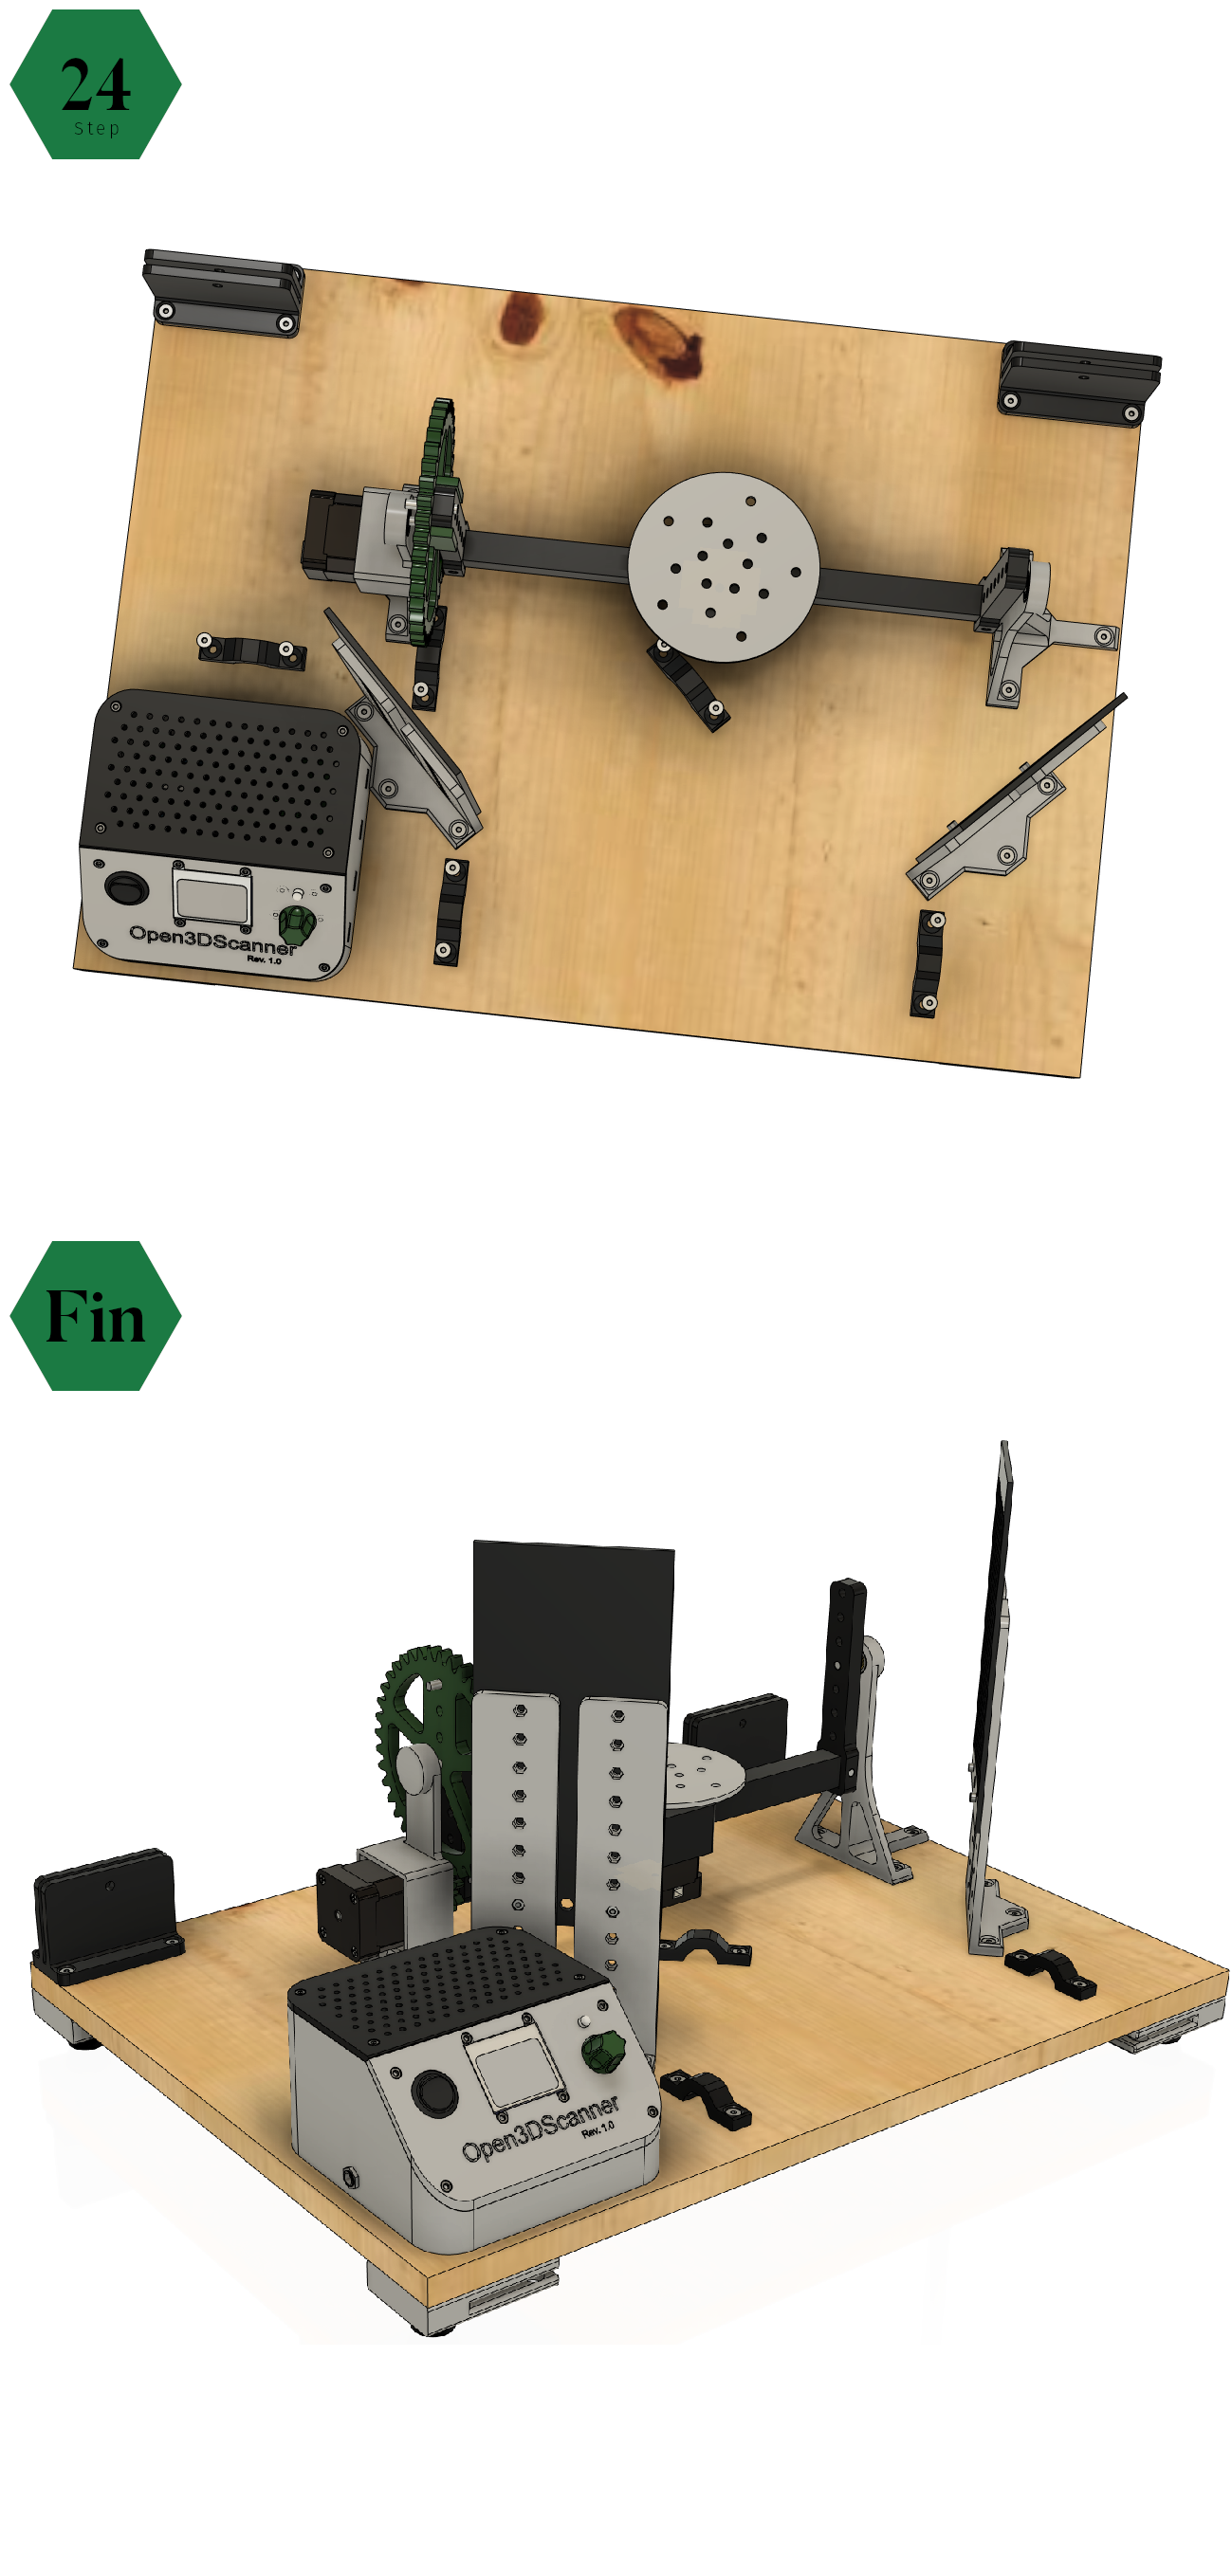
\includegraphics{images/Assembly17.png}%
{\captionof{figure}{Step 24 \& Fin of the Open3DScanner assembly}}
\clearpage%

% ALIGNMENT


\marginTips*[Tip]{This illustration is an aid for aligning the components on the base plate. All values are given in millimeters. For the individual setup, the values can deviate slightly, especially the distance between the two stands of the 3D scanner. This is due to the fact that a certain tolerance is given by the steel bars. Figure B shows the dimensions of the back plate.}%

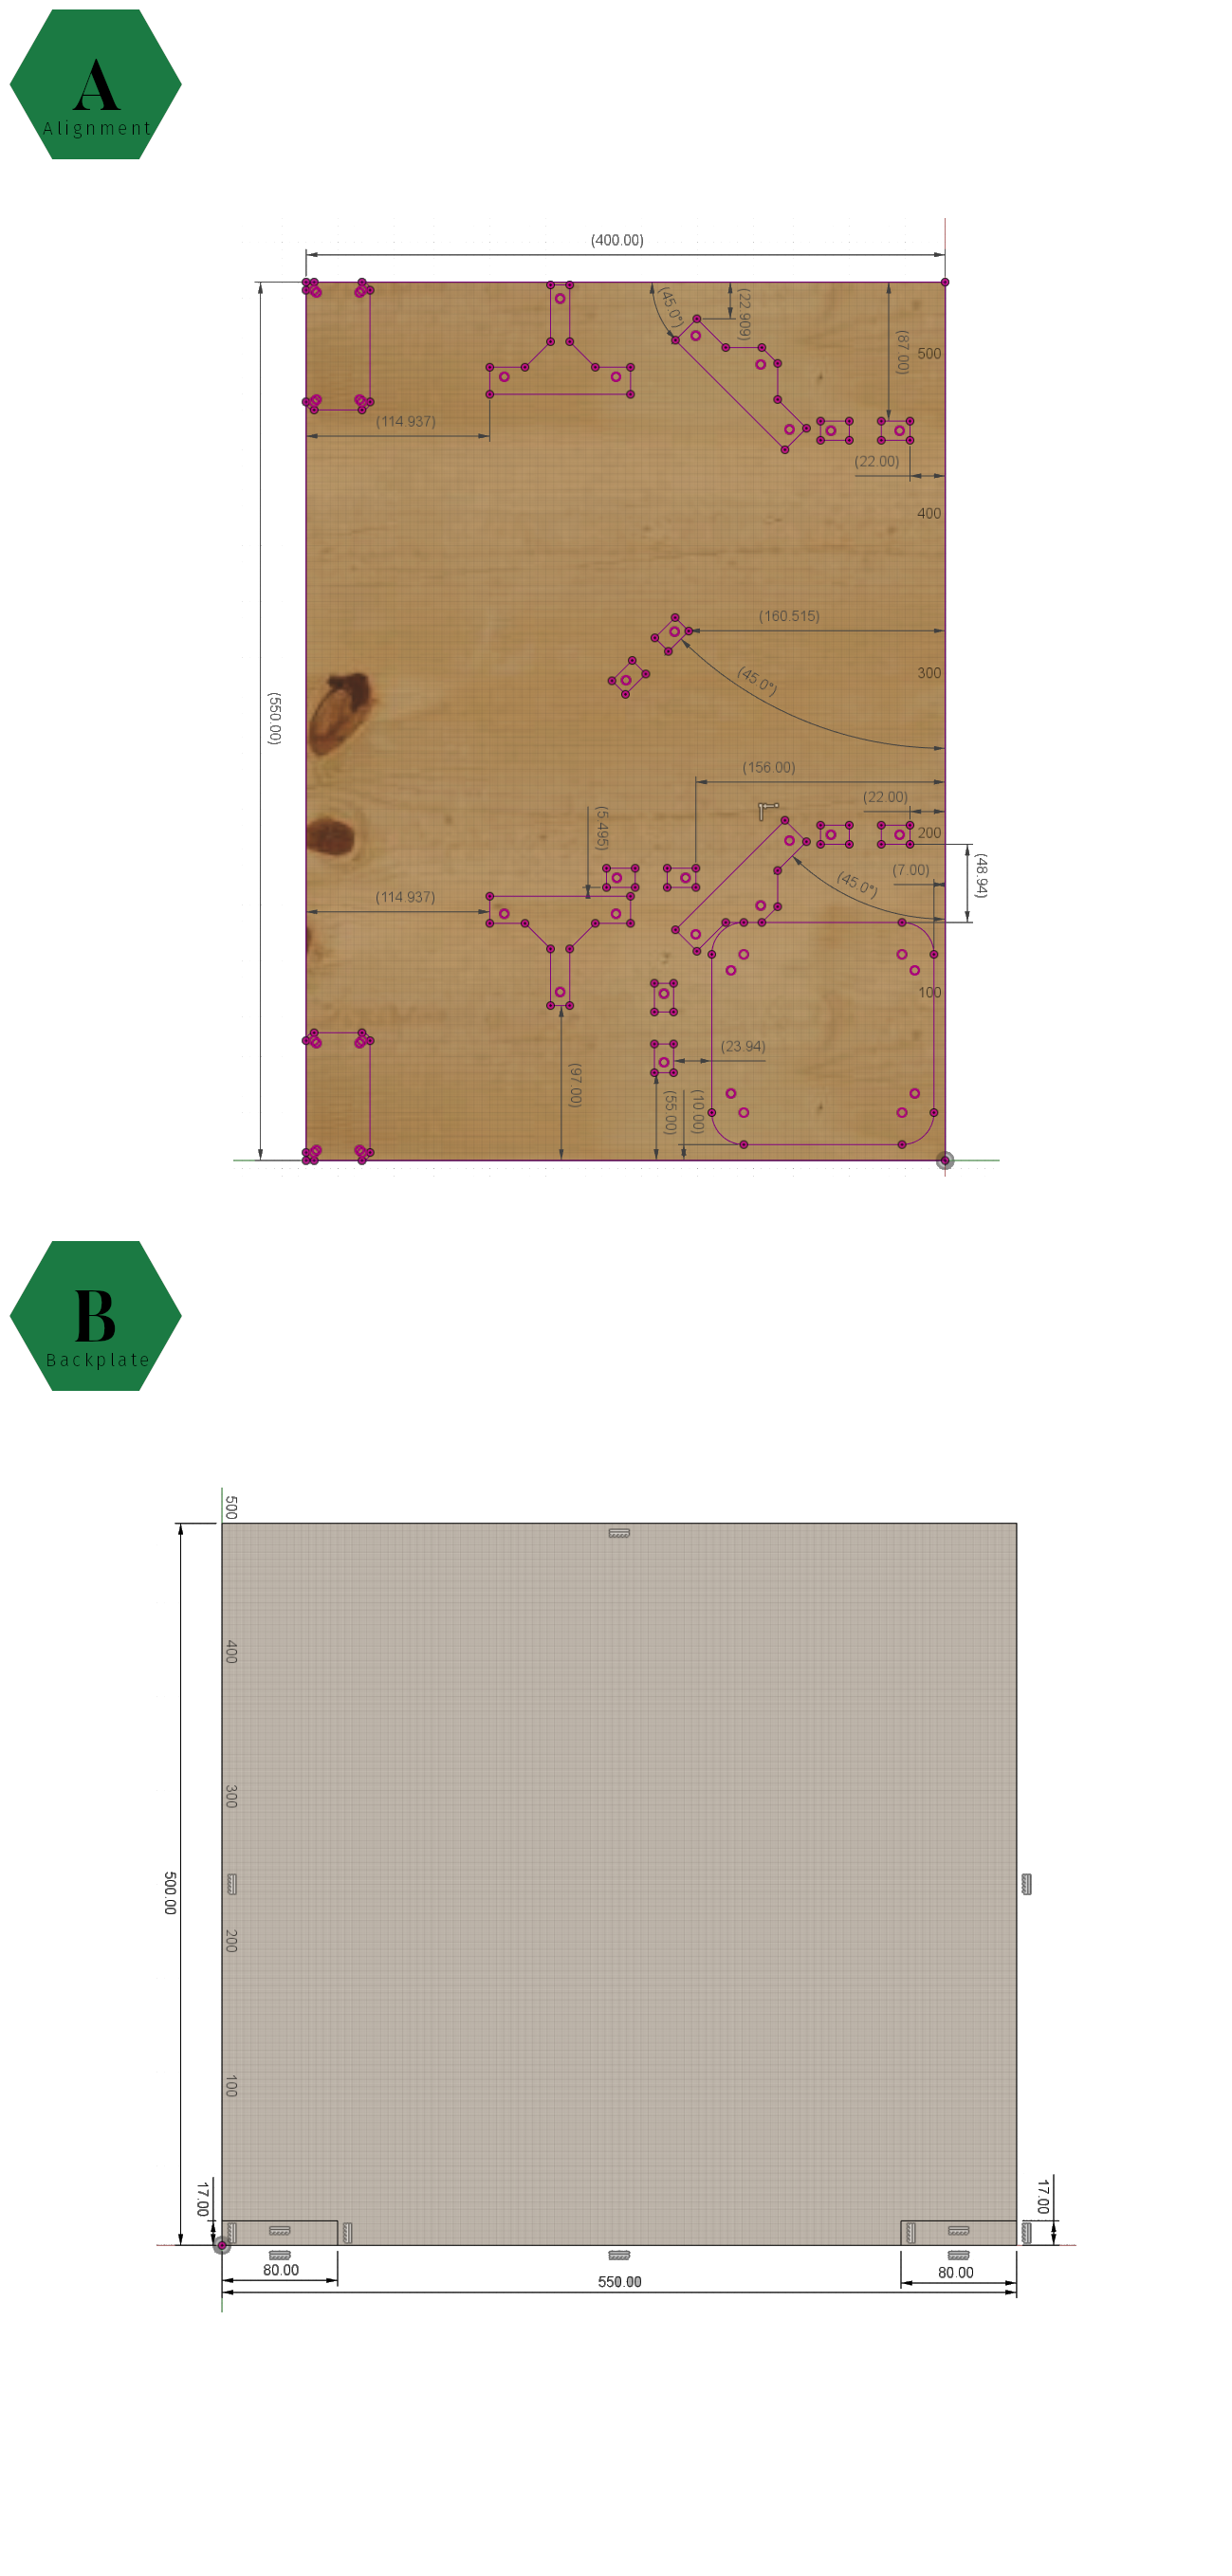
\includegraphics{images/Assembly18.png}%
{\captionof{figure}{Component Alignment on Base Plate \& Back Plate Size}}
\clearpage%